
\newpage
\chapter{Evaluation einer symmetrischen Antenne}

Das Abstrahlverhalten von Loop und Dipol Antennen ist im Fernfeld identisch. Im Fernfeld steht das E- und das H-Feld senkrecht aufeinander. Senkrecht zum E- und H-Feld zeigt sich der Ausbreitungsvektor. Die elektrischen und
magnetischen Feldkomponenten sind in Phase. Daher wird im Fernfeld Wirkleistung in transversale Raumrichtung
übertragen. Das elektrische und magnetische Feld hat nur Komponenten in der Ebene senkrecht zur Ausbreitungsrichtung.
Man spricht von einer ebenen Welle. Sie wird vom E- und H-Feldvektor aufgespannt  und bewegt sich in
Transversalerrichtung fort. Die Kugelwelle bewegt sich im Raum fort, bis die gesamte Energie absorbiert ist. Die Amplituden der E- und H-Vektoren
nehmen mit steigendem Abstand $r$ um den Faktor $1/r$  ab. Der Zusammenhang zwischen E- und H- Feld ist
durch die intrinsische Wellenimpedanz $\eta$ gegeben. Näheres zu den Feldvektoren und der Feldausbreitung ist im Kapitel \ref{sec:NahundFern} gezeigt. Der Wellenwiderstand im Vakuum zeigt(\ref{eq:WellenImpedanzZ0}) \cite{Harrington-TimeHarmonic},\cite{Emant}.
\begin{equation}\label{eq:WellenImpedanzZ0}
Z_{0}=\dfrac{E}{H}=\sqrt{\dfrac{\mu}{\epsilon}}=377\Omega
\end{equation}
Die Ausrichtung des E-Feldes ist bei den Loop- und  Dipolantennen um 90 Grad verschoben. 
Im Nahfeld sind die induktiven Anteile des elektromagnetischen Wechselfeldes bei den Loop Antennen dominant. Im Gegenzug ist das Nahfeld der Dipol Antenne  kapazitiv. Man nennt die Dipolantenne deshalb E-Feld Antenne.  Die Loop Antenne wird oft H-Feld Antenne genannt. Das Abstrahlverhalten dieser beiden Antennen ist in den Kapiteln \ref{sec:DipolAntenne} und \ref{sec:LoopAntenneTheorie} aufgezeigt. Die Abbildung \ref{fig:FerdVektorEinheistsvektor} zeigt einen Poynting-Vektor im  kugelkoordinaten und im kartesischen Koordinatensystem. Am Ende des Poynting-Vektors $\vec{r}$  befindet sich der Punkt P. Beim Punkt P sind die Einheitsvektoren mit den dazugehörenden  E- und H-Feldvektoren ersichtlich\cite{Emant}. Der Vektor ${E}_r$ zeigt die Richtung des Leistungstransports an.\\



%%%%%%%%%%%%%%%%%%%%%%%%%%%%%%%%%%%
\begin{figure}[!ht]
\begin{center}
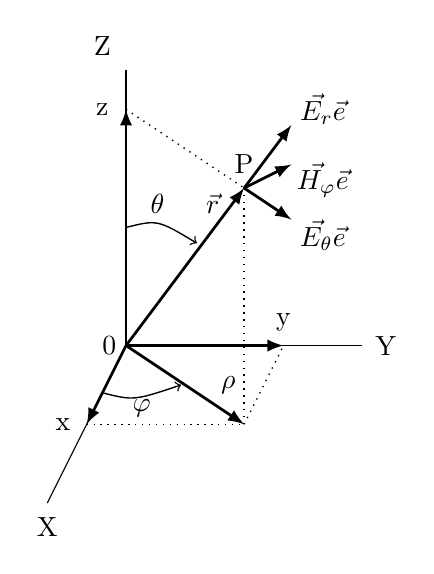
\begin{tikzpicture}
	\draw (4,4) -- (3,2)node at (3, 1.7) {X};%Fadenkreuz x
	\draw (4,4) node[left] {0} -- (7,4)node at (7.3, 4) {Y};%Fadenkreuz y
	\draw (4,4) -- (4,7.5)node at (3.7, 7.8) {Z};%Fadenkreuz z
	
	\draw[line width=1pt, ->, >=latex](4, 4)  -- (3.5, 3) node at (3.2, 3) {x};
	\draw[line width=1pt, ->, >=latex](4, 4)  -- (6, 4) node at (6, 4.3) {y};
	\draw[line width=1pt, ->, >=latex](4, 4)  -- (4, 7) node at (3.7, 7) {z};
	
	\draw[line width=0.5pt, style=dotted](3.5, 3) -- (5.5, 3);%Projektion y Rcihtung
	\draw[line width=0.5pt, style=dotted](5.5, 3) -- (6, 4);%Projektion x Rcihtung
	
	\draw[line width=1pt, ->, >=latex](4, 4)  -- (5.5, 3) node at (5.3, 3.5) {$\rho$};
	
	\draw[line width=1pt, ->, >=latex](4, 4)  -- (5.5, 6) node at (5.1, 5.8) {$\vec{r}$}  node  at (5.5, 6.3){P};
	
	\draw[line width=0.5pt, style=dotted](5.5, 3) -- (5.5, 6);%Projektion p zu \vec{r}
	\draw[line width=0.5pt, style=dotted](4, 7) -- (5.5, 6);%Projektion von z zur \vec{r}
	
	\coordinate (A) at (4, 5.5);
	\coordinate (B) at (4.9, 5.3);
	\coordinate (a) at (4.4, 5.6);
	\draw[line width=0.5pt, cap=round,->](A) .. controls (a) .. (B) node at (4.4, 5.8){$\theta$};
	
	\coordinate (C) at (3.7, 3.4);
	\coordinate (D) at (4.7, 3.5);
	\coordinate (c) at (4.1, 3.3);
	\draw[line width=0.5pt, cap=round,->](C) .. controls (c) .. (D) node at (4.2, 3.2){$\varphi$};
	
	%Einheitsvektoren
	\draw[line width=1pt, ->, >=latex](5.5, 6)  -- (6.1, 6.8) node at (6.5, 7) {$\vec{E_{r}}\vec{e}$};
	\draw[line width=1pt, ->, >=latex](5.5, 6)  -- (6.1, 5.6) node at (6.5, 5.4) {$\vec{E_{\theta}}\vec{e}$};
	\draw[line width=1pt, ->, >=latex](5.5, 6)  -- (6.1, 6.3) node at (6.5, 6.1) {$\vec{H_{\varphi}}  \vec{e}$};
	
\end{tikzpicture}
\end{center}
	\caption{Feldvektor mit Einheitsvektoren}
	\label{fig:FerdVektorEinheistsvektor}
\end{figure}
Die Oberfläche  der elektromagnetischen Welle nimmt mit steigendem Abstand $r$ von der Antenne  zu. Ebenfalls nimmt die Beugung der Kugelwelle immer mehr ab. Ist der Abstand $r$ genügend gross, so kann die Welle lokal als ebene Wellenfront angenommen werden. Bei Distanzen von mehr als $2\lambda$ kann das Fernfeld angenommen werden. Es gilt das Fernfeldkriterium. Bei einer Zielfrequenz von 2.45 Ghz, bei der die Bluetooth Antenne sendet, tritt das Fernfeld wie in (\ref{eq:Fernfeld}) gezeigt nach 24 cm auf.


\begin{eqnarray}
\lambda &=\dfrac{c}{f} \\
\lambda &=\dfrac{3*10^{8} [m/s]}{2.45*10^{9} [1/s]}=0.12m\\ 
2\lambda &= Fernfeldkriterium\\ 
2\lambda &= 2*0.12[m] =0.24 [m] \label{eq:Fernfeld}
\end{eqnarray}

Es ist wahrscheinlich, dass die meisten  Tuchfliegerpiloten ein Fluginstrument auf dem Schoss getragen. Dabei wird das Gerät in einer Hülle mit Bändern am Oberschenkel befestigt. Ein Mobiltelefon, welches sich am Arm des Piloten oder in einer Brusttasche befindet, ist  mehr als $2\lambda$ entfernt und somit im Fernfeld. Da sowohl die Loop- als auch die Dipolantenne ein Torus ähnliches Fernfeld aufzeigen und die Position der neuen Bluetooth Antenne für beide Antennen dieselbe sein wird, sind die Nahfeldeigenschaften der Antennen von Bedeutung.

\section{Eigenschaften einer Antenne für den Einsatz in der \\ \glqq Connect 1\grqq \  Serie}\label{sec:EigenschaftenAntenne}
Die 2.4 GHz Bluetooth Antenne wird im Gerät \glqq Connect 1\grqq \  der Flytec AG eingesetzt. Dies ist ein kompaktes Handgerät, welches den Piloten eines Tuchfliegers mit Informationen versorgt. Die Geräteabmessungen sind 142 x 88 x 23 mm (L x B x H). Der Raum, den die neue Antenne einnehmen wird, ist nicht derselbe wie in der Vorgängerversion. Für die neue Positionierung der Antenne ist der Hohlraum zwischen der Seitenwand des ABS Kunststoffgehäuses und der Hauptplatine  vorgesehen. Das mögliche Antennenvolumen beschränkt sich somit auf 55 x 3.5 x 10 mm (L x B x H).\\
Die Speisung der neuen Bluetooth Antenne soll nicht wie bis anhin asymmetrisch sein. Wie der Antennenfusspunkt mit der Quelle verbunden wird, ist zum jetzigen Zeitpunkt noch nicht definiert. Mögliche symmetrische Verbindungen sind:
\begin{itemize}
\item Microstrip   
\item Zweidrahtleitung
\item Zweidrahtleitung in Form eines Koaxialkabels
\end{itemize}
Die symmetrische Verbindung zwischen Quelle und Antenne hat den Vorteil, dass die bis anhin verwendeten Baluns für die Umwandlung des symmetrischen Ausgangs des Transceivers nicht mehr benötigt werden. Die passive Anpassung in Form der Baluns bringt bis anhin eine Dämpfung zwischen 6dB und 9dB mit sich. Die grosse Streuung kommt durch Bauteiltoleranzen zustande.\\
Diese Baluns waren bei der ersten Hardware Version des \glqq Connect 1\grqq \ Geräts notwendig, da für die Bluetooth Verbindung eine Monopolstabantennen verwendet wurde. Monopolstabantennen werden asymmetrisch gespeitst, daher musste der symmetrische Ausgang des Transceivers mit Hilfe von einem Balun angepasst werden. Der Balun wird aufgrund des zukünftigen, symmetrischen Antennendesign nicht mehr nötig sein. Die Ausgangsimpedanz $Z_{aus}$ des verwendeten Texas Instruments CC2541 Transceivers ist bei einer Frequenz von 2.440 GHz bei $(70+j30)$ Ohm. Dies entspricht einer komplexen Ausgangsimpedanz. \\
Bei den in dieser Arbeit gemachten Aussagen zu den Simulationen wurde jedoch eine reelle Quellimpedanz von $(50+j0)$ Ohm angenommen. In der ersten Betrachtung steht das Abstrahlverhalten und nicht die Anpassung an die Quelle im Fokus. Eine optimale Anpassung kann mit der im Kapitel \ref{sec:AnpassungReflexionen} beschiebenen Theorie gefunden werden.\\
Das Ersatzschaltbild in der Abbildung \ref{fig:ESBantenne} zeigt die wesentlichen Parameter einer Antenne, die für eine Beurteilung der Abstrahleffizienz notwendig sind. Es sind dies:
\begin{itemize}
\item $R_{v}$
\item $R_{rad}$
\item $Z_{ant}$
\end{itemize}
Weitere wichtige Eigenschaften, die für die Auswahl eines Antennentyps in ein kompaketes Handgerät zu berücksichtigen sind:
\begin{itemize}
\item Directivity D
\item Nahfeldtyp
\item Detuning durch das Umgebungsmaterial
\item Kopplung mit anderen im Gerät vorhandenen Antennen
\item Wirkungsgrad der Antenne
\end{itemize}


%%%%%%%%%%%%%%%%%%%%%%%%%%%%%%%%%%%%%%%%%%%%%%%%%%%
\begin{figure}[!ht]%ESB Antenne
	\begin{center}
	\begin{tikzpicture}
%	\draw[line width=1.5pt](7, 1.5) rectangle (12, 5.5) node at (9.5, 6) {Anpassungsnetzwerk};
%%%%%%%
%Zuleitung
	\draw[line width=1.5pt](8, 5)  -- (13.5, 5);
	\draw[line width=1.5pt](8, 2)  -- (16, 2);
%%%%%%%%
	\draw[line width=1.5pt, *-](12, 5)  -- (13.5, 5);
	\draw[line width=1.5pt, *-](12, 2)  -- (16, 2);
	\draw[line width=1.5pt](13.5, 4.75) rectangle (14.5, 5.25) node at (14, 5.5) {$R_{v}$};
	\draw[line width=1.5pt](14.5, 5)  -- (16, 5);
	\draw[line width=1.5pt](16, 5)  -- (16, 4.4);
	\draw[line width=1.5pt](15.75, 3.4) rectangle (16.25, 4.4) node at (17, 3.9) {$R_{rad}$};%Rrad
	\draw[line width=1.5pt](16, 3.4)  -- (16, 2.8);
	\draw[line width=1.5pt](15.75, 2.8)  -- (16.25, 2.8);%Kondensator oben
	\draw[line width=1.5pt](15.75, 2.6)  -- (16.25, 2.6);%Kondensator unten
	\node at (17, 2.7) {$X_{ant}$};
	\draw[line width=1.5pt](16, 2.6)  -- (16, 2);
	
	\draw[line width=1.5pt, ->, >=latex](8, 4)  -- (9.5, 4) node at (8, 3.5) {$P_{ein}$};
	\draw[line width=1.5pt, ->, >=latex](12, 4)  -- (13.5, 4) node at (13, 3.5) {$P_{ant}$};
	

%	\draw [-latex,line width=1.5pt](11.5,1) |-(13,2.5) node at (11.5, 0.5) {$Z_{ant}$};
	
	\node at (19.5, 6) {$\eta_{rad}=\dfrac{R_{rad}}{R_v+R_{rad}}$};
	\node at (11.5, 6) {$\eta_{tot}=\dfrac{P_{rad}}{P_{ein}}$};
	
	\node at (18, 2.7) {$\varepsilon$};
	\node at (18.5, 2.7) {$\delta$};
	
	\draw[->,line width=0.5pt,decorate, decoration=snake ](18, 4.1) -- (19.5, 4.6);
	\draw[->,line width=0.5pt, decorate, decoration=snake](18, 3.9) -- (19.5, 3.9);
	\draw[->,line width=0.5pt, decorate, decoration=snake](18, 3.7) -- (19.5, 3.1);
	\node at (20, 3.9) {$P_{rad}$};
	%%%%%%%%%%
	%Zanat
		\draw[line width=1.5pt, decorate, decoration=brace] (13, 1) -- (16.5, 1) node at (14.75, 0.5) {$Z_{ant} =  R_v + R_{rad} + X_{ant}$};
	%%%%%%%
	%%%%%%
	%REFLEXION
	\coordinate (A) at (9, 1);
	\coordinate (B) at (9, 0);
	\coordinate (a) at (12, 0.5);
	\draw[line width=1.5pt, cap=round,->](A) .. controls (a) .. (B) node at (8.5, 0.5) {$\Gamma$};
	%%%%%%%%%
	\end{tikzpicture}
	\end{center}
\caption{Ersatzschaltbild einer Antenne}
\label{fig:ESBantenne}
\end{figure}
%%%%%%%%%%%%%%%%%%%%%%%%%%%%%%%%%%%%%%%%%%%%%%%%%%%%%%%%%%%%

\newpage
Der $R_{v}$ vereint die elektrischen Verluste, die in den Leitern und an den Übergängen zu Stande kommen. Ebenfalls kann der $R_{rad}$ nicht einfach ausgemessen werden. $R_{rad}$ entspricht dem Widerstand der benötigt wird, um  die abgestrahlte Leistung in Wärme umzuwandeln. Die Abstrahlleistung ist vom Antennenstrom abhängig. Dieser wird stark von der frequenzabhängigen Anpassung beeinflusst.\\
Das Verhältnis von $R_{rad}$  zu $R_{v}$ wirkt direkt in die Abstrahleffizienz $\eta_{rad}$ ein. \\
Die Antennenreaktanz ist in der Abbildung \ref{fig:ESBantenne} als $X_{ant}$ in Form eines Kondensators abgebildet. Die dielektrischen Verluste des Winkels $\delta$ wirken ebenfalls in den $R_{v}$.\\
Die drei Komponenten $R_{v}$, $R_{rad}$ und $X_{ant}$ ergeben zusammen die gesamte Antennenimpedanz $Z_{ant}$. Dieser Zusammenhang ist  in den Abbildungen \ref{fig:ESBantenne} und \ref{fig:ESBantenneZant} zu erkennen. Wie aus Kapitel \ref{sec:Speisung} bekannt ist, stellt das Verhältnis der Leitungsimpedanz $Z_L$ zur Antennenimpedanz $Z_{ant}$ ein Mass für die in die Antenne übertragene Leitungsenergie dar. Ein weiteres wichtiges Antennenkriterium ist die Effizienz $\eta$ einer Antenne.  Man unterscheidet zwischen der Abstrahleffizienz und der totalen Effizeienz der Antenne. Die Abstrahleffizienz $\eta_{rad}$ wie gebildet aus:
\begin{equation}
\eta_{rad}=\dfrac{R_{rad}}{R_v + R_{rad}}=\dfrac{P_{rad}}{P_{ant}}
\label{eq:eta_rad}
\end{equation}
Die total Abstrahleffizenz $\eta_tot$ wird gebildet aus:
\begin{equation}
\eta_{tot}=\dfrac{P_{rad}}{P_{inc}}
\label{eq:eta_tot}
\end{equation}
Für die gilt:
\begin{enumerate}[leftmargin=2cm]
   \item[] $\eta_{rad}$: Abstrahleffizienz [$\%$] 
   \item[] $\eta_{tot}$: Die total Abstrahleffizienz [$\%$] 
   \item[] $R_{rad}$: Strahlungswiderstand einer Antenne [$\Omega$]  
   \item[] $R_v$: Antennenverluste [$\Omega$] 
   \item[] $P_{rad}$: Die von der Antenne abgestrhalte Leistung  [W] 
   \item[] $P_{ant}$: In die Antenne eindringende Leistung  [W 
   \item[] $P_{inc}$: Die von der Zuleitung zugeführte Leistung  [W] 
\end{enumerate} 

\section{Dipol Antenne}
Die Dipol Antenne ist eine häufig vorkommende Antennenform.  Dipol Antennen gibt es in einer grossen Zahl verschiedener Ausführungen. Ihre Abstrahlverhalten ändert sich mit ihren geometrischen Eigenschaften. Die Antennen werden oft ihn Kategorien entsprechend ihrer Länge eingeteilt. Eine Dipolarmlänge entspricht der halben Länge des Dipols und ist im folgenden Kapitel als $l$ bezeichnet. Dipol Antennen werden oft in die  vier typische Gruppen eigeteilt. 
\begin{itemize}
\item $2l<< \lambda/2 $
\item $2l = \lambda/2 $
\item $2l = \lambda $
\item $2l>> \lambda $
\end{itemize} 
Die Dipolantenne, bei der $2l=\lambda/2$ entspricht, wird oft Referenzdipol oder Halbwellendipol genannt. Wird der Halbwellendipol mit seiner Resonanzfrequenz $f_{res}$ angesteuert, tritt ein maximales Schwingen des Dipols auf. 

%%%%%%%%%%%%%%%%%%%%%%%%%%%%%%%%%%%%%%%%%%%%%%%%%%%
\begin{figure}[!ht]%ESB Antenne
	\begin{center}
	\begin{tikzpicture}
	\draw[line width=1.5pt](5, 2) circle (0.5) node at (5, 2) {AC};
	\draw[line width=1pt, -*](4.8, 2.45) -- (4.8, 3.6);%nach oben links
	\draw[line width=1pt, -*](5.2, 2.45) -- (5.2, 3.6);%nach oben rechts
	
	\draw[line width=3pt](4.8, 3.5) -- (2, 3.5)node at (3.4, 3) {$l$};%links
	\draw[line width=3pt](5.2, 3.5) -- (8, 3.5)node at (6.6, 3) {$l$};%rechts
	
	\draw[line width=1pt, ->, >=latex](3.8, 3.7)  -- (3, 3.7) node at (3.4, 3.9) {I};%Strompfeil links
	\draw[line width=1pt, ->, >=latex](6.2, 3.7)  -- (7, 3.7) node at (6.6, 3.9) {I};%Strompfeil rechts	
	
	\coordinate (A) at (2, 3.5);%Bogen
	\coordinate (B) at (8, 3.5);
	\coordinate (a) at (5, 5.2);
	\draw[line width=1pt, cap=round](A) .. controls (a) .. (B);
	
	\draw[line width=0.5pt, style=densely dashed](1.8, 3.5) -- (1.8, 5.5);%nach oben links
	\draw[line width=0.5pt, style=densely dashed](8.2, 3.5) -- (8.2, 5.5);%nach oben rechts
	\draw[line width=0.5pt, style=densely dashed](1.7, 5.4) -- (8.3, 5.4) node at (5, 5.7) {$\lambda/2$};%langer Strich
	
	\end{tikzpicture}
	\end{center}
\caption{Horizontalpolarisierter Halbwellendipol}
\label{fig:HalbWellenDipolHorizontal}
\end{figure}
%%%%%%%%%%%%%%%%%%%%%%%%%%%%%%%%%%%%%%%%%%%%%%%%%%%%%%%%%%%%

\newpage
Gegenüber idealen Betrachtungen muss die Länge des $\lambda /2$ Dipols um den Verkürzungsfaktor kürzer gewählt werden, um  die gewünschte Frequenz zu erhalten. Die Verkürzung  ist in der Abbildung \ref{fig:HalbWellenDipolHorizontal} gezeigt und abhängig von der Geometrie, dem Material der Antenne und dem umgebenden Materialien \cite{Hcuno}.
Der Verkürzungsfaktor ist für das Antennendesign entscheidend. Daher soll an dieser Stelle etwas genauer auf die Ausbreitungsgeschwindigkeit einer Welle im Medium eingegangen werden.
Die Ausbreitungsgeschwindigkeit, die Wellenlänge und die Frequenz sind voneinander abhängige Grössen. 
Die Ausbreitungsgeschwindigkeit beschreibt, wie schnell sich ein Signal im Medium, das heisst im Vakuum, in der Luft oder in einer Leitung , fortpflanzt. Die Ausbreitungsgeschwindigkeit wird mit dem Buchstaben $c$ abgekürzt. Eine elektromagnetische Welle breitet sich im
Vakuum mit $c_0 = $ 299'792’458 [m/s] aus. In der Praxis kann mit 300000 km/s gerechnet werden.
Die Wellenlänge beschreibt die Länge einer vollständigen Schwingung. Sie ist der kleinste Abstand zweier phasengleicher Punkte einer Welle. Die Wellenlänge wird mit dem Buchstaben $\lambda$  abgekürzt. Die Frequenz beschreibt  die Anzahl der Schwingungen in einem  Zeitraum von einer Sekunde. Die Einheit der Frequenz ist Herz und wird mit Hz abgekürzt. Ein Herz beschreibt eine Schwingung pro Sekunde [1/s] \cite{Verkuertzungsfaktor}.
Es gilt folgender Zusammenhang:\\
Die Ausbreitungsgeschwindigkeit ist in einem homogenen Medium konstant. Wird die Frequenz erhöht, muss  die Wellenlänge kürzer werden $\lambda = \dfrac{c}{f}$. Geht man von einer konstanten Frequenz, aber von sich ändernden Medien aus, so gilt: \\
Die Geschwindigkeit mit der sich eine elektromagnetische Welle im Medium fortbewegt, muss um einen Faktor $V$ kleiner  als die Lichtgeschwindigkeit $c_0$ sein.\\
Die Fortpflanzungsgeschwindigkeit $v_p$ gibt die Geschwindigkeit einer Welle im Medium an  $v_p=c_0*V $. Der Faktor $V$ gibt den Verkürzungsfaktor an, um den $v_p$ kleiner als die Lichtgeschwindigkeit $c_0$ ist. \\
Der Verkürzungsfaktor V ist also definiert durch:
\begin{equation}
V=\dfrac{v_p}{c_0}=\dfrac{c_0}{\sqrt{\epsilon_0 \mu_0}}
\end{equation}
Wobei $\varepsilon_0$ die effektive Permittivitätszahl
 und $\mu_0$ die Permeabilitätszahl des Mediums ist. Beide Grössen sind  frequenzabhängig. Für die Berechnung des Verkürzungsfaktors in Leitungen werden kurze Rechteckpulse betrachtet, die hohe Frequenzen beinhalten, bei denen sich $\varepsilon$ einem Grenzwert nähert. Für Leitungen aus Kupfer und Aluminium gilt weiterhin, dass $\mu_r \approx 1$ entspricht. Bei einer verlustfreien Leitung gilt \cite{Verkuertzungsfaktor_wiki}:
\begin{equation}\label{V_verlustfreie_Leitung}
V=\dfrac{1}{c_0 \sqrt{L'C'}} 
\end{equation}
Für (\ref{V_verlustfreie_Leitung}) gibt $C'$  den Kapazitätsbelag und $L'$ den Induktivitätsbelag  der Leitung an und $c_0$ entspricht der Vakuumlichtgeschwindigkeit einer Welle.
\begin{equation}\label{eq:v}
\lambda=\dfrac{v_p}{f}
\end{equation}  
Aus (\ref{eq:v})  ist ersichtlich, dass die Wellenlänge $\lambda$ bei gleichbleibender Frequenz $f$ und sinkender Geschwindigkeit $v_p$ kürzer wird. 
Um den Verkürzungsfaktor einer Antenne zu berechnen, müssen alle elektrischen, magnetischen und Geometrischen Parameter der Antenne und der unmittelbaren Umgebung bekannt sein. Falls diese Parameter  nicht bekannt sind, muss mit empirischen Versuchsreihen die Ausbreitungsgeschwindigkeit ermittelt werden.\\

\newpage
Die Simulationen zeigen den Verkürzungseffekt, in dem die resultierende Antennenfrequenz tiefer als erwartet ist. Das heisst, aus $\lambda = \dfrac{c}{f}$ kann die Formel nach $f$ umgestellt werden. Das ergibt $f=\dfrac{c}{\lambda}$. Setzt man für $\lambda$ die Länge der Antennenstruktur in Meter ein, so resultiert eine Frequenz $f$. Da die Ausbreitungsgeschwindigkeit in einem verlustbehafteten Leiter entspricht nicht der Vakuumausbreitungsgeschwindigkeit einer elektromagnetischen Welle $c_0$, sondern $v_p=V c_0$. Daher  wird die Resonanzfrequenz tiefer sein als erwartet. Erst nach einer Kürzung der Antennenstruktur um den Faktor $v_p$ wird die Resonanzfrequenz auf die gewünschte Siganlfequenz steigen. Um die gewünschte Zielfrequenz zu erhalten, muss die effektive Ausbreitungsgeschwindigkeit $v_p$ einer Antennenstruktur bekannt sein.\\

%Weiter Komentar wiso es sich eine Verkürzung einstellt
%H. Cuno, Vorbereitung auf die Amateurfunklizenzprüfung, Frech-VerlagStuttgart, 1976 
Ideale Betrachtung geht von einem unendlich dünnen Leiter aus, wobei der Dipol im ungestörten Raum betrieben wird. Aufgrund der geforderten mechanischen Festigkeit müssen reale Dipole eine gewisse Mindestdicke aufweisen. Die Umgebung des Dipols kann ebenfalls nicht als völlig als freier Raum angenommen werden. Es befindet sich immer eine Quelle oder eine Zuleitung in der Nähe von realen Antennen. \\

Wenn sich eine $\lambda /2$ lange Antenne vertikal über der Erde befindet,  ergibt sich für ein Strahlungsdiagramm mit den folgenden Eigenschaften: 
Die Horizontalcharakteristik des vertikalen Halbwellendipols ist kreisförmig. Das Strahlungsdiagramm ist unabhängig vom Azimutwinkel $\varphi$ in der Horizontalebene des Dipols. Die Vertikalcharakteristik des  Halbwellendipols erscheint jedoch gerichtet. Dies bedeutet, es besteht eine Abhängigkeit vom Winkel $\theta$ \cite{zinke1965lehrbuch}. 
%O. Zinke, H. Brunswig, Lehrbuch der Hochfrequenztechnik, Band 1, 4. Auflage,Springer-Verlag, Berlin Heidelberg New York, 1990
Nach \cite{elliott1981antenna} lassen sich die folgenden Aussagen für die Gewichtungsfunktion  eines Dipols der vertikal über der Erde polarisiert ist treffen\cite{elliott1981antenna}:

\begin{equation}\label{eq:FDipolTheat}
F(\theta,\frac{l}{\lambda}=\dfrac{1}{2})=-\dfrac{2I_{m}}{k}\dfrac{\cos\left(\dfrac{\pi}{2}\cos\theta\right)}{\sin\theta}
\end{equation}

%Braucht es eventuell noch ein Bild

Die Nahfeldeigenschaften der Dipol Antenne weisen ein starkes E-Feld auf. Dieses zeigt eine Richtungsabhängigkeit des Winkels $\theta$. Die starken E-Felder polarisieren alle Dielektrika in unmittelbarer Nähe des Dipols. Dies führt zu dielektrischen Verlusten. Diese steigen mit der Frequenz des Wechselfeldes. Die dielektrischen Verluste können als Widerstände in Serie zu den idealen Komponenten eines Ersatzschaltbildes gedacht werden. Sie stellen die äquivalente Verlustleistung an einer Komponente dar. Die Verlustenergie wird für das Polarisieren des umgebenden Dielektrikums benötigt. Die Ausrichtungsenergie ist Verlustenergie und kann somit nicht abgestrahlt werden.
Das Dielektrikum ist ein elektrisch nicht leitendes Material das vom elektrischen Feld durchdringt wird. Die Feldgrössen des Dielektrikums sind die elektrische Feldstärke E und die elektrische Flussdichte D. Im elektrostatischen Fall, das heisst im zeitlich konstanten Fall und in einem isotropen Medium, ist die Flussdichte D durch die Primitivität $\varepsilon $ und durch die elektrische Feldstärke E beschrieben. Die folgende Beziehung in (\ref{eq:FlussdichteD}) zeigt die Verknüpfung von $\varepsilon$  und des E-Feldes \cite{Emant}:
\begin{equation}\label{eq:FlussdichteD}
D=\varepsilon E
\end{equation}
Die Permittivität $\varepsilon$ setzt sich, wie in (\ref{eq:Epsilon}) ersichtlich, aus der elektrischen Feldkonstante $\varepsilon_0$ und der materialspezifischen, relativen Permittivität $\varepsilon_r$ zusammen:
\begin{equation}\label{eq:Epsilon}
\varepsilon = \varepsilon_r \varepsilon_0
\end{equation}
Die Permittivitäts Konstante $\varepsilon_{0}$ ist eine Naturkonstante. Sie erhält ihren Wert aus dem in (\ref{eq:Epsilon0}) ersichtlichen Zusammenhang. Die Konstante $\mu_{0}$ ist wie die Lichtgeschwindigkeit $c_0$ eine Naturkonstante und beschreibt die magnetische Feldkonstante. Sie ist definiert als \cite {WikiPermitt}: 
\begin{equation}\label{mu_0}
\mu_{0}=4\pi10^-7 [N/A^{2}] 
\end{equation}
\begin{equation}\label{eq:Epsilon0}
\varepsilon_{0} = \dfrac{1}{\mu_{0}c^{2}}=8.854187...[As/Vm]
\end{equation}
Da in einem Dielektrikum die Ladungsträger nicht frei beweglich sind, werden sie durch ein äusseres elektrisches Feld polarisiert. Dabei wird zwischen zwei Arten der Polarisation unterschieden:
\begin{itemize}
\item Verschiebungspolarisation
\item Orientierungspolarisation
\end{itemize}
Bei der Verschiebungspolarisation werden elektrische Dipole  induziert. Das heisst,  die Dipole entstehen durch geringe Ladungsverschiebung in den Atomen, Molekülen oder zwischen verschieden geladenen Ionen. In einem Wechselfeld schwingen die negativen Elektronenhüllen und die positiven Atomkerne gegenläufig hin und her.  Bei diesen Schwingungen entsteht  Wärmeenergie.  Diese kann gegenüber der Energie, die bei der Orientierungspolarisation entsteht,  vernachlässigt werden.  Die Bewegung des Atomkerns kann auf Grund seiner deutlich grösseren Masse  gegenüber der Elektronenhüllenbewegung vernachlässigt werden. Somit wird der Atomkern als ortsfest betrachtet. \\
Unter der Orientierungspolarisation versteht man die Ausrichtung ungeordneter, permanenter Dipole eines Isolators im elektrischen Feld. Bei einem Wechselfeld müssen sich die Moleküle ständig umorientieren, wodurch Wärmeenergie entsteht\cite{DielektrikumPolarisation}.\\
Im Nahfeld einer Antenne pendelt die nicht abgestrahlte Energie im Raum um die Antenne hin und her. Das Nahfeld baut sich auf und ab. Es wechselt  mit der Resonanzfrequenz $f_{r}$ seine Richtung. Die Moleküle im dielektrischen Raum um die Antenne werden bei jeder Schwingung neu polarisiert. Das bedeutet, die Moleküle werden zwei Mal pro Schwingung neu ausgerichtet.\\
Die im Dielektrikum gespeicherte Energie ist stark von der materialspezifischen, relativen Permittivität $\varepsilon_r $ abhängig.\\
Die dielektrischen Verluste führen bei Antennen  zu einem Detuning. Das Detuning ist kaum zu berechnen, jedoch kann es mit Hilfe von  Simulationen bestimmt werden. Das Detuning entsteht durch Verluste in und um die  Antenne.\\ 
Das Detuning kann auch eine Chance darstellen. Es ist denkbar, dass durch das Detuning und eine veränderte Antennenimpedanz eine Anpassung  entsteht die  eine wesentlich höhere Abstrahleffizienz $\eta_{overall}$ \ mit sich bringt. Weiter kann das Detuning eine Absenkung der Resonanzfrequenz hervorrufen, die sonnst nur mit einer Vergrösserung der Antennenstruktur möglich wäre. Das kann ein Vorteil sein, wenn die Platzverhältnisse sehr eingeschränkt sind.\\
Im Zusammenhang der Antennen und der reaktiven Nahfeldverlusten wird oft der Verlustwinkel genannt. Der Verlustwinkel beschreibt den Anteil der Wirkleistung zu Blindleistung elektrisch reaktiver Bauteile wie Spulen oder Kondensatoren bei einem sinusförmigem Spannungs- und Stromverlauf.\\
Der Verlustwinkel ist als $\arctan$ des Verhältnisses von Wirkleistung zu Blindleistung definiert. Dies ist  aus der Gleichung  \ref{eq:Verlustwinkel} ersichtlich. 
Je kleiner der Verlustwinkel ist, desto näher kommen die realen Bauteile ihrem idealen Verhalten. Eine ideale Induktivität hat einen Verlustwinkel von $0^\circ$. Ein idealer Kondensator hat ebenfalls einen Verlustwinkel von 0$^\circ$. Ein Verlustwinkel der grösser ist als $0^\circ$ führt zu Verlustwiderständen die in Serie zu den idealen Induktivitäten und Kapazitäten gerecht werden.\\
In der technisch realisierbaren Elektronik gibt es jedoch keine idealen Bauteile. Die Verluste in dem Bauteilen sind zudem stark frequenzabhängig.\\
Der Verlustwinkel  $\delta$  lässt sich über die komplexe Impedanz $Z$ oder über die Phasenverschiebung  $\varphi$  zwischen Strom $I$ und Spannung $U$ des Bauteils berechnen: 
\begin{align}
\label{eq:Verlustwinkel}
\delta &= \arctan \dfrac{ReZ}{ImZ}
\end{align}
\begin{align}
\label{eq:Verlustwinkel_aus_Phi}
\delta &= 90^\circ - |\varphi|
\end{align}
Die realen Ersatzschaltbilder von Spulen und Kondensatoren berücksichtigen die Verluste mit einem Widerstand $R$.
Die beiden Gleichungen (\ref{eq:VerlustwinkelSpule}) und (\ref{eq:VerlustwinkelKondensator}) zeigen die Verlustfaktoren an einer Spule $L$ und an einem Kondensator $C$:
\begin{equation}\label{eq:VerlustwinkelSpule}
\tan \delta = \dfrac{R}{\omega L}
\end{equation}
\begin{equation} \label{eq:VerlustwinkelKondensator}
\tan \delta = R \omega C
\end{equation}
In diesem Zusammenhang soll  die komplexe Permittivität $\varepsilon$ genannt werden:
\begin{equation} \label{eq:komplexePermitivität}
\varepsilon=\varepsilon_0(\varepsilon^{'}-j\varepsilon^{''})=\varepsilon_0\varepsilon^{'}\big(1-j\dfrac{\varepsilon^{''}}{\varepsilon^{'}}\big)
\end{equation}
In der Gleichung (\ref{eq:komplexePermitivität}) kommt das Verhältnis $\dfrac{\varepsilon^{''}}{\varepsilon^{'}}$ vor. Es ist klein für gute Dielektrika, welche über einen weiten Frequenzbereich annähernd konstant sind. Das Verhältnis von der Wechselstrom Permittivität $\varepsilon^{'}$ und des dielektrischen Verlustfaktors $\varepsilon^{''}$ ergibt den Verlustwinkel $\tan\delta$ \cite{elliott1981antenna}. 
\begin{equation} \label{eq:VerlustwinkelEpsilonPermitivität}
\dfrac{\varepsilon^{''}}{\varepsilon^{'}}=\tan\delta
\end{equation}


\subsection{Verwendung einer Dipolantenne}
Eine symmetrisch gespeisste Halbwellenantenne  ist eine einfach zu produzierende Antenne. Zwei elektrisch leitende Strahler mit je einer Länge von $\lambda/4$ und eine symmetrische Zuleitung stellen einen geringen Produktionsaufwand dar. Die halbe Wellenlänge als strahlende Leiterlänge bedeutet bei einer Siganlfrequenz von 2.45 GHz etwas weniger als $\lambda/2=0.006m$ Strahlerlänge. Ein Dipol mit der Länge von 6 cm ist im Schlitz zwischen der Hauptplatine und dem Gehäuse unterzubringen. 
Bei dieser Positionierung der  Antenne ist sie von sehr viel ABS Kunststoffmaterial umgeben, da das ganze Gehäuse aus ABS Kunsstoff besteht. Dieses Material ist elektrisch nicht leitend und nicht magnetisch. Alle Dipolantennen sind in ihrem unmittelbaren Umfeld starke E-Feld Strahler. Die Materialeigenschaften von ABS Kunststoff führen mit einem  $\varepsilon_r$ von ca. 4.2[As/Vm] bei 2.4 GHz zu einer erheblichen Energiespeicherung im reaktiven Nahfeld der Antenne. Daraus folgt eine  Abweichung der Ausbreitungsgeschwindigkeit, diese wiederum bringt ein Detuning der Antenne mit sich \cite{WikiPermitt}.\\

Das Abstrahlverhalten einer Dipolantenne ist $\theta$ abhängig. Der Richtfaktor,  auf englisch \textit{directivity} D genannt, ist bei Dipolantennen wie in  (\ref{eq:Directivity}) gezeigt   1.64 dBi.  Der Richtfaktor vergleicht die Leistungsdichte in der stärksten Abstrahlrichtung mit der Leistungsdichte eines isotropen Kugelstrahlers  bei gleicher abgestrahlter Leistung. Da die Dipolantenne in der Längsausrichtung an der Seitenkante des Geräts untergebracht wird, ergibt sich eine theoretische Nullstelle des elektromagnetischen Feldes in der Verlängerung der Antennenstruktur. Die  Abbildunge \ref{fig:DipolEFerd} zeigt die Nullstellen entlang der Ausrichtung des Dipols. Sie zeigt einen Schnitt durch das elektromagnetische Feld in der xz-Ebene. Das dargestellten Feld ist um die z-Achse rotationssymmetrisch. Die Absorbtion des elektromagnetischen Felds, wlche durch das Gerät ensteht, ist in der Abbildungen \ref{fig:DipolEFerd} nicht dargestellt.

%%%%%%%%%%%%%%%%%%%%%%%%%%%%%%%%%%%%%%%%%%%%%%%%%%%%
%\begin{figure}[!ht]%ESB Antenne
%	\begin{center}
%	\begin{tikzpicture}[scale = 0.8]
%	\draw[line width=1pt](5, 5) rectangle (8, 10) node at (6.5, 9.5) {Connect 1};
%	\draw[line width=1pt](5.3, 6.2) rectangle (7.7, 9);
%	\draw[line width=1pt, ->, >=latex](1, 1) -- (3, ) node at (3.2, 1) {x};
%	\draw[line width=1pt, ->, >=latex](1, 1) -- (1, 3) node at (1.2, 3) {y};
%	\draw[line width=1pt](1, 1) circle (0.2) ;\fill[fill=black](1, 1) circle (2pt);
%	\draw[line width=2pt] (5.15,5.3)--(5.15,6.8);%Antenne unten
%	\draw[line width=2pt] (5.15,7)--(5.15,8.5);%Antenne oben
%	\draw[line width=3pt](3.3, 6.9) ellipse (1.5 and 5);%Feld links
%	\draw[line width=3pt](6.9, 6.9) ellipse (1.5 and 5);%Feld rechts
%
%	\end{tikzpicture}
%	\end{center}
%\caption{Nullstelle des elektromagnetischen Feldes in der xy Ebene bei z = 0 in der Verlängerung der Antenne}
%\label{fig:xyFeld}
%\end{figure}
%%%%%%%%%%%%%%%%%%%%%%%%%%%%%%%%%%%%%%%%%%%%%%%%%%%%%%%%%%%%%
%\newpage
%Die Abbildung \ref{fig:xyFeld} zeigt schematisch die Feldausbreitung einer Dipolantenne, die sich in einer Lücke des  Geräts befindet. Es kommt zu einer Nullstelle in der Längsausrichtung der Antenne. Die Abbildung \ref{fig:xyFeld} zeigt das elektromagnetische Feld bei $\theta=90^\circ$. Es zeigt einen ebenen Schnitt auf der Höhe x=0. \\
%Die selbe Situation, aber aus einer anderen Perspektive auf das \glqq Connect 1\grqq \ Gerät zeigt die Abbildung  \ref{fig:xzFeld}. Die elektromagnetischen Feldlinien bilden Kreise radial um die Dipolstäbe. Die Abbildung  \ref{fig:xzFeld} zeigt das Feld bei y=0. Diese Felddarstellung beschreibt das Feld in der xy Ebene.
% %%%%%%%%%%%%%%%%%%%%%%%%%%%%%%%%%%%%%%%%%%%%%%%%%%%
%\begin{figure}[!ht]%ESB Antenne
%	\begin{center}
%	\begin{tikzpicture}[scale = 0.8]
%	\draw[line width=1pt](5, 5) rectangle (8, 6); %node at (9, 6) {Connect 1};
%	\draw[line width=1pt, ->, >=latex](3, 3) -- (5,3 ) node at (5.2, 3) {x};
%	\draw[line width=1pt, ->, >=latex](3, 3) -- (3, 5) node at (3.2, 5) {z};
%	\draw[line width=1pt](3, 3) circle (0.2) ;\fill[fill=black](3, 3) circle (2pt);
%	\draw [line width=2pt] (5.15,5.3)--(5.15,5.5);%Antenne
%	\draw[line width=3pt](5.1, 5.4) circle (1.5);%Feld
%	\end{tikzpicture}
%	\end{center}
%\caption{Elektromagnetisches Feld in der xz Ebene bei y = 0 }
%\label{fig:xzFeld}
%\end{figure}
%%%%%%%%%%%%%%%%%%%%%%%%%%%%%%%%%%%%%%%%%%%%%%%%%%%%%%%%%%%%
Der Strahlungswiderstand des $\lambda/2$ Dipols entspricht, wie aus  (\ref{RradDipol}) zu entnehmen ist, 73 Ohm. Dies ist ein theoretischer Wert und  kommt  nur im Freiraum zustande. Technisch realisierbare Halbwellendipole haben einen Strahlungswiderstand $R_{rad}$ kleiner als 70 Ohm. Zudem kommt  ein von der  Geometrie der Antenne abhängige Reaktanz $X_{ant}$ hinzu.\\
Die Reaktanz $X_{ant}$,  der Strahlungswiderstand $R_{rad}$ sowie der Verlustwiderstand $R_v$ ergeben die Antennenimpedanz. Diese wird $Z_{ant}$  genannt. Dieser Zusammenhang ist  in der Abbildung \ref{fig:ESBantenne} gezeigt. Sie zeigt eine Reaktanz  $X_{ant}$ die einen negativen Imaginärteil auf. Deshalb ist $X_{ant}$ in Form eines Kondensators gezeichnet.

%%%%%%%%%%%%%%%%%%%%%%%%%%%%%%%%%%%%%%%%%%%%%%%%%%%%
%\begin{figure}[!ht]%ESB Antenne mit Zant
%	\begin{center}
%	\begin{tikzpicture}
%%	\draw[line width=1.5pt](7, 1.5) rectangle (12, 5.5) node at (9.5, 6) {Anpassungsnetzwerk};
%	\draw[line width=1.5pt, *-](12, 5)  -- (13.5, 5);
%	\draw[line width=1.5pt, *-](12, 2)  -- (16, 2);
%	\draw[line width=1.5pt](13.5, 4.75) rectangle (14.5, 5.25) node at (14, 5.5) {$R_{v}$};
%	\draw[line width=1.5pt](14.5, 5)  -- (16, 5);
%	\draw[line width=1.5pt](16, 5)  -- (16, 4.4);
%	\draw[line width=1.5pt](15.75, 3.4) rectangle (16.25, 4.4) node at (17, 3.9) {$R_{rad}$};%Rrad
%	\draw[line width=1.5pt](16, 3.4)  -- (16, 2.8);
%	\draw[line width=1.5pt](15.75, 2.8)  -- (16.25, 2.8);%Kondensator oben
%	\draw[line width=1.5pt](15.75, 2.6)  -- (16.25, 2.6);%Kondensator unten
%	\node at (17, 2.7) {$X_{ant}$};
%	\draw[line width=1.5pt](16, 2.6)  -- (16, 2);
%	
%%	\draw[line width=1.5pt, ->, >=latex](6.5, 4)  -- (8, 4) node at (8, 3.5) {$P_{ein}$};
%%	\draw[line width=1.5pt, ->, >=latex](11.5, 4)  -- (13, 4) node at (13, 3.5) {$P_{ant}$};
%	
%
%%	\draw [-latex,line width=1.5pt](11.5,1) |-(13,2.5) node at (11.5, 0.5) {$Z_{ant}$};
%	
%%	\node at (17.5, 6) {$\eta_{rad}=\dfrac{R_{rad}}{Rv+R_{rad}}$};
%%	\node at (9.5, 7) {$\eta_{overall}=\dfrac{P_{rad}}{P_{ein}}$};
%	
%%	\node at (18, 2.7) {$\varepsilon$};
%%	\node at (18.5, 2.7) {$\delta$};
%%	
%%	\draw[->,line width=0.5pt,decorate, decoration=snake ](18, 4.1) -- (19.5, 4.6);
%%	\draw[->,line width=0.5pt, decorate, decoration=snake](18, 3.9) -- (19.5, 3.9);
%%	\draw[->,line width=0.5pt, decorate, decoration=snake](18, 3.7) -- (19.5, 3.1);
%%	\node at (20, 3.9) {$P_{rad}$};
%	
%	\draw[line width=1.5pt, decorate, decoration=brace] (13, 1) -- (16.5, 1) node at (14.75, 0.5) {$Z_{ant} =  R_v + R_{rad} + X_{ant}$};
%	\end{tikzpicture}
%	\end{center}
%\caption{Ersatzschaltbild einer Antenne mit $Z_{ant}$}
%\label{fig:ESBantenneZant}
%\end{figure}
%%%%%%%%%%%%%%%%%%%%%%%%%%%%%%%%%%%%%%%%%%%%%%%%%%%%%%%%%%%%%



%Der Strahlungswiderstand $R_{rad}$ des Halbwellen Dipols wird in der Gleichung \ref{eq:Rrrad} im Kapitel \ref{sec:kurzerDipol} berechnet. Man erhält für einen Dipol mit $2L = \frac{\lambda}{2}$ einen $R_{rad}$ von $15.7 \Omega $.

\newpage
\subsection{Simulationen eines Halbwellen Dipols}\label{sim_lamda2_Dipol}

Das Volumen, in dem eine Bluetooth Antenne untergebracht werden kann, ist in Kapitel \ref{sec:EigenschaftenAntenne} beschrieben. Das zur Verfügung stehende Volumen von 55 x 3.5 x 10 mm (L x B x H) wurde bei den Simulationen berücksichtigt. \\
Für die Simulationen wurden grosse Vereinfachungen getroffen.\\
Der ABS Kunststoff ist mit einem $\varepsilon_r $ von 4.3 und einem Verlustwinkel von 0.02 simuliert. Diese Werte wurden als Frequenzunabhängig angenommen. Als Antennenstäbe wurde ein  Kupferdraht mit einem Radius $r = 1.12 mm$ verwendet. Das Kupfer hat eine Leitfähigkeit von $\kappa=58E6 [1/\Omega m]$. Die Länge der beiden Antennenarme ist je 25 mm. Für die Quelle wurde eine Lücke von 2.45mm ausgespart. Die Quelle ist als 50 Ohm reell definiert. Das Gehäuse, die Elektronik, der Akku und das Display wurden in dieser Simulationsreihe nicht berücksichtigt.\\ 
Es wurden drei Simulationen durchgeführt.
\begin{enumerate}
\item  $\lambda/2 \ $Dipol im Freiraum
\item  $\lambda/2 \ $Dipol mit angrenzendem ABS Stück
\item  $\lambda/2 \ $Dipol eingeklemmt zwischen zwei ABS Stücken
\end{enumerate}

\textbf{Simulationen einer $\lambda/2$ Dipolantenne im Freiraum}\\
Die rote Kurve in der Abbildung \ref{S11_Vergleich_Simulation} zeigt das $S_{11}$ Diagramm eines Dipols im Freiraum. Die Resonanzfrequenz ist bei 2.42 GHz abgestimmt und es resultiert eine $S_{11}$ Wert von -16.1dB.  Die -10dB Bandbreite beträgt 300 MHz. Das zu dieser Freiraumsimulation gehörende Smith Diagramm zeigt bei der Resonanzfrequenz einen Widerstand von 68.6 Ohm reell. Das ist nahe dem in der Theorie und mit der Formel \ref{RradDipol} gezeigten Wert von 73 Ohm. Die Impedanz bei einer Frequenz von 2.450 GHz zeigt weiter einen kapazitiven  Imaginärteil von $-j4\Omega$. Der Realteil ist in der Abbildung \ref{Impedanz_Vergleich_Simulation} rot und der Imaginärteil als blaue Linie gezeichnet. Da die Anpassung an die Quellenimpedanz von reell 50 Ohm gut stimmt, wird eine hohe Abstrahleffizienz von $\eta = 97.5 \% $ erreicht.


%\begin{figure}[!ht]
%\begin{center}
%\minipage{0.4\textwidth}
%  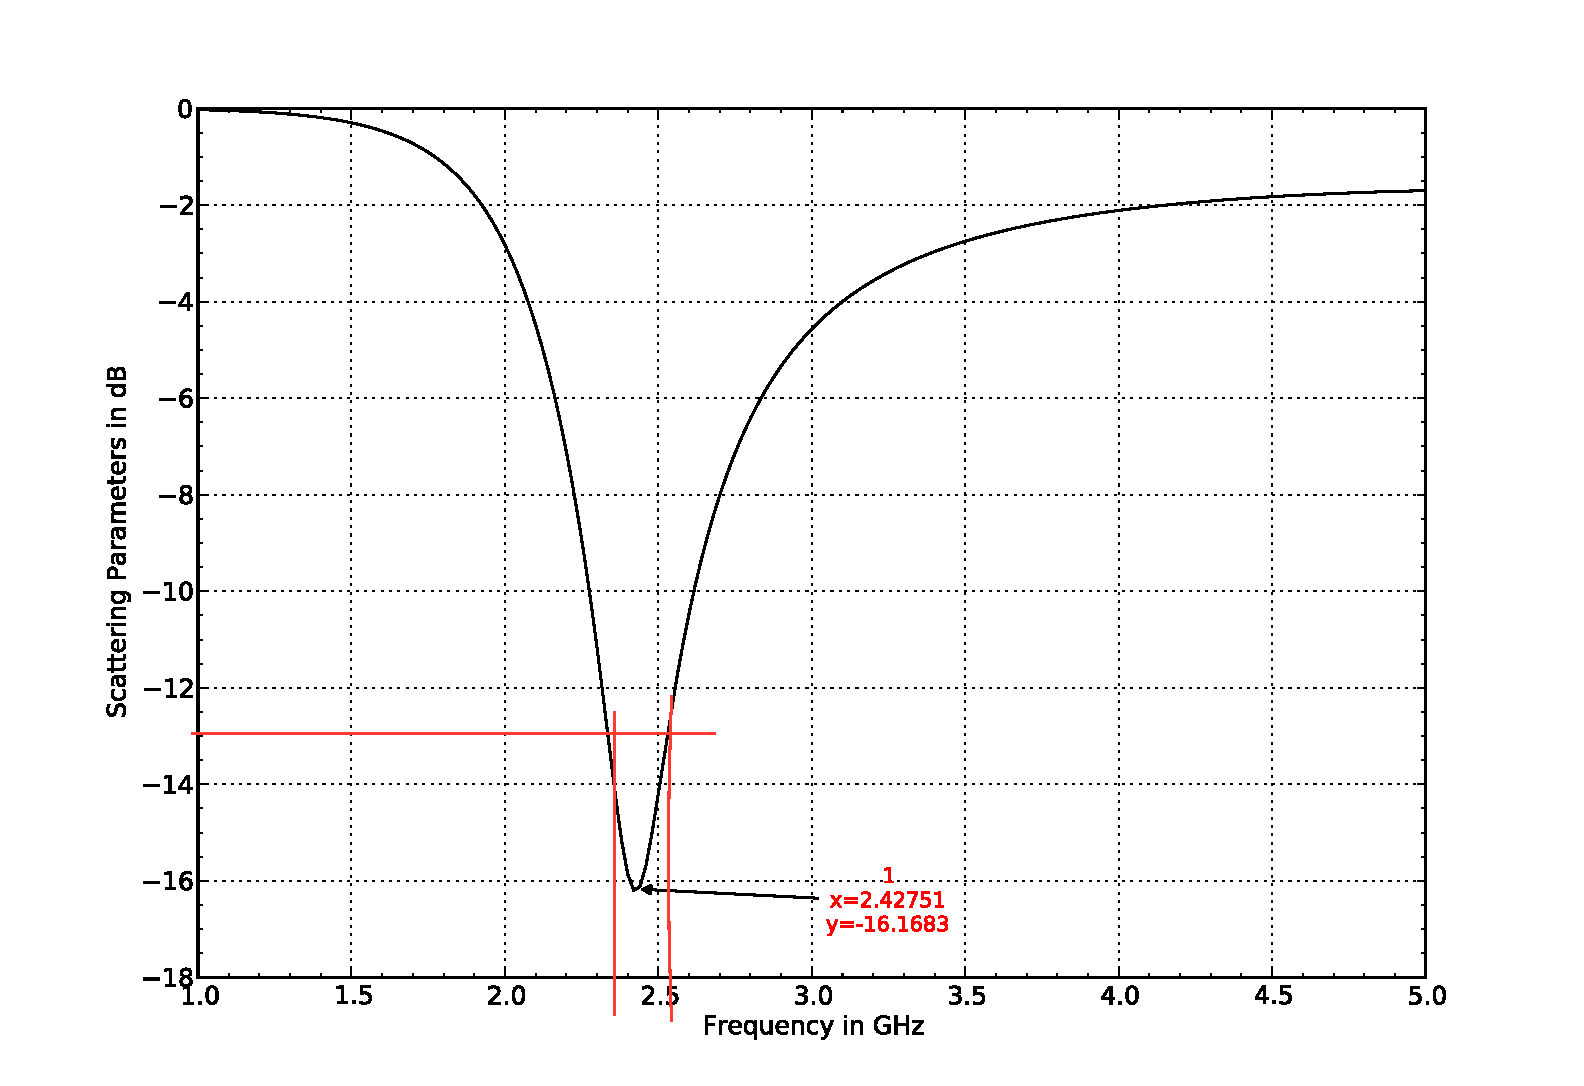
\includegraphics[width=\linewidth]{content/bilder/Evaluation/Dipol/S11DipolOhneABS.pdf}
%  \caption{\\$S_{11}$ Diagramm \\eines Dipols in Freiraum}\label{fig:S11_Dipol_freiraum_1}
%\endminipage%\hfill
%\minipage{0.4\textwidth}
%  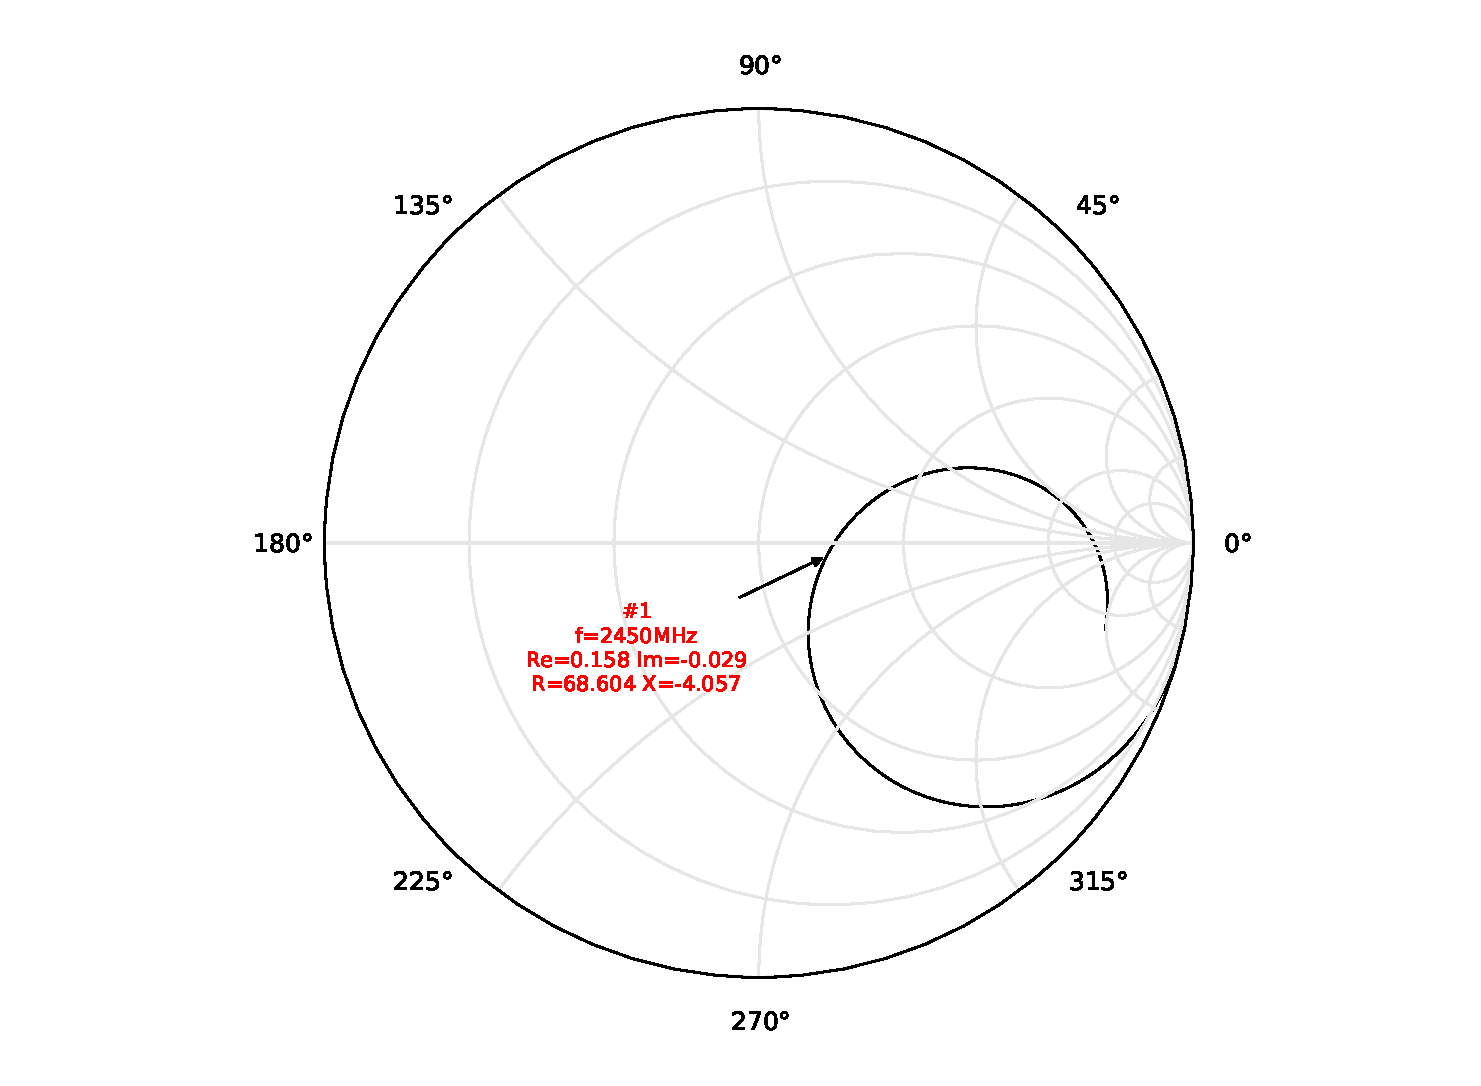
\includegraphics[width=\linewidth]{content/bilder/Evaluation/Dipol/SmithDipolOhneABS.pdf}
%  \caption{\\Smith Diagramm eines Dipols im Freiraum}\label{fig:Smith_Dipol_freiraum_2}
%\endminipage
%\end{center}
%\end{figure}
%\newpage
\textbf{Simulationen einer $\lambda/2$ Dipolantenne mit einem ABS Kunststoffstück im Nahfeld}\\

In der Abbildung \ref{S11_Vergleich_Simulation} wird das $S_{11}$ Diagramm eines Dipols mit einem ABS Kunststoffstück im Nahfeld gezeigt als blaue Kurve dargestellt. Das ABS Stück hat die Masse: 100 x 2 x 30 mm (L x B x H). Es ist direkt an die Antennenstäbe angrenzend. Die dielektrischen Verluste zeigen sich im Detuning der Resonanzfrequenz in der Abbildung \ref{S11_Vergleich_Simulation}. Der maximale $S_{11}$ Wert liegt neu 400 MHz tiefer bei 2.04 GHz. Er zwigt eine Dämpfung von neu -20.79 dB. Die -10dB Bandbreite beträgt 340 MHz.\\

Der Real- und Imaginärteil ist in  Abbildung \ref{Impedanz_Vergleich_Simulation} als grüne und schwarze Kurve gezeigt und macht eine Fehlanpassung deutlich. Bei der Wunschfrequenz von 2.45 GHz entspricht der Realteil der Antennenimpedanz 141 Ohm und der Imaginärteil ist mit $+j39$ Ohm induktiv. Das führt zu einer Abstrahleffizienz $\eta$ von 71.1$\%$.\\
\textbf{Simulationen einer $\lambda/2$ Dipolantenne mit zwei ABS Kunststoffstücken im Nahfeld}\\

Die dritte Simulation zeigt den $S_{11}$ Wert und die Impedanz der Antenne wenn diese zwischen zwei ABS Kunststoffstücken liegt. In der Abbildung \ref{S11_Vergleich_Simulation} ist der $S_{11}$ Wert als grüne Linie gezeichnet.Es zeigt sich dasselbe Verhalten wie bei der Simulation mit nur einem ABS Stück. Die Resonanzfrequenz sinkt weiter ab. Sie liegt neu bei 1.82 GHz und ist somit 180 MHz tiefer als bei der Simulation mit nur einem ABS Stück. Die Abbildung  \ref{S11_Vergleich_Simulation} zeigt weiter, dass die Antenne immer schmalbandiger wird. Die -10dB Bandbreite beträgt 320 MHz.\\
Der Real-und Imaginärteil ist in der Abbildung \ref{Impedanz_Vergleich_Simulation} als gelbe Kurve für den Realteil und als rosa Kurve für den Imaginärteil gekennzeichnet. Sie zeigen eine erhebliche Fehlanpassung an die Referenzquelle. Die Abstrahleffizienz $\eta$ liegt  bei $59.6 \%$. Da die Imedanz $Z_{ant}$ (206.192-j28.979)$\Omega$ bei 2.45GHz entspricht.\\
%\begin{figure}[!h]
%\begin{center}
%\minipage{0.4\textwidth}
%  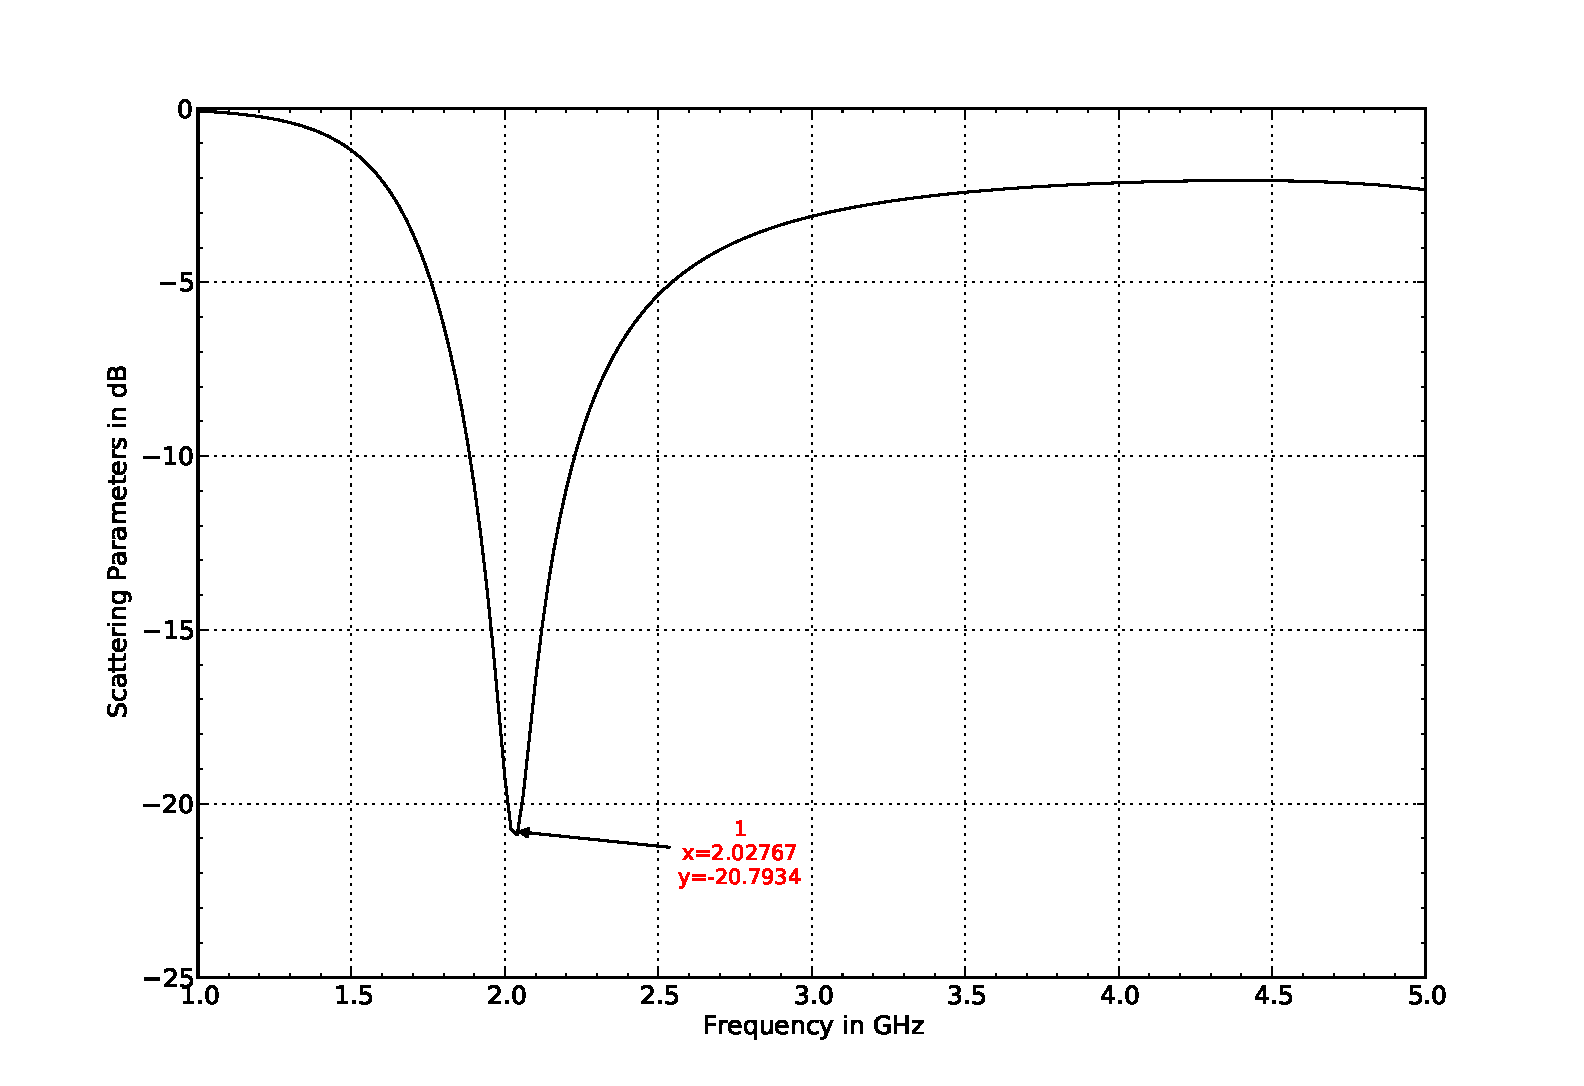
\includegraphics[width=\linewidth]{content/bilder/Evaluation/Dipol/S11DipolABS.pdf}
%  \caption{\\$S_{11}$ eines Dipols mit \\angrenzendem ABS Stück}\label{fig:S11_Dipol_ABS_3}
%\endminipage%\hfill
%\minipage{0.4\textwidth}
%  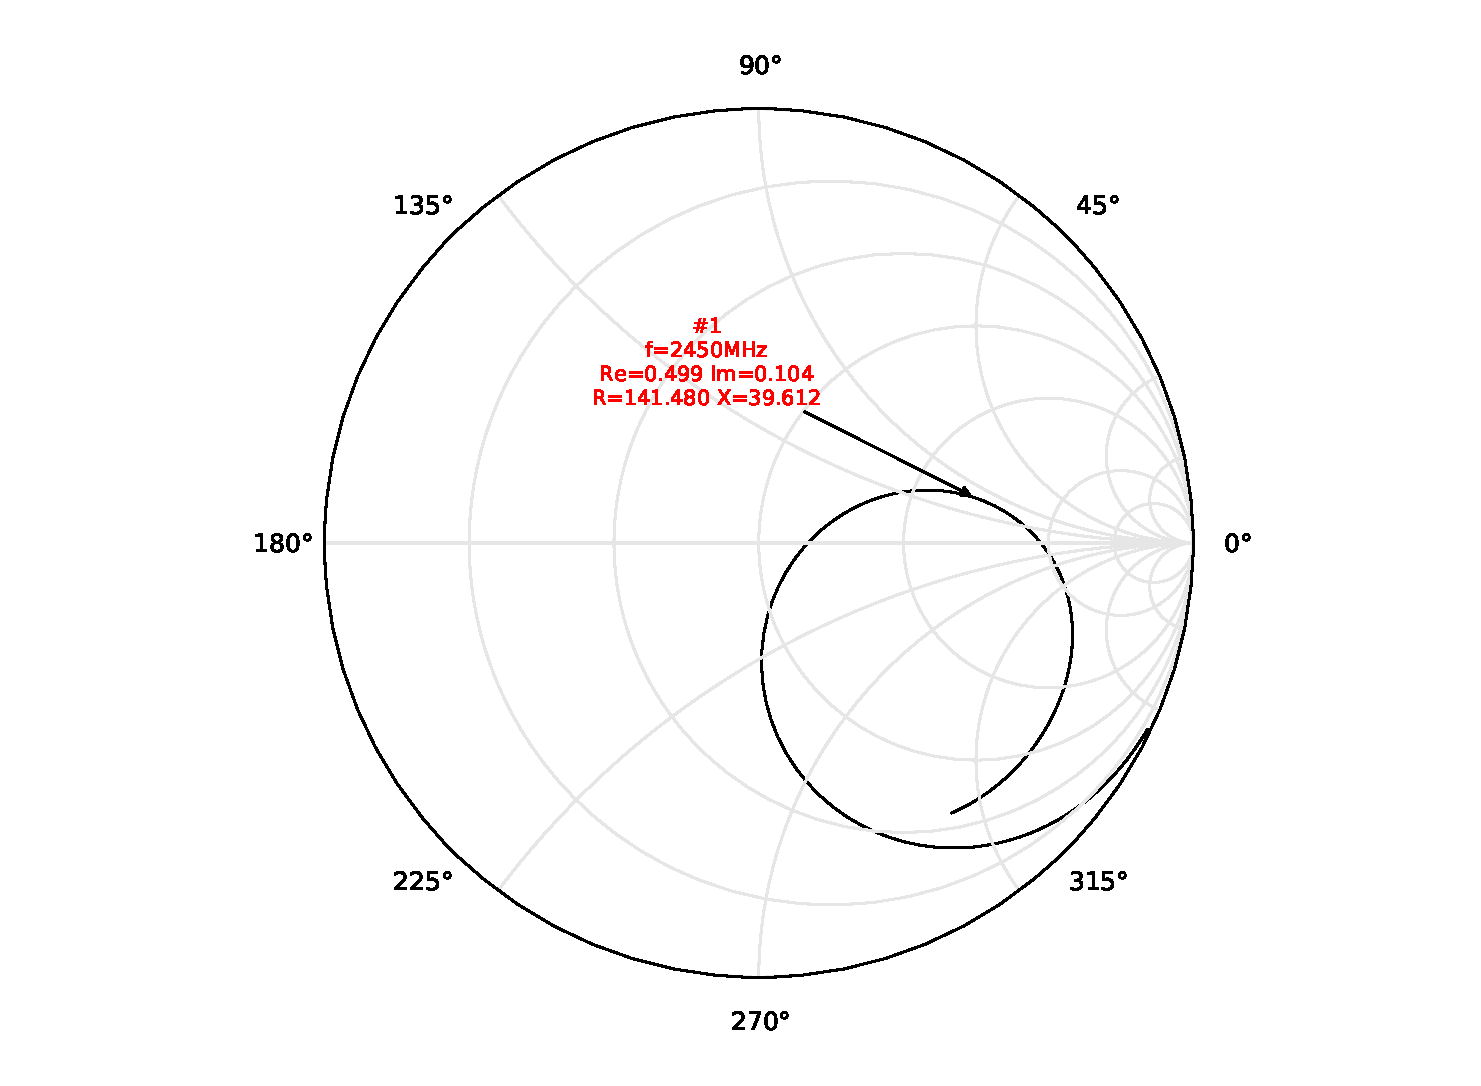
\includegraphics[width=\linewidth]{content/bilder/Evaluation/Dipol/SmithDipolABS.pdf}
%  \caption{\\Smith Diagramm eines Dipols mit angrenzendem ABS Stück}\label{fig:Smith_Dipol_ABS_4}
%\endminipage
%\end{center}
%\end{figure}




%\begin{figure}[!h]
%\begin{center}
%\minipage{0.4\textwidth}
%  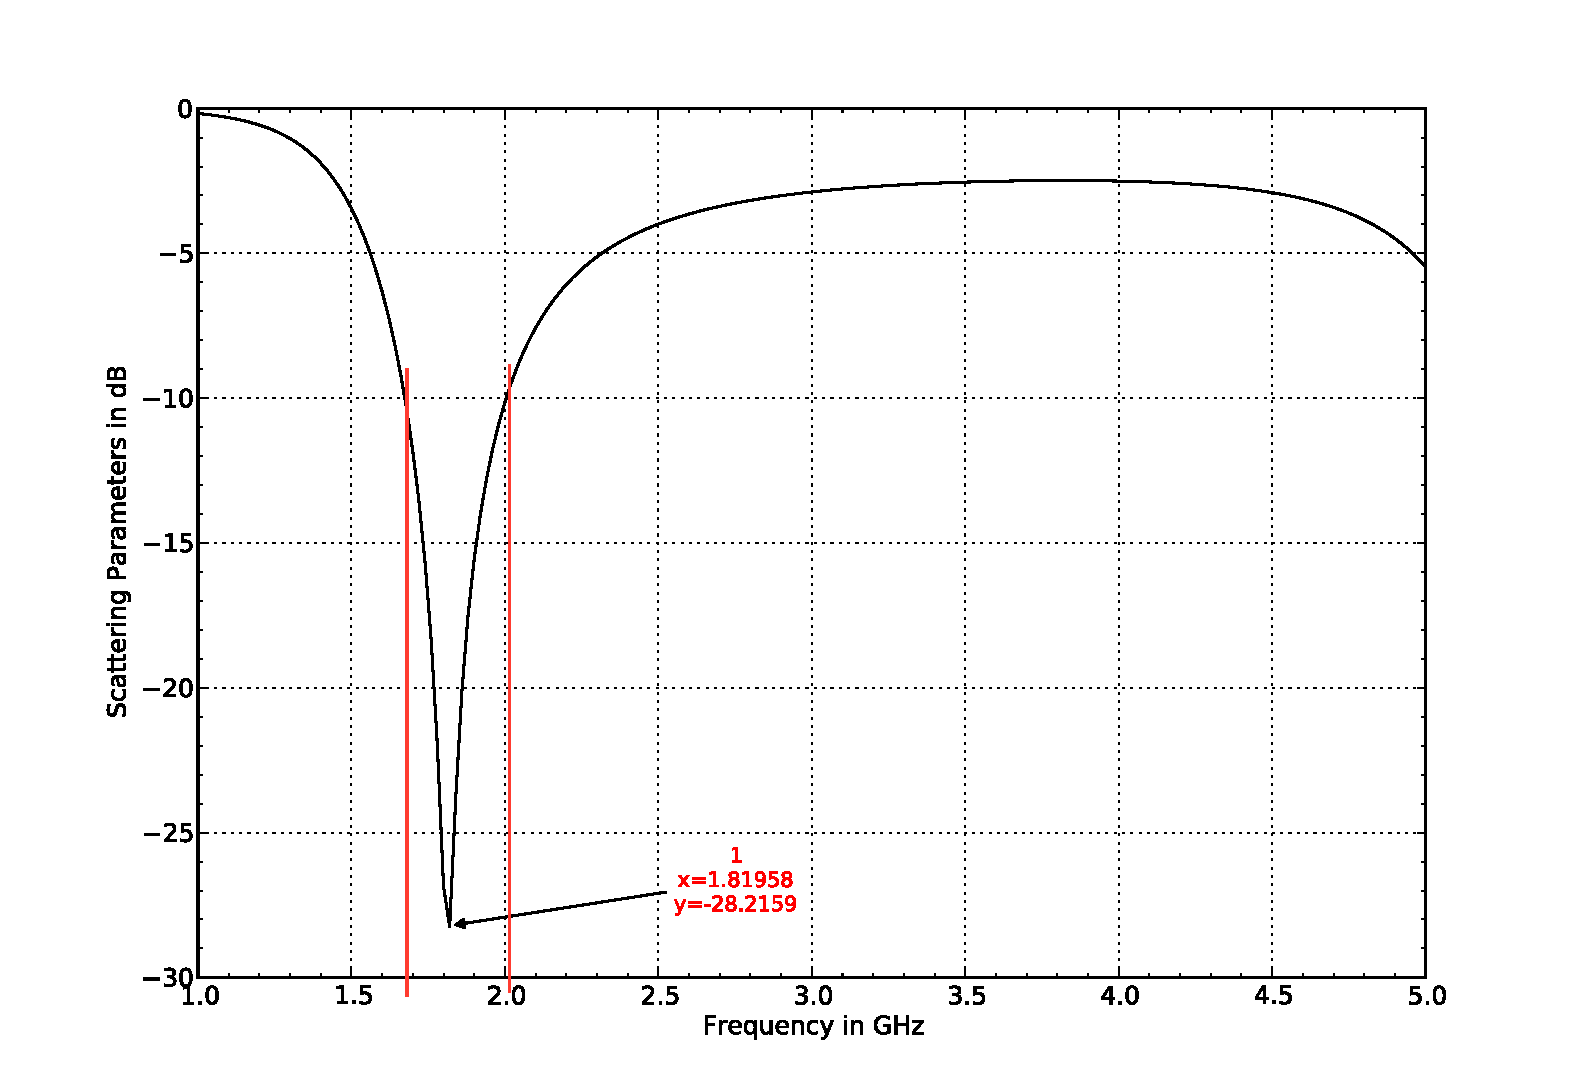
\includegraphics[width=\linewidth]{content/bilder/Evaluation/Dipol/S11DipolZweiABS.pdf}
%  \caption{\\$S_{11}$ eines Dipols zwischen \\zwei ABS Stücken}\label{fig:S11_Dipol_Zwei_ABS_5}
%\endminipage%\hfill
%\minipage{0.4\textwidth}
%  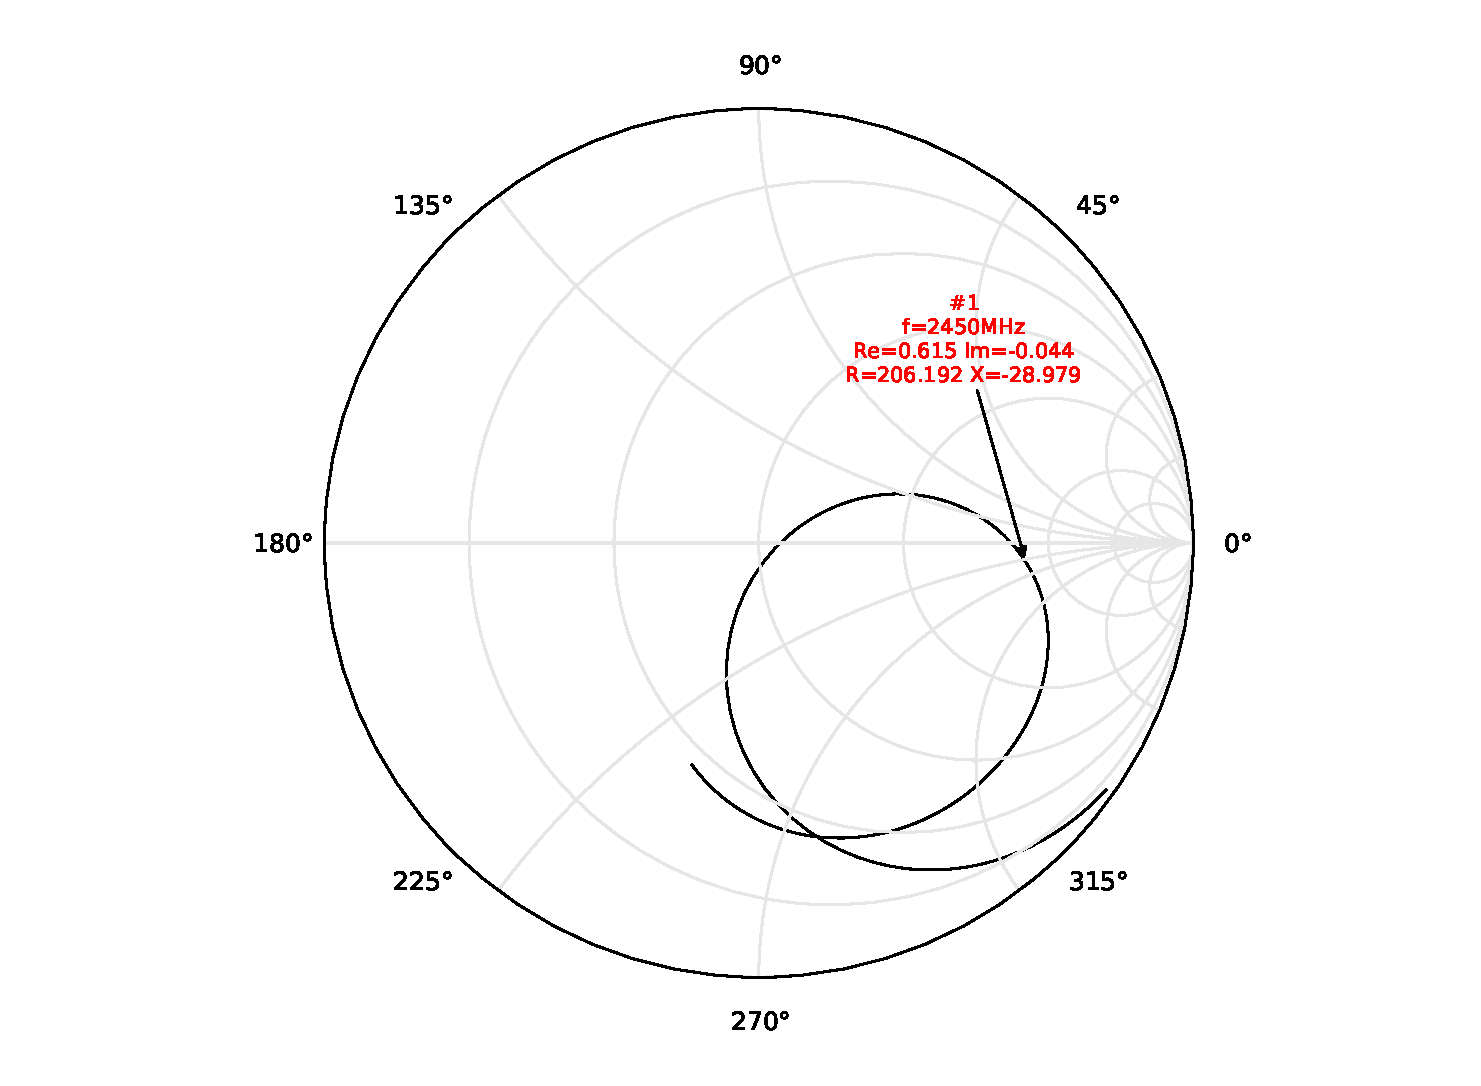
\includegraphics[width=\linewidth]{content/bilder/Evaluation/Dipol/SmithDipolZweiABS.pdf}
%  \caption{\\Smith-Diagramm eines Dipols zwischen zwei ABS Stücken}\label{fig:Smith_Dipol_Zwei_ABS_6}
%\endminipage
%\end{center}
%\end{figure}
Die $|S_{11}|$ Werte der drei Simulationen des $\lambda/2$ Dipols sind in der Grafik \ref{S11_Vergleich_Simulation} gezeigt. Das Detuning ist anhand der nach links laufenden Kurven ersichtlich. Ebenso werden die Kurven schmalbandiger wenn sich Kunststoff im Nahfeld der Antennen befindet.

%%%%%%%%%%%%%%%%%%
\begin{figure}[!ht]
	\centering
	\begingroup
	\inputencoding{latin1}
	% This file was created by matlab2tikz.
%
%The latest updates can be retrieved from
%  http://www.mathworks.com/matlabcentral/fileexchange/22022-matlab2tikz-matlab2tikz
%where you can also make suggestions and rate matlab2tikz.
%
\begin{tikzpicture}

\begin{axis}[%
width=6in,
height=4.5in,
at={(0.758in,0.481in)},
scale only axis,
separate axis lines,
every outer x axis line/.append style={black},
every x tick label/.append style={font=\color{black}},
xmin=1,
xmax=5,
xlabel={Frequenz in [GHz]},
xmajorgrids,
every outer y axis line/.append style={black},
every y tick label/.append style={font=\color{black}},
ymin=-30,
ymax=0,
ylabel={Amplitude in [dB]},
ymajorgrids,
axis background/.style={fill=white},
title={$\text{Simulation des  $|$S}_{\text{11}}\text{$|$ im Freiraum, mit einem und zwei ABS St\"ucken}$},
legend style={at={(0.97,0.03)},anchor=south east,legend cell align=left,align=left,draw=black}
]
\addplot [color=red,very thick,solid]
  table[row sep=crcr]{%
1	-0.0214729\\
1.02	-0.0243143\\
1.04	-0.0274807\\
1.06	-0.0309981\\
1.08	-0.0348949\\
1.1	-0.0392017\\
1.12	-0.0439521\\
1.14	-0.0491826\\
1.16	-0.0549329\\
1.18	-0.0612461\\
1.2	-0.0681692\\
1.22	-0.0757529\\
1.24	-0.0840524\\
1.26	-0.0931273\\
1.28	-0.103043\\
1.3	-0.113869\\
1.32	-0.125684\\
1.34	-0.138572\\
1.36	-0.152626\\
1.38	-0.167947\\
1.4	-0.184647\\
1.42	-0.202851\\
1.44	-0.222692\\
1.46	-0.244319\\
1.48	-0.267898\\
1.5	-0.293606\\
1.52	-0.321643\\
1.54	-0.352227\\
1.56	-0.385597\\
1.58	-0.422017\\
1.6	-0.461778\\
1.62	-0.505203\\
1.64	-0.552646\\
1.66	-0.604498\\
1.68	-0.661194\\
1.7	-0.723211\\
1.72	-0.791078\\
1.74	-0.865379\\
1.76	-0.94676\\
1.78	-1.03593\\
1.8	-1.13368\\
1.82	-1.24086\\
1.84	-1.35843\\
1.86	-1.48744\\
1.88	-1.62904\\
1.9	-1.78448\\
1.92	-1.95516\\
1.94	-2.14258\\
1.96	-2.34839\\
1.98	-2.57442\\
2	-2.82261\\
2.02	-3.09512\\
2.04	-3.39427\\
2.06	-3.72257\\
2.08	-4.08278\\
2.1	-4.47786\\
2.12	-4.91101\\
2.14	-5.38572\\
2.16	-5.90575\\
2.18	-6.47513\\
2.2	-7.09816\\
2.22	-7.7793\\
2.24	-8.52295\\
2.26	-9.33295\\
2.28	-10.2116\\
2.3	-11.1576\\
2.32	-12.1621\\
2.34	-13.2021\\
2.36	-14.2288\\
2.38	-15.1555\\
2.4	-15.8556\\
2.42	-16.1977\\
2.44	-16.1193\\
2.46	-15.6724\\
2.48	-14.984\\
2.5	-14.1814\\
2.52	-13.3537\\
2.54	-12.551\\
2.56	-11.797\\
2.58	-11.1002\\
2.6	-10.4615\\
2.62	-9.87826\\
2.64	-9.34612\\
2.66	-8.86042\\
2.68	-8.41654\\
2.7	-8.01021\\
2.72	-7.63753\\
2.74	-7.29502\\
2.76	-6.97959\\
2.78	-6.6885\\
2.8	-6.41935\\
2.82	-6.17\\
2.84	-5.93856\\
2.86	-5.72335\\
2.88	-5.5229\\
2.9	-5.33587\\
2.92	-5.16109\\
2.94	-4.99752\\
2.96	-4.8442\\
2.98	-4.70029\\
3	-4.56502\\
3.02	-4.43773\\
3.04	-4.31777\\
3.06	-4.2046\\
3.08	-4.09771\\
3.1	-3.99664\\
3.12	-3.90096\\
3.14	-3.81029\\
3.16	-3.72429\\
3.18	-3.64264\\
3.2	-3.56505\\
3.22	-3.49124\\
3.24	-3.42097\\
3.26	-3.35402\\
3.28	-3.29018\\
3.3	-3.22925\\
3.32	-3.17107\\
3.34	-3.11546\\
3.36	-3.06227\\
3.38	-3.01137\\
3.4	-2.96262\\
3.42	-2.9159\\
3.44	-2.8711\\
3.46	-2.82812\\
3.48	-2.78686\\
3.5	-2.74723\\
3.52	-2.70914\\
3.54	-2.67252\\
3.56	-2.63728\\
3.58	-2.60337\\
3.6	-2.57071\\
3.62	-2.53925\\
3.64	-2.50892\\
3.66	-2.47968\\
3.68	-2.45147\\
3.7	-2.42425\\
3.72	-2.39798\\
3.74	-2.3726\\
3.76	-2.34809\\
3.78	-2.32439\\
3.8	-2.30149\\
3.82	-2.27935\\
3.84	-2.25792\\
3.86	-2.2372\\
3.88	-2.21714\\
3.9	-2.19772\\
3.92	-2.17892\\
3.94	-2.1607\\
3.96	-2.14306\\
3.98	-2.12596\\
4	-2.1094\\
4.02	-2.09334\\
4.04	-2.07777\\
4.06	-2.06267\\
4.08	-2.04804\\
4.1	-2.03384\\
4.12	-2.02007\\
4.14	-2.00671\\
4.16	-1.99376\\
4.18	-1.98119\\
4.2	-1.96899\\
4.22	-1.95716\\
4.24	-1.94569\\
4.26	-1.93455\\
4.28	-1.92375\\
4.3	-1.91327\\
4.32	-1.90311\\
4.34	-1.89325\\
4.36	-1.8837\\
4.38	-1.87443\\
4.4	-1.86544\\
4.42	-1.85673\\
4.44	-1.84829\\
4.46	-1.84011\\
4.48	-1.83219\\
4.5	-1.82453\\
4.52	-1.8171\\
4.54	-1.80992\\
4.56	-1.80297\\
4.58	-1.79626\\
4.6	-1.78976\\
4.62	-1.78348\\
4.64	-1.77741\\
4.66	-1.77155\\
4.68	-1.76589\\
4.7	-1.76042\\
4.72	-1.75514\\
4.74	-1.75005\\
4.76	-1.74513\\
4.78	-1.74039\\
4.8	-1.73582\\
4.82	-1.73142\\
4.84	-1.72717\\
4.86	-1.72309\\
4.88	-1.71916\\
4.9	-1.71539\\
4.92	-1.71177\\
4.94	-1.70829\\
4.96	-1.70497\\
4.98	-1.7018\\
5	-1.69878\\
};
\addlegendentry{$\text{S}_{\text{11}}\text{ Frei Raum}$};

\addplot [color=blue,very thick,solid]
  table[row sep=crcr]{%
1	-0.06753\\
1.02	-0.0769903\\
1.04	-0.087552\\
1.06	-0.0993312\\
1.08	-0.112457\\
1.1	-0.127073\\
1.12	-0.143339\\
1.14	-0.161434\\
1.16	-0.181556\\
1.18	-0.203927\\
1.2	-0.228795\\
1.22	-0.256438\\
1.24	-0.287165\\
1.26	-0.321325\\
1.28	-0.359307\\
1.3	-0.401547\\
1.32	-0.448535\\
1.34	-0.500819\\
1.36	-0.559015\\
1.38	-0.623814\\
1.4	-0.695992\\
1.42	-0.776418\\
1.44	-0.866069\\
1.46	-0.966038\\
1.48	-1.07755\\
1.5	-1.20197\\
1.52	-1.34084\\
1.54	-1.49587\\
1.56	-1.66896\\
1.58	-1.86223\\
1.6	-2.07805\\
1.62	-2.31902\\
1.64	-2.58807\\
1.66	-2.88839\\
1.68	-3.22355\\
1.7	-3.59752\\
1.72	-4.0147\\
1.74	-4.48004\\
1.76	-4.99912\\
1.78	-5.57832\\
1.8	-6.22501\\
1.82	-6.94791\\
1.84	-7.75744\\
1.86	-8.66635\\
1.88	-9.69045\\
1.9	-10.8495\\
1.92	-12.1678\\
1.94	-13.6732\\
1.96	-15.3895\\
1.98	-17.3042\\
2	-19.2615\\
2.02	-20.7304\\
2.04	-20.8947\\
2.06	-19.7393\\
2.08	-18.0739\\
2.1	-16.4378\\
2.12	-14.9906\\
2.14	-13.744\\
2.16	-12.6728\\
2.18	-11.7475\\
2.2	-10.9424\\
2.22	-10.2365\\
2.24	-9.61322\\
2.26	-9.05946\\
2.28	-8.56463\\
2.3	-8.12018\\
2.32	-7.71913\\
2.34	-7.35574\\
2.36	-7.02521\\
2.38	-6.72354\\
2.4	-6.44732\\
2.42	-6.19367\\
2.44	-5.96011\\
2.46	-5.74449\\
2.48	-5.54498\\
2.5	-5.35995\\
2.52	-5.18801\\
2.54	-5.0279\\
2.56	-4.87854\\
2.58	-4.73896\\
2.6	-4.6083\\
2.62	-4.48581\\
2.64	-4.37079\\
2.66	-4.26264\\
2.68	-4.16081\\
2.7	-4.0648\\
2.72	-3.97417\\
2.74	-3.88852\\
2.76	-3.80748\\
2.78	-3.73072\\
2.8	-3.65794\\
2.82	-3.58886\\
2.84	-3.52323\\
2.86	-3.46082\\
2.88	-3.40142\\
2.9	-3.34484\\
2.92	-3.29091\\
2.94	-3.23945\\
2.96	-3.19032\\
2.98	-3.14337\\
3	-3.09849\\
3.02	-3.05554\\
3.04	-3.01443\\
3.06	-2.97504\\
3.08	-2.93729\\
3.1	-2.90109\\
3.12	-2.86635\\
3.14	-2.83299\\
3.16	-2.80096\\
3.18	-2.77017\\
3.2	-2.74057\\
3.22	-2.71211\\
3.24	-2.68472\\
3.26	-2.65835\\
3.28	-2.63297\\
3.3	-2.60851\\
3.32	-2.58495\\
3.34	-2.56224\\
3.36	-2.54035\\
3.38	-2.51924\\
3.4	-2.49887\\
3.42	-2.47923\\
3.44	-2.46028\\
3.46	-2.44198\\
3.48	-2.42433\\
3.5	-2.40729\\
3.52	-2.39084\\
3.54	-2.37497\\
3.56	-2.35964\\
3.58	-2.34484\\
3.6	-2.33056\\
3.62	-2.31678\\
3.64	-2.30348\\
3.66	-2.29065\\
3.68	-2.27828\\
3.7	-2.26635\\
3.72	-2.25485\\
3.74	-2.24377\\
3.76	-2.23309\\
3.78	-2.22282\\
3.8	-2.21294\\
3.82	-2.20343\\
3.84	-2.1943\\
3.86	-2.18553\\
3.88	-2.17712\\
3.9	-2.16905\\
3.92	-2.16132\\
3.94	-2.15391\\
3.96	-2.14683\\
3.98	-2.14007\\
4	-2.13361\\
4.02	-2.12745\\
4.04	-2.12158\\
4.06	-2.11602\\
4.08	-2.11074\\
4.1	-2.10575\\
4.12	-2.10106\\
4.14	-2.09666\\
4.16	-2.09255\\
4.18	-2.08875\\
4.2	-2.08524\\
4.22	-2.08205\\
4.24	-2.07917\\
4.26	-2.07661\\
4.28	-2.07437\\
4.3	-2.07246\\
4.32	-2.07089\\
4.34	-2.06967\\
4.36	-2.06881\\
4.38	-2.0683\\
4.4	-2.06817\\
4.42	-2.06843\\
4.44	-2.06907\\
4.46	-2.07012\\
4.48	-2.0716\\
4.5	-2.0735\\
4.52	-2.07586\\
4.54	-2.07868\\
4.56	-2.08199\\
4.58	-2.08579\\
4.6	-2.09012\\
4.62	-2.095\\
4.64	-2.10045\\
4.66	-2.10649\\
4.68	-2.11316\\
4.7	-2.12049\\
4.72	-2.1285\\
4.74	-2.13724\\
4.76	-2.14675\\
4.78	-2.15705\\
4.8	-2.1682\\
4.82	-2.18024\\
4.84	-2.19324\\
4.86	-2.20723\\
4.88	-2.22229\\
4.9	-2.23847\\
4.92	-2.25585\\
4.94	-2.2745\\
4.96	-2.29449\\
4.98	-2.31593\\
5	-2.33889\\
};
\addlegendentry{$\text{S}_{\text{11}}\text{ mit ABS}$};

\addplot [color=green,very thick,solid]
  table[row sep=crcr]{%
1	-0.168213\\
1.02	-0.190447\\
1.04	-0.215463\\
1.06	-0.243599\\
1.08	-0.275239\\
1.1	-0.310818\\
1.12	-0.350826\\
1.14	-0.395823\\
1.16	-0.446441\\
1.18	-0.503401\\
1.2	-0.567518\\
1.22	-0.639721\\
1.24	-0.721062\\
1.26	-0.81274\\
1.28	-0.916112\\
1.3	-1.03272\\
1.32	-1.1643\\
1.34	-1.31285\\
1.36	-1.48058\\
1.38	-1.67001\\
1.4	-1.88399\\
1.42	-2.12571\\
1.44	-2.39874\\
1.46	-2.70711\\
1.48	-3.05535\\
1.5	-3.44853\\
1.52	-3.8924\\
1.54	-4.39351\\
1.56	-4.95941\\
1.58	-5.59896\\
1.6	-6.32276\\
1.62	-7.14388\\
1.64	-8.079\\
1.66	-9.15016\\
1.68	-10.3878\\
1.7	-11.8361\\
1.72	-13.5627\\
1.74	-15.6782\\
1.76	-18.3768\\
1.78	-22.0109\\
1.8	-26.8533\\
1.82	-28.2448\\
1.84	-23.7602\\
1.86	-20.097\\
1.88	-17.496\\
1.9	-15.5493\\
1.92	-14.023\\
1.94	-12.7854\\
1.96	-11.7571\\
1.98	-10.8867\\
2	-10.1394\\
2.02	-9.49037\\
2.04	-8.92137\\
2.06	-8.41859\\
2.08	-7.97132\\
2.1	-7.57112\\
2.12	-7.21121\\
2.14	-6.88605\\
2.16	-6.59109\\
2.18	-6.32255\\
2.2	-6.07724\\
2.22	-5.85245\\
2.24	-5.6459\\
2.26	-5.4556\\
2.28	-5.27985\\
2.3	-5.11717\\
2.32	-4.96626\\
2.34	-4.826\\
2.36	-4.6954\\
2.38	-4.57356\\
2.4	-4.45973\\
2.42	-4.3532\\
2.44	-4.25336\\
2.46	-4.15966\\
2.48	-4.0716\\
2.5	-3.98874\\
2.52	-3.91068\\
2.54	-3.83706\\
2.56	-3.76755\\
2.58	-3.70186\\
2.6	-3.63971\\
2.62	-3.58087\\
2.64	-3.5251\\
2.66	-3.47221\\
2.68	-3.422\\
2.7	-3.3743\\
2.72	-3.32896\\
2.74	-3.28583\\
2.76	-3.24478\\
2.78	-3.20568\\
2.8	-3.16843\\
2.82	-3.13291\\
2.84	-3.09903\\
2.86	-3.0667\\
2.88	-3.03584\\
2.9	-3.00636\\
2.92	-2.9782\\
2.94	-2.9513\\
2.96	-2.92557\\
2.98	-2.90098\\
3	-2.87747\\
3.02	-2.85497\\
3.04	-2.83346\\
3.06	-2.81289\\
3.08	-2.7932\\
3.1	-2.77438\\
3.12	-2.75637\\
3.14	-2.73915\\
3.16	-2.72269\\
3.18	-2.70695\\
3.2	-2.69191\\
3.22	-2.67756\\
3.24	-2.66385\\
3.26	-2.65077\\
3.28	-2.63831\\
3.3	-2.62644\\
3.32	-2.61514\\
3.34	-2.6044\\
3.36	-2.5942\\
3.38	-2.58453\\
3.4	-2.57537\\
3.42	-2.5667\\
3.44	-2.55852\\
3.46	-2.5508\\
3.48	-2.54353\\
3.5	-2.53669\\
3.52	-2.53028\\
3.54	-2.52428\\
3.56	-2.51868\\
3.58	-2.51347\\
3.6	-2.50865\\
3.62	-2.50422\\
3.64	-2.50018\\
3.66	-2.49653\\
3.68	-2.49328\\
3.7	-2.49043\\
3.72	-2.48799\\
3.74	-2.48597\\
3.76	-2.48436\\
3.78	-2.48318\\
3.8	-2.48243\\
3.82	-2.48213\\
3.84	-2.48228\\
3.86	-2.48289\\
3.88	-2.48397\\
3.9	-2.48553\\
3.92	-2.48759\\
3.94	-2.49016\\
3.96	-2.49326\\
3.98	-2.49689\\
4	-2.50109\\
4.02	-2.50587\\
4.04	-2.51125\\
4.06	-2.51726\\
4.08	-2.52393\\
4.1	-2.53129\\
4.12	-2.53936\\
4.14	-2.54819\\
4.16	-2.5578\\
4.18	-2.56825\\
4.2	-2.57958\\
4.22	-2.59184\\
4.24	-2.60507\\
4.26	-2.61934\\
4.28	-2.63472\\
4.3	-2.65125\\
4.32	-2.66903\\
4.34	-2.68814\\
4.36	-2.70865\\
4.38	-2.73066\\
4.4	-2.75427\\
4.42	-2.77961\\
4.44	-2.80678\\
4.46	-2.83593\\
4.48	-2.8672\\
4.5	-2.90074\\
4.52	-2.93672\\
4.54	-2.97534\\
4.56	-3.0168\\
4.58	-3.06133\\
4.6	-3.10916\\
4.62	-3.16058\\
4.64	-3.21586\\
4.66	-3.27534\\
4.68	-3.33937\\
4.7	-3.40833\\
4.72	-3.48265\\
4.74	-3.56281\\
4.76	-3.6493\\
4.78	-3.7427\\
4.8	-3.84364\\
4.82	-3.95278\\
4.84	-4.0709\\
4.86	-4.19881\\
4.88	-4.33745\\
4.9	-4.48782\\
4.92	-4.65104\\
4.94	-4.82835\\
4.96	-5.02113\\
4.98	-5.23089\\
5	-5.45933\\
};
\addlegendentry{$\text{S}_{\text{11}}\text{ mit 2 ABS}$};

\end{axis}
\end{tikzpicture}%
	\endgroup
	\caption{Vergleich des $S_{11}$}
	\label{S11_Vergleich_Simulation}
\end{figure}
%%%%%%%%%%%%%%%%%%%%%%%%%%%%%%%%%%%%%%%%%%%%%%%%%%%%%%%
\newpage
Die Antennenimpedanz aller drei Simulationen sind in der folgenden Abbildung \ref{Impedanz_Vergleich_Simulation} dargestellt. Jede der drei Impedanzen wird mit einer Kurve für den Realteil und den Imaginärteil dargestellt. 
\begin{figure}[!ht]
	\centering
	\begingroup
	\inputencoding{latin1}
	% This file was created by matlab2tikz.
%
%The latest updates can be retrieved from
%  http://www.mathworks.com/matlabcentral/fileexchange/22022-matlab2tikz-matlab2tikz
%where you can also make suggestions and rate matlab2tikz.
%
\definecolor{mycolor1}{rgb}{1.00000,1.00000,0.00000}%
\definecolor{mycolor2}{rgb}{1.00000,0.00000,1.00000}%
%
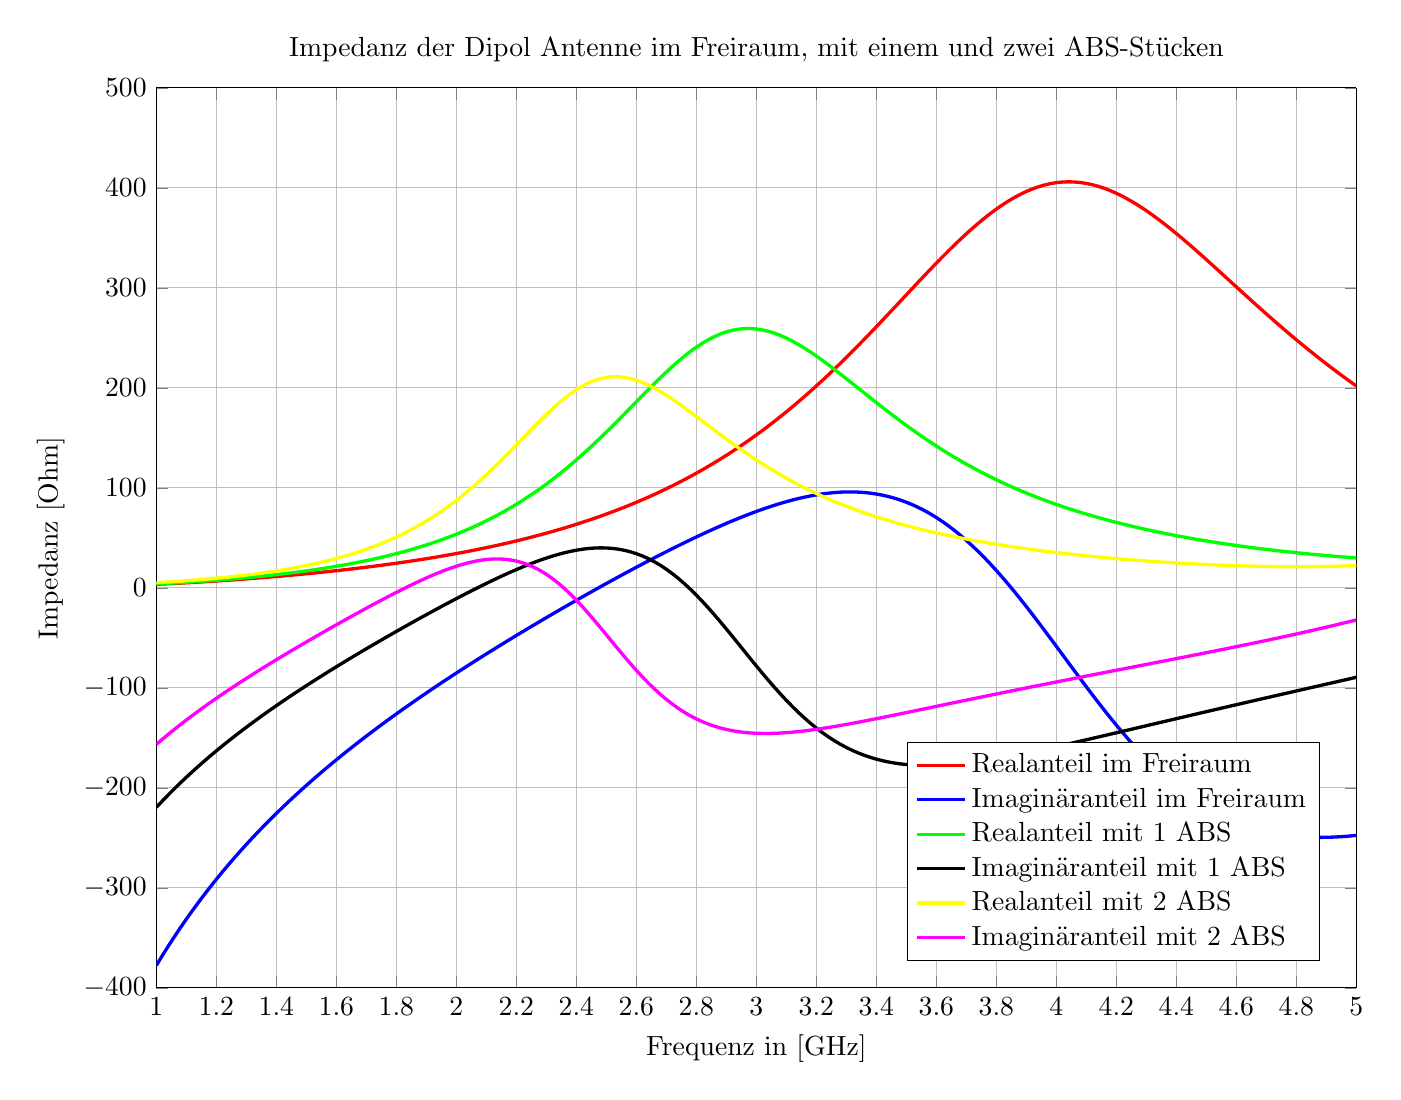
\begin{tikzpicture}

\begin{axis}[%
width=6in,
height=4.5in,
at={(0.758in,0.481in)},
scale only axis,
separate axis lines,
every outer x axis line/.append style={black},
every x tick label/.append style={font=\color{black}},
xmin=1,
xmax=5,
xlabel={Frequenz in [GHz]},
xmajorgrids,
every outer y axis line/.append style={black},
every y tick label/.append style={font=\color{black}},
ymin=-400,
ymax=500,
ylabel={Impedanz [Ohm]},
ymajorgrids,
axis background/.style={fill=white},
title={Impedanz der Dipol Antenne im Freiraum, mit einem und zwei ABS-Stücken},
legend style={at={(0.97,0.03)},anchor=south east,legend cell align=left,align=left,draw=black}
]
\addplot [color=red,very thick,solid]
  table[row sep=crcr]{%
1	3.58549\\
1.02	3.85403\\
1.04	4.13672\\
1.06	4.43305\\
1.08	4.74263\\
1.1	5.0651\\
1.12	5.4002\\
1.14	5.74775\\
1.16	6.1076\\
1.18	6.47966\\
1.2	6.86384\\
1.22	7.26011\\
1.24	7.66841\\
1.26	8.08872\\
1.28	8.52102\\
1.3	8.96531\\
1.32	9.42162\\
1.34	9.89004\\
1.36	10.3707\\
1.38	10.8637\\
1.4	11.3693\\
1.42	11.8877\\
1.44	12.4191\\
1.46	12.964\\
1.48	13.5227\\
1.5	14.0953\\
1.52	14.6825\\
1.54	15.2844\\
1.56	15.9015\\
1.58	16.5341\\
1.6	17.1827\\
1.62	17.8477\\
1.64	18.5295\\
1.66	19.2286\\
1.68	19.9455\\
1.7	20.6808\\
1.72	21.4349\\
1.74	22.2084\\
1.76	23.002\\
1.78	23.8162\\
1.8	24.6516\\
1.82	25.509\\
1.84	26.3889\\
1.86	27.292\\
1.88	28.219\\
1.9	29.1706\\
1.92	30.1475\\
1.94	31.1506\\
1.96	32.1804\\
1.98	33.238\\
2	34.3241\\
2.02	35.4395\\
2.04	36.5853\\
2.06	37.7622\\
2.08	38.9714\\
2.1	40.2137\\
2.12	41.4901\\
2.14	42.8018\\
2.16	44.1496\\
2.18	45.5349\\
2.2	46.9585\\
2.22	48.4218\\
2.24	49.9259\\
2.26	51.472\\
2.28	53.0615\\
2.3	54.6955\\
2.32	56.3756\\
2.34	58.103\\
2.36	59.8793\\
2.38	61.7059\\
2.4	63.5842\\
2.42	65.5159\\
2.44	67.5026\\
2.46	69.5458\\
2.48	71.6472\\
2.5	73.8086\\
2.52	76.0316\\
2.54	78.3181\\
2.56	80.6698\\
2.58	83.0888\\
2.6	85.5768\\
2.62	88.1358\\
2.64	90.7677\\
2.66	93.4747\\
2.68	96.2587\\
2.7	99.1218\\
2.72	102.066\\
2.74	105.094\\
2.76	108.206\\
2.78	111.407\\
2.8	114.696\\
2.82	118.078\\
2.84	121.553\\
2.86	125.123\\
2.88	128.791\\
2.9	132.559\\
2.92	136.428\\
2.94	140.4\\
2.96	144.478\\
2.98	148.661\\
3	152.953\\
3.02	157.353\\
3.04	161.863\\
3.06	166.485\\
3.08	171.218\\
3.1	176.063\\
3.12	181.02\\
3.14	186.089\\
3.16	191.269\\
3.18	196.558\\
3.2	201.957\\
3.22	207.461\\
3.24	213.07\\
3.26	218.78\\
3.28	224.588\\
3.3	230.488\\
3.32	236.476\\
3.34	242.546\\
3.36	248.692\\
3.38	254.907\\
3.4	261.181\\
3.42	267.506\\
3.44	273.873\\
3.46	280.269\\
3.48	286.683\\
3.5	293.103\\
3.52	299.514\\
3.54	305.902\\
3.56	312.25\\
3.58	318.544\\
3.6	324.765\\
3.62	330.895\\
3.64	336.916\\
3.66	342.809\\
3.68	348.553\\
3.7	354.13\\
3.72	359.52\\
3.74	364.701\\
3.76	369.655\\
3.78	374.362\\
3.8	378.803\\
3.82	382.961\\
3.84	386.817\\
3.86	390.356\\
3.88	393.563\\
3.9	396.425\\
3.92	398.93\\
3.94	401.068\\
3.96	402.832\\
3.98	404.214\\
4	405.211\\
4.02	405.822\\
4.04	406.045\\
4.06	405.883\\
4.08	405.341\\
4.1	404.424\\
4.12	403.139\\
4.14	401.498\\
4.16	399.511\\
4.18	397.19\\
4.2	394.55\\
4.22	391.606\\
4.24	388.374\\
4.26	384.872\\
4.28	381.116\\
4.3	377.124\\
4.32	372.916\\
4.34	368.509\\
4.36	363.922\\
4.38	359.172\\
4.4	354.279\\
4.42	349.258\\
4.44	344.127\\
4.46	338.903\\
4.48	333.601\\
4.5	328.237\\
4.52	322.824\\
4.54	317.376\\
4.56	311.906\\
4.58	306.427\\
4.6	300.948\\
4.62	295.482\\
4.64	290.035\\
4.66	284.619\\
4.68	279.239\\
4.7	273.903\\
4.72	268.617\\
4.74	263.386\\
4.76	258.215\\
4.78	253.108\\
4.8	248.069\\
4.82	243.101\\
4.84	238.206\\
4.86	233.386\\
4.88	228.642\\
4.9	223.977\\
4.92	219.39\\
4.94	214.882\\
4.96	210.453\\
4.98	206.104\\
5	201.835\\
};
\addlegendentry{Realanteil im Freiraum};

\addplot [color=blue,very thick,solid]
  table[row sep=crcr]{%
1	-377.521\\
1.02	-367.647\\
1.04	-358.097\\
1.06	-348.853\\
1.08	-339.897\\
1.1	-331.213\\
1.12	-322.787\\
1.14	-314.605\\
1.16	-306.653\\
1.18	-298.921\\
1.2	-291.396\\
1.22	-284.068\\
1.24	-276.927\\
1.26	-269.963\\
1.28	-263.169\\
1.3	-256.536\\
1.32	-250.055\\
1.34	-243.72\\
1.36	-237.524\\
1.38	-231.46\\
1.4	-225.522\\
1.42	-219.704\\
1.44	-214\\
1.46	-208.406\\
1.48	-202.916\\
1.5	-197.525\\
1.52	-192.229\\
1.54	-187.025\\
1.56	-181.907\\
1.58	-176.872\\
1.6	-171.916\\
1.62	-167.037\\
1.64	-162.23\\
1.66	-157.493\\
1.68	-152.822\\
1.7	-148.215\\
1.72	-143.669\\
1.74	-139.181\\
1.76	-134.749\\
1.78	-130.37\\
1.8	-126.043\\
1.82	-121.765\\
1.84	-117.534\\
1.86	-113.348\\
1.88	-109.205\\
1.9	-105.104\\
1.92	-101.043\\
1.94	-97.0207\\
1.96	-93.0347\\
1.98	-89.084\\
2	-85.1672\\
2.02	-81.283\\
2.04	-77.4302\\
2.06	-73.6075\\
2.08	-69.8139\\
2.1	-66.0483\\
2.12	-62.3099\\
2.14	-58.5977\\
2.16	-54.9108\\
2.18	-51.2485\\
2.2	-47.6102\\
2.22	-43.9951\\
2.24	-40.4026\\
2.26	-36.8323\\
2.28	-33.2836\\
2.3	-29.7562\\
2.32	-26.2498\\
2.34	-22.7641\\
2.36	-19.299\\
2.38	-15.8543\\
2.4	-12.4302\\
2.42	-9.02656\\
2.44	-5.64368\\
2.46	-2.28179\\
2.48	1.05879\\
2.5	4.37762\\
2.52	7.67418\\
2.54	10.9478\\
2.56	14.1979\\
2.58	17.4234\\
2.6	20.6235\\
2.62	23.797\\
2.64	26.9427\\
2.66	30.0592\\
2.68	33.1451\\
2.7	36.1985\\
2.72	39.2178\\
2.74	42.2008\\
2.76	45.1455\\
2.78	48.0493\\
2.8	50.9099\\
2.82	53.7244\\
2.84	56.4899\\
2.86	59.2031\\
2.88	61.8607\\
2.9	64.459\\
2.92	66.9942\\
2.94	69.462\\
2.96	71.858\\
2.98	74.1775\\
3	76.4156\\
3.02	78.567\\
3.04	80.626\\
3.06	82.587\\
3.08	84.4436\\
3.1	86.1895\\
3.12	87.8178\\
3.14	89.3215\\
3.16	90.6932\\
3.18	91.9252\\
3.2	93.0097\\
3.22	93.9384\\
3.24	94.7028\\
3.26	95.2944\\
3.28	95.7042\\
3.3	95.9232\\
3.32	95.9423\\
3.34	95.7523\\
3.36	95.3439\\
3.38	94.7078\\
3.4	93.8351\\
3.42	92.7166\\
3.44	91.3438\\
3.46	89.7082\\
3.48	87.8021\\
3.5	85.6178\\
3.52	83.1487\\
3.54	80.3888\\
3.56	77.3329\\
3.58	73.9767\\
3.6	70.3171\\
3.62	66.3522\\
3.64	62.0811\\
3.66	57.5047\\
3.68	52.625\\
3.7	47.4458\\
3.72	41.9725\\
3.74	36.2122\\
3.76	30.1737\\
3.78	23.8676\\
3.8	17.3061\\
3.82	10.5033\\
3.84	3.47482\\
3.86	-3.76198\\
3.88	-11.1884\\
3.9	-18.7843\\
3.92	-26.5285\\
3.94	-34.3984\\
3.96	-42.371\\
3.98	-50.4222\\
4	-58.5277\\
4.02	-66.6629\\
4.04	-74.8031\\
4.06	-82.9238\\
4.08	-91.001\\
4.1	-99.0111\\
4.12	-106.931\\
4.14	-114.74\\
4.16	-122.417\\
4.18	-129.942\\
4.2	-137.298\\
4.22	-144.467\\
4.24	-151.436\\
4.26	-158.19\\
4.28	-164.718\\
4.3	-171.01\\
4.32	-177.057\\
4.34	-182.852\\
4.36	-188.391\\
4.38	-193.668\\
4.4	-198.683\\
4.42	-203.432\\
4.44	-207.918\\
4.46	-212.14\\
4.48	-216.101\\
4.5	-219.803\\
4.52	-223.252\\
4.54	-226.452\\
4.56	-229.409\\
4.58	-232.128\\
4.6	-234.616\\
4.62	-236.881\\
4.64	-238.929\\
4.66	-240.769\\
4.68	-242.409\\
4.7	-243.856\\
4.72	-245.118\\
4.74	-246.204\\
4.76	-247.121\\
4.78	-247.876\\
4.8	-248.478\\
4.82	-248.933\\
4.84	-249.25\\
4.86	-249.434\\
4.88	-249.492\\
4.9	-249.431\\
4.92	-249.257\\
4.94	-248.975\\
4.96	-248.591\\
4.98	-248.109\\
5	-247.535\\
};
\addlegendentry{Imagin\"aranteil im Freiraum};

\addplot [color=green,very thick,solid]
  table[row sep=crcr]{%
1	3.93961\\
1.02	4.24702\\
1.04	4.56779\\
1.06	4.90227\\
1.08	5.25088\\
1.1	5.61404\\
1.12	5.99225\\
1.14	6.38601\\
1.16	6.79588\\
1.18	7.22246\\
1.2	7.66639\\
1.22	8.12836\\
1.24	8.60908\\
1.26	9.10931\\
1.28	9.62988\\
1.3	10.1716\\
1.32	10.7354\\
1.34	11.3223\\
1.36	11.9331\\
1.38	12.5691\\
1.4	13.2312\\
1.42	13.9206\\
1.44	14.6385\\
1.46	15.3862\\
1.48	16.1651\\
1.5	16.9765\\
1.52	17.822\\
1.54	18.7029\\
1.56	19.621\\
1.58	20.578\\
1.6	21.5757\\
1.62	22.6158\\
1.64	23.7004\\
1.66	24.8315\\
1.68	26.0113\\
1.7	27.242\\
1.72	28.526\\
1.74	29.8658\\
1.76	31.2639\\
1.78	32.723\\
1.8	34.246\\
1.82	35.8359\\
1.84	37.4957\\
1.86	39.2286\\
1.88	41.038\\
1.9	42.9274\\
1.92	44.9004\\
1.94	46.9608\\
1.96	49.1124\\
1.98	51.3593\\
2	53.7055\\
2.02	56.1555\\
2.04	58.7134\\
2.06	61.3837\\
2.08	64.1709\\
2.1	67.0796\\
2.12	70.1143\\
2.14	73.2796\\
2.16	76.5798\\
2.18	80.0195\\
2.2	83.6027\\
2.22	87.3335\\
2.24	91.2155\\
2.26	95.252\\
2.28	99.4458\\
2.3	103.799\\
2.32	108.313\\
2.34	112.989\\
2.36	117.826\\
2.38	122.822\\
2.4	127.975\\
2.42	133.28\\
2.44	138.731\\
2.46	144.32\\
2.48	150.037\\
2.5	155.869\\
2.52	161.8\\
2.54	167.815\\
2.56	173.892\\
2.58	180.008\\
2.6	186.137\\
2.62	192.25\\
2.64	198.316\\
2.66	204.301\\
2.68	210.169\\
2.7	215.881\\
2.72	221.398\\
2.74	226.68\\
2.76	231.688\\
2.78	236.381\\
2.8	240.721\\
2.82	244.674\\
2.84	248.205\\
2.86	251.286\\
2.88	253.894\\
2.9	256.007\\
2.92	257.613\\
2.94	258.703\\
2.96	259.276\\
2.98	259.334\\
3	258.888\\
3.02	257.952\\
3.04	256.546\\
3.06	254.694\\
3.08	252.422\\
3.1	249.762\\
3.12	246.745\\
3.14	243.406\\
3.16	239.779\\
3.18	235.898\\
3.2	231.799\\
3.22	227.515\\
3.24	223.076\\
3.26	218.515\\
3.28	213.859\\
3.3	209.136\\
3.32	204.368\\
3.34	199.579\\
3.36	194.788\\
3.38	190.013\\
3.4	185.27\\
3.42	180.573\\
3.44	175.933\\
3.46	171.361\\
3.48	166.865\\
3.5	162.453\\
3.52	158.13\\
3.54	153.9\\
3.56	149.769\\
3.58	145.737\\
3.6	141.808\\
3.62	137.981\\
3.64	134.258\\
3.66	130.639\\
3.68	127.122\\
3.7	123.707\\
3.72	120.393\\
3.74	117.178\\
3.76	114.061\\
3.78	111.039\\
3.8	108.11\\
3.82	105.272\\
3.84	102.524\\
3.86	99.8612\\
3.88	97.2827\\
3.9	94.7856\\
3.92	92.3675\\
3.94	90.0258\\
3.96	87.7579\\
3.98	85.5614\\
4	83.4337\\
4.02	81.3725\\
4.04	79.3754\\
4.06	77.4399\\
4.08	75.5641\\
4.1	73.7457\\
4.12	71.9827\\
4.14	70.2733\\
4.16	68.6155\\
4.18	67.0078\\
4.2	65.4483\\
4.22	63.9356\\
4.24	62.4681\\
4.26	61.0445\\
4.28	59.6631\\
4.3	58.3228\\
4.32	57.0223\\
4.34	55.7601\\
4.36	54.5353\\
4.38	53.3466\\
4.4	52.1929\\
4.42	51.0732\\
4.44	49.9863\\
4.46	48.9314\\
4.48	47.9075\\
4.5	46.9137\\
4.52	45.9491\\
4.54	45.0129\\
4.56	44.1044\\
4.58	43.2227\\
4.6	42.3672\\
4.62	41.5372\\
4.64	40.7321\\
4.66	39.9512\\
4.68	39.1941\\
4.7	38.4601\\
4.72	37.7488\\
4.74	37.0597\\
4.76	36.3924\\
4.78	35.7464\\
4.8	35.1213\\
4.82	34.5169\\
4.84	33.9328\\
4.86	33.3687\\
4.88	32.8243\\
4.9	32.2995\\
4.92	31.794\\
4.94	31.3077\\
4.96	30.8404\\
4.98	30.3919\\
5	29.9623\\
};
\addlegendentry{Realanteil mit 1 ABS};

\addplot [color=black,very thick,solid]
  table[row sep=crcr]{%
1	-219.449\\
1.02	-213.066\\
1.04	-206.874\\
1.06	-200.861\\
1.08	-195.016\\
1.1	-189.328\\
1.12	-183.789\\
1.14	-178.39\\
1.16	-173.121\\
1.18	-167.977\\
1.2	-162.949\\
1.22	-158.031\\
1.24	-153.216\\
1.26	-148.499\\
1.28	-143.874\\
1.3	-139.336\\
1.32	-134.879\\
1.34	-130.5\\
1.36	-126.193\\
1.38	-121.955\\
1.4	-117.782\\
1.42	-113.67\\
1.44	-109.615\\
1.46	-105.614\\
1.48	-101.665\\
1.5	-97.7643\\
1.52	-93.9088\\
1.54	-90.0964\\
1.56	-86.3245\\
1.58	-82.5908\\
1.6	-78.8934\\
1.62	-75.2302\\
1.64	-71.5994\\
1.66	-67.9994\\
1.68	-64.4287\\
1.7	-60.8859\\
1.72	-57.3698\\
1.74	-53.8794\\
1.76	-50.4139\\
1.78	-46.9726\\
1.8	-43.555\\
1.82	-40.1607\\
1.84	-36.7897\\
1.86	-33.4422\\
1.88	-30.1184\\
1.9	-26.819\\
1.92	-23.5449\\
1.94	-20.2972\\
1.96	-17.0774\\
1.98	-13.8873\\
2	-10.7292\\
2.02	-7.60561\\
2.04	-4.51949\\
2.06	-1.47432\\
2.08	1.52595\\
2.1	4.47684\\
2.12	7.3733\\
2.14	10.2097\\
2.16	12.9796\\
2.18	15.6762\\
2.2	18.2915\\
2.22	20.8172\\
2.24	23.2438\\
2.26	25.5611\\
2.28	27.7581\\
2.3	29.8226\\
2.32	31.7417\\
2.34	33.5015\\
2.36	35.0872\\
2.38	36.483\\
2.4	37.6724\\
2.42	38.6378\\
2.44	39.3613\\
2.46	39.8241\\
2.48	40.0073\\
2.5	39.8917\\
2.52	39.4581\\
2.54	38.6879\\
2.56	37.5629\\
2.58	36.0663\\
2.6	34.1827\\
2.62	31.8987\\
2.64	29.2034\\
2.66	26.0888\\
2.68	22.5504\\
2.7	18.5875\\
2.72	14.204\\
2.74	9.40807\\
2.76	4.21317\\
2.78	-1.36233\\
2.8	-7.29493\\
2.82	-13.5562\\
2.84	-20.1129\\
2.86	-26.9276\\
2.88	-33.9591\\
2.9	-41.1633\\
2.92	-48.4937\\
2.94	-55.9026\\
2.96	-63.3416\\
2.98	-70.763\\
3	-78.1204\\
3.02	-85.3695\\
3.04	-92.4689\\
3.06	-99.3805\\
3.08	-106.07\\
3.1	-112.509\\
3.12	-118.671\\
3.14	-124.535\\
3.16	-130.086\\
3.18	-135.311\\
3.2	-140.202\\
3.22	-144.757\\
3.24	-148.973\\
3.26	-152.853\\
3.28	-156.403\\
3.3	-159.63\\
3.32	-162.544\\
3.34	-165.154\\
3.36	-167.473\\
3.38	-169.514\\
3.4	-171.29\\
3.42	-172.816\\
3.44	-174.104\\
3.46	-175.169\\
3.48	-176.025\\
3.5	-176.686\\
3.52	-177.163\\
3.54	-177.471\\
3.56	-177.621\\
3.58	-177.625\\
3.6	-177.493\\
3.62	-177.237\\
3.64	-176.866\\
3.66	-176.39\\
3.68	-175.816\\
3.7	-175.154\\
3.72	-174.411\\
3.74	-173.594\\
3.76	-172.71\\
3.78	-171.764\\
3.8	-170.763\\
3.82	-169.712\\
3.84	-168.616\\
3.86	-167.479\\
3.88	-166.306\\
3.9	-165.1\\
3.92	-163.865\\
3.94	-162.605\\
3.96	-161.322\\
3.98	-160.019\\
4	-158.698\\
4.02	-157.362\\
4.04	-156.013\\
4.06	-154.652\\
4.08	-153.281\\
4.1	-151.902\\
4.12	-150.515\\
4.14	-149.122\\
4.16	-147.723\\
4.18	-146.32\\
4.2	-144.914\\
4.22	-143.505\\
4.24	-142.094\\
4.26	-140.682\\
4.28	-139.269\\
4.3	-137.856\\
4.32	-136.443\\
4.34	-135.03\\
4.36	-133.619\\
4.38	-132.208\\
4.4	-130.8\\
4.42	-129.393\\
4.44	-127.988\\
4.46	-126.585\\
4.48	-125.185\\
4.5	-123.787\\
4.52	-122.391\\
4.54	-120.998\\
4.56	-119.607\\
4.58	-118.219\\
4.6	-116.833\\
4.62	-115.45\\
4.64	-114.069\\
4.66	-112.69\\
4.68	-111.313\\
4.7	-109.939\\
4.72	-108.566\\
4.74	-107.194\\
4.76	-105.825\\
4.78	-104.456\\
4.8	-103.089\\
4.82	-101.722\\
4.84	-100.356\\
4.86	-98.9909\\
4.88	-97.6257\\
4.9	-96.2605\\
4.92	-94.8951\\
4.94	-93.5292\\
4.96	-92.1625\\
4.98	-90.7947\\
5	-89.4256\\
};
\addlegendentry{Imagin\"aranteil mit 1 ABS};

\addplot [color=mycolor1,very thick,solid]
  table[row sep=crcr]{%
1	5.2301\\
1.02	5.57649\\
1.04	5.9417\\
1.06	6.32646\\
1.08	6.73156\\
1.1	7.15788\\
1.12	7.60639\\
1.14	8.07813\\
1.16	8.57425\\
1.18	9.09598\\
1.2	9.64466\\
1.22	10.2217\\
1.24	10.8286\\
1.26	11.4671\\
1.28	12.139\\
1.3	12.8459\\
1.32	13.5901\\
1.34	14.3737\\
1.36	15.1988\\
1.38	16.068\\
1.4	16.9838\\
1.42	17.949\\
1.44	18.9665\\
1.46	20.0395\\
1.48	21.1712\\
1.5	22.3652\\
1.52	23.6252\\
1.54	24.9551\\
1.56	26.3591\\
1.58	27.8417\\
1.6	29.4076\\
1.62	31.0617\\
1.64	32.8093\\
1.66	34.6558\\
1.68	36.607\\
1.7	38.6689\\
1.72	40.8479\\
1.74	43.1505\\
1.76	45.5835\\
1.78	48.1539\\
1.8	50.8688\\
1.82	53.7357\\
1.84	56.7617\\
1.86	59.9542\\
1.88	63.3204\\
1.9	66.8672\\
1.92	70.6013\\
1.94	74.5284\\
1.96	78.6538\\
1.98	82.9815\\
2	87.5144\\
2.02	92.2535\\
2.04	97.198\\
2.06	102.344\\
2.08	107.687\\
2.1	113.215\\
2.12	118.916\\
2.14	124.773\\
2.16	130.763\\
2.18	136.859\\
2.2	143.029\\
2.22	149.234\\
2.24	155.431\\
2.26	161.572\\
2.28	167.604\\
2.3	173.47\\
2.32	179.11\\
2.34	184.463\\
2.36	189.468\\
2.38	194.067\\
2.4	198.203\\
2.42	201.828\\
2.44	204.898\\
2.46	207.38\\
2.48	209.25\\
2.5	210.495\\
2.52	211.113\\
2.54	211.113\\
2.56	210.512\\
2.58	209.339\\
2.6	207.63\\
2.62	205.426\\
2.64	202.773\\
2.66	199.721\\
2.68	196.32\\
2.7	192.622\\
2.72	188.677\\
2.74	184.531\\
2.76	180.23\\
2.78	175.815\\
2.8	171.324\\
2.82	166.79\\
2.84	162.244\\
2.86	157.712\\
2.88	153.215\\
2.9	148.773\\
2.92	144.402\\
2.94	140.115\\
2.96	135.921\\
2.98	131.83\\
3	127.846\\
3.02	123.975\\
3.04	120.22\\
3.06	116.581\\
3.08	113.06\\
3.1	109.655\\
3.12	106.367\\
3.14	103.193\\
3.16	100.131\\
3.18	97.1789\\
3.2	94.3334\\
3.22	91.5917\\
3.24	88.9506\\
3.26	86.4068\\
3.28	83.957\\
3.3	81.598\\
3.32	79.3263\\
3.34	77.1388\\
3.36	75.0322\\
3.38	73.0032\\
3.4	71.0489\\
3.42	69.166\\
3.44	67.3518\\
3.46	65.6031\\
3.48	63.9173\\
3.5	62.2915\\
3.52	60.723\\
3.54	59.2092\\
3.56	57.7477\\
3.58	56.3362\\
3.6	54.9723\\
3.62	53.6542\\
3.64	52.3799\\
3.66	51.1475\\
3.68	49.9556\\
3.7	48.8024\\
3.72	47.6866\\
3.74	46.6067\\
3.76	45.5614\\
3.78	44.5495\\
3.8	43.5696\\
3.82	42.6206\\
3.84	41.7015\\
3.86	40.8111\\
3.88	39.9485\\
3.9	39.1125\\
3.92	38.3025\\
3.94	37.5173\\
3.96	36.7563\\
3.98	36.0187\\
4	35.3036\\
4.02	34.6104\\
4.04	33.9384\\
4.06	33.287\\
4.08	32.6556\\
4.1	32.0437\\
4.12	31.4507\\
4.14	30.8761\\
4.16	30.3196\\
4.18	29.7806\\
4.2	29.2589\\
4.22	28.7541\\
4.24	28.2658\\
4.26	27.7938\\
4.28	27.3378\\
4.3	26.8976\\
4.32	26.4731\\
4.34	26.0639\\
4.36	25.6702\\
4.38	25.2916\\
4.4	24.9281\\
4.42	24.5798\\
4.44	24.2466\\
4.46	23.9286\\
4.48	23.6258\\
4.5	23.3384\\
4.52	23.0664\\
4.54	22.8101\\
4.56	22.5697\\
4.58	22.3454\\
4.6	22.1376\\
4.62	21.9467\\
4.64	21.7729\\
4.66	21.6169\\
4.68	21.479\\
4.7	21.36\\
4.72	21.2604\\
4.74	21.181\\
4.76	21.1225\\
4.78	21.0858\\
4.8	21.0718\\
4.82	21.0816\\
4.84	21.1162\\
4.86	21.1771\\
4.88	21.2654\\
4.9	21.3826\\
4.92	21.5305\\
4.94	21.7106\\
4.96	21.9249\\
4.98	22.1754\\
5	22.4644\\
};
\addlegendentry{Realanteil mit 2 ABS};

\addplot [color=mycolor2,very thick,solid]
  table[row sep=crcr]{%
1	-156.468\\
1.02	-151.348\\
1.04	-146.363\\
1.06	-141.506\\
1.08	-136.766\\
1.1	-132.137\\
1.12	-127.611\\
1.14	-123.181\\
1.16	-118.841\\
1.18	-114.584\\
1.2	-110.405\\
1.22	-106.298\\
1.24	-102.259\\
1.26	-98.2822\\
1.28	-94.3639\\
1.3	-90.4997\\
1.32	-86.6857\\
1.34	-82.9182\\
1.36	-79.1938\\
1.38	-75.5093\\
1.4	-71.8618\\
1.42	-68.2485\\
1.44	-64.667\\
1.46	-61.1149\\
1.48	-57.5904\\
1.5	-54.0916\\
1.52	-50.6169\\
1.54	-47.1653\\
1.56	-43.7358\\
1.58	-40.3277\\
1.6	-36.9408\\
1.62	-33.5753\\
1.64	-30.2316\\
1.66	-26.9107\\
1.68	-23.6141\\
1.7	-20.3438\\
1.72	-17.1025\\
1.74	-13.8934\\
1.76	-10.7205\\
1.78	-7.58878\\
1.8	-4.5039\\
1.82	-1.47261\\
1.84	1.49726\\
1.86	4.39669\\
1.88	7.21538\\
1.9	9.94163\\
1.92	12.5622\\
1.94	15.0623\\
1.96	17.4255\\
1.98	19.6334\\
2	21.666\\
2.02	23.5013\\
2.04	25.1157\\
2.06	26.4836\\
2.08	27.5781\\
2.1	28.3709\\
2.12	28.8325\\
2.14	28.9331\\
2.16	28.6429\\
2.18	27.9326\\
2.2	26.7747\\
2.22	25.144\\
2.24	23.0189\\
2.26	20.3827\\
2.28	17.2241\\
2.3	13.5391\\
2.32	9.33147\\
2.34	4.61376\\
2.36	-0.592115\\
2.38	-6.25467\\
2.4	-12.333\\
2.42	-18.7774\\
2.44	-25.5302\\
2.46	-32.5277\\
2.48	-39.7009\\
2.5	-46.9786\\
2.52	-54.2887\\
2.54	-61.5604\\
2.56	-68.7263\\
2.58	-75.724\\
2.6	-82.4975\\
2.62	-88.9979\\
2.64	-95.1847\\
2.66	-101.025\\
2.68	-106.495\\
2.7	-111.578\\
2.72	-116.265\\
2.74	-120.553\\
2.76	-124.444\\
2.78	-127.946\\
2.8	-131.071\\
2.82	-133.833\\
2.84	-136.248\\
2.86	-138.336\\
2.88	-140.116\\
2.9	-141.607\\
2.92	-142.83\\
2.94	-143.804\\
2.96	-144.549\\
2.98	-145.083\\
3	-145.425\\
3.02	-145.591\\
3.04	-145.596\\
3.06	-145.456\\
3.08	-145.185\\
3.1	-144.796\\
3.12	-144.299\\
3.14	-143.706\\
3.16	-143.028\\
3.18	-142.272\\
3.2	-141.449\\
3.22	-140.564\\
3.24	-139.625\\
3.26	-138.639\\
3.28	-137.61\\
3.3	-136.545\\
3.32	-135.447\\
3.34	-134.322\\
3.36	-133.173\\
3.38	-132.003\\
3.4	-130.815\\
3.42	-129.613\\
3.44	-128.4\\
3.46	-127.176\\
3.48	-125.945\\
3.5	-124.708\\
3.52	-123.466\\
3.54	-122.222\\
3.56	-120.976\\
3.58	-119.729\\
3.6	-118.481\\
3.62	-117.235\\
3.64	-115.989\\
3.66	-114.745\\
3.68	-113.503\\
3.7	-112.263\\
3.72	-111.026\\
3.74	-109.792\\
3.76	-108.561\\
3.78	-107.334\\
3.8	-106.11\\
3.82	-104.889\\
3.84	-103.673\\
3.86	-102.461\\
3.88	-101.252\\
3.9	-100.047\\
3.92	-98.8463\\
3.94	-97.6493\\
3.96	-96.456\\
3.98	-95.2662\\
4	-94.08\\
4.02	-92.897\\
4.04	-91.7172\\
4.06	-90.5402\\
4.08	-89.3661\\
4.1	-88.1943\\
4.12	-87.0249\\
4.14	-85.8574\\
4.16	-84.6916\\
4.18	-83.5273\\
4.2	-82.3641\\
4.22	-81.2018\\
4.24	-80.04\\
4.26	-78.8783\\
4.28	-77.7165\\
4.3	-76.5543\\
4.32	-75.3911\\
4.34	-74.2268\\
4.36	-73.0608\\
4.38	-71.8929\\
4.4	-70.7225\\
4.42	-69.5493\\
4.44	-68.3729\\
4.46	-67.1928\\
4.48	-66.0085\\
4.5	-64.8197\\
4.52	-63.6259\\
4.54	-62.4265\\
4.56	-61.2212\\
4.58	-60.0093\\
4.6	-58.7903\\
4.62	-57.5639\\
4.64	-56.3293\\
4.66	-55.0861\\
4.68	-53.8337\\
4.7	-52.5715\\
4.72	-51.299\\
4.74	-50.0156\\
4.76	-48.7206\\
4.78	-47.4136\\
4.8	-46.0938\\
4.82	-44.7607\\
4.84	-43.4136\\
4.86	-42.052\\
4.88	-40.6752\\
4.9	-39.2827\\
4.92	-37.8739\\
4.94	-36.4483\\
4.96	-35.0052\\
4.98	-33.5443\\
5	-32.0651\\
};
\addlegendentry{Imagin\"aranteil mit 2 ABS};

\end{axis}
\end{tikzpicture}%
	\endgroup
	\caption{Vergleich der Impedanz}
	\label{Impedanz_Vergleich_Simulation}
\end{figure}
%%%%%%%%%%%%%%%%%%%%%%%%%%%%%%%%%%%%%%%%%%%%%%%%%%%%%%%
\clearpage
\newpage

\subsection{Vergleich aus den Simulationen der Dipolantennen}
Diese drei Simulationen zeigen auf, wie sich die Abstrahleffizienz $\eta$ reduziert, wenn die Antennen nicht mehr auf die Quellimpedanz abgestimmt sind. Zum beispiel zeigt die Simmulation im Freiraum eine Antennen Impedanz von (68.6+j4) bei einer Frequenz von 2.450 GHz, dabei resultiert die Abstrahleffizienz $\eta$ von 97$\%$. Weiter zeigen sie das Detuning durch die im Nahfeld der Antenne existierenden Kunststoffe auf. Diese führen zu einer tieferen Resonanzfrequenz der Antenne. Da die Dipole im Kunststoff bei jeder Schwinugn des Nahfeld sich neu Ausrichten. Das bedeutet, bei der Simulation von einem Dipol mit zwei ABS Kusstoffstücken im Nahfeld sinkt die Resonanzfrequenz $f_{r}$ um 600 MHz auf 1.82 GHz im Vergleich zum Dipol im Freiraum dessen maximale Dämpfung des $S_{11}$ Werts bei 2.42 GHz liegt.\\ 
Die dreidimensionalen \glqq EM Far Field\grqq \  Darstellungen der drei Simulationen zeigen unabhängig vom Kunststoff dasselbe Abstrahlverhalten. Sie zeigen alle drei, einen Torus um die Antenne mit Nullstellen in der Verlängerung der Dipolausrichtung.\\
Die Antennenimpedanz $Z_{ant}$ bewegt sich in dem aus der Theorie im Kapitel \ref{sec:DipolAntenne} genannten Bereich. Der $Z_{ant}$ ist bei den drei Versuchen zwischen (68-j4) Ohm und  (208-j28) Ohm. Die Anpassung an eine Hochfrequenzquelle mit Innenwiderstand von reell 50 Ohm  zeigt eine Abstrahleffizienz von $\eta_{tot}$ von   ca. 69\%, 71\%  bis 97\%.\\
Die Tabelle \ref{tab:Evaluation_Vergeich_Dipolantennen} beinhaltet einige Vergleichswerte der $\lambda/2$ Dipolantenne.
%%%%%%%%%%%%%%%%%%%%%%%%%%%%%%%
\begin{table}[!h]
  \centering
  \begin{tabular}{p{3cm} p{4cm} p{2cm} p{1.5cm} p{2cm} p{2.5cm}  l  c c c c p r} 
  \toprule 
  Antenneumfeld             & $S_{11_{max}}$ [dB]		& $Z_{ant}$ [$\Omega$] 	& $\eta$ [$\%$] & Bandbreite [MHz] & relative Bandbreite  [$\%$]\\ 
  \midrule
 Freiraum    			&	-16.16 @ 2.42 GHz		&  	68.60-j4			&   	97	&	340 & 14\\         		
1 ABS Stück  	&   -20.79 @ 2.08 GHz 		&	141.5+j39.6		&	71	&	342	 & 16 \\
2 ABS Stücke  	&   -28.20 @ 1.82 GHz   	&	206.2-j28		&	59	&	330	 & 18 \\
 \bottomrule
  \end{tabular}
  \caption{Simulation von $\lambda/2$ Dipolantennen im Freiraum und mit ABS Stücken}
  \label{tab:Evaluation_Vergeich_Dipolantennen}
\end{table}

%\begin{minipage}[c]{0.95\textwidth} 
Für die drei Siulationen gilt:\\
Der Quellenwiderstand $R_Q$ ist 50$\Omega$. Der maximal Wert der Rückflussdämpfung ist als $S_{11_{max}}$ in der Tabelle geennzeichnet. Die drei Werte $S_{11_{max}}$ stellen dei Resonanzfrequenz dar. Der Real- und Imaginärteil kann für jede Simulation aus der Abbildung \ref{Impedanz_Vergleich_Simulation} genommen werden. Die Abstrahleffizien $\eta$ stellt die gesammte Abstrahleffizienz $\eta_{tot}$ dar. Als Bandbreite wurde der Frequenzbereich definiert, den die $S_11$ Kurfe beinhaltet, bei der die Amplitude um 10 dB kleiner ist als der Resonanzfrequenz $f_{res}$. Die relative Bandbreite wurde aus der Division von der -10 dB Bandbreite geteilt durch die $f_{res}$ berechnet.
%\end{minipage}


\newpage
\section{Loop Antenne}
Eine Loop Antenne wird  auch Rahmenantenne oder magnetische Antennen genannt. Sie besteht aus einer, oder mehreren Drahtwindungen die auf einem Trägerrahmen aufgespannt sind. Sie sprechen auf die magnetischen Feldlinien des elektromagnetischen Feldes an. Sie sind nicht, wie es der Name vermuten lässt, magnetisch. Nur in unmittelbarer Nähe der Antenne ist ein starkes magnetisches Feld vorhanden und bereits in einem Abstand von $2\lambda$ Wellenlänge ist neben dem magnetischen Feld ein starkes elektrisches Feld vorhanden. Treten magnetischen Feldlinien senkrecht durch die Loop-Fläche hindurch, so wird eine Spannung in die Windungen der Loop Antenne induziert. Für eine maximale Empfangsspannung muss deshalb die Schmalseite der Loop Antenne in Richtung eines Dipolsenders zeigen.


\subsection{Elektromagnetische Wellenabstrahlung von Loop Antennen}
An dieser Stelle werden die wesentlichen Abstrahleigenschaften und Zusammenhänge der Loop Antenne erläutert.
Bei einer Loop Antenne ist der Ursprung der Wellenausbreitung ein magnetischer Dipol. Eine detailierte Schilderung des Zusammenhangs des kreisförmigen Stromes und der Wellenausbreitung ist im Kapitel \ref{sec:FitzgeraldescherDipol} erläutert. \\
Elektromagnetische Wellen können  von einem schwingenden magnetischen Dipol
abgestrahlt werden. Analog zum Hertzschen Dipol befindet sich im Koordinatenursprung
ein magnetischer Dipol der Länge $dz<<\lambda$, welcher von einem konstanten
Strom $I^{m}$ durchflossen wird. Das magnetische Dipolmoment beträgt somit:
\begin{equation}
\textbf{m}=I^{m}dze_z
\end{equation}
Äquivalent dazu kann man sich eine mit einem Strom I durchflossene, kreisförmige Windung mit Radius $a<<\lambda$ vorstellen, die eine Magnetisierung $\textbf{M}$ hervorruft:
\begin{equation}
I^{m}dze_{z}=j\omega\mu_{0}I\pi a^{2}
\end{equation}
Dieser Fall wird als Loop Antenne bezeichnet und ist in Abbildung \ref{FitzDipol} dargestellt. Aus der Lösung der Maxwellschen Gleichungen mit Hilfe des elektrischen und
magnetischen Vektorpotentials kann man die Felder der Loop Antenne bestimmen.
Sie weisen die folgenden Transversalkomponenten $\textbf{E}_{\varphi}$ bzw.$\textbf{E}_{\theta}$ im Fernfeld auf:
\begin{equation}
\textbf{E}_{\varphi}=Z_{0}\dfrac{(ka)^2I_{0}}{4}\sin \theta \dfrac{e^{-jkr}}{r} e_{\varphi}
\end{equation}

\begin{equation}
\textbf{E}_{\theta}=\dfrac{(ka)^2I_{0}}{4}\sin \theta \dfrac{e^{-jkr}}{r} e_{\theta}
\end{equation}
Es wird festgestellt, dass die Felder nur vom Strom, der Fläche und des Winkels $\theta$ abhängig sind
und nicht von der Form der Antenne. 
Die Loop Antenne besitzt einen sehr kleinen Strahlungswiderstand, der mit (\ref{eq:RS_LOOP}) beschrieben wird. Auf den gleichen Wert kommt man, wenn die Formel (\ref{eq:RradLoop}) aus dem Kapitel \ref{sec:LoopAntenneTheorie} verwendet wird. Die von den Windung aufgespannte Fläche enspricht $S$  und $k$ kann als $2\pi/\lambda$ angenommen werden. Ist die loop Antenne kreisförmig, so ist der Radius der Windung $a$ und für die Wellenimpedanz $Z_0$ im Freiraum gilt $120\pi$.
\begin{equation}\label{eq:RS_LOOP}
R_{s}=\dfrac{2Ps}{|I|^{2}}=Z_{0}\dfrac{\pi}{6}(k^{2}a^{2})^{2}=Z_{0}\dfrac{2\pi}{3}\left(\dfrac{kS}{\lambda}\right)^{2} 
\end{equation}
%\simeq 31.171\dfrac{S^{2}}{\lambda^{4}} ist um den Faktor 1000 zu klein
So beträgt z.B. der Strahlungswiderstand für eine kreisförmige Schleife mit Radius $a = \lambda/25$ der  $R_{s} = 0,788\Omega$.


\subsection{Halbwellen Loop Eigenschaften}
Der Loop als strahlendes Element besitzt dasselbe Ersatzschaltbild wie eine Dipolantenne. Ebenso besitzt die Loop Antenne eine torusförmige Richtcharakteristik. Seine strahlenden Eigenschaften sind jedoch nicht die Gleichen wie beim Dipol. Der Strahlungswiderstand $R_{rad}$ kann mit der aus  (\ref{eq:RradLoop}) aus dem  Kapitel \ref{sec:LoopAntenneTheorie} berechnet werden. Für eine Dipol Antenne der Länge $l=\frac{\lambda}{2}$ findet man $R_{rad} = 12.3\Omega$. Für eine Loop Antenne der Länge $l=\frac{\lambda}{2}$ kann mit der Gleichung (\ref{eq:XantLoop}) ein Wert für $X = 637 \Omega$ bestimmt werden. Um die Reaktanz X zu berechnen wurde ein Loop Radius a von 1cm und als Leiterdurchmesser wurde $p$ = 0.5mm  verwendet. Das führt zu einem Kreisumfang von $U=D\pi=2a\pi=\lambda /2$. Als Permeabilität $\mu $ für Kupfer wurde der Wert $1.256E^{-10}$ verwendet.
\begin{equation}\label{eq:XantLoop}
X= 2\pi f\mu a(ln \left( \frac{8a}{p} \right) - 1.75)
\end{equation}
Aufgrund der engen Platzverhältnisse, die für das Antennenvolumen herrschen, kann keine runde Loop Antenne positioniert werden. Loop Antennen können in den unterschiedlichsten Formen realisiert werden. Man findet sie als Rechtecke, Oktagone oder als Dreiecke. Oft wird ein Rahmen gefertigt und auf diesen  werden mehrere Windungen $n$ aufgebracht. Für alle Antennenformen gilt, dass die Klemmenspannung am unbelasteten Fusspunkt der Antenne von der zeitabhängigen magnetischen Flussänderung durch die Antennenfläche induziert wird.
\begin{equation}\label{eq:InduktionspannungLoop}
V_{ol}= j\omega\Psi_{m}=j\omega\textbf{B}*\textbf{s}= j\omega\mu H_{z}*\pi a^{2}
\end{equation}

\begin{equation}\label{eq:InduktionspannungLoopHz}
H_{z}=H^{i}\cos\Psi\sin\theta_{i}
\end{equation}
%Bild von der Welle durch die Loop Fläche
Zu den Formeln (\ref{eq:InduktionspannungLoop}) und (\ref{eq:InduktionspannungLoopHz}): \\
$\Psi_{m}$ ist der magnetische Fluss, die Winkel $\theta_{i}$ und $\varphi_{i}$  sind   im Kugelkoordinatensystem und beschreiben die durch die Loopfläche tretenden Wellen .\\ 
Da die Formgebung einer Loop Antenne die in dem untesuchten Fluginstrument Platz finden muss. Ist das im Kapitel \ref{sec:EigenschaftenAntenne} beschriebene freien Volumen berücksichtig werden. Dies führt zu einer langgestreckten und flachen Loop Antenne. Die Form erinnert stark an diejenige eines Faltdipols. Die Abbildung \ref{fig:FflacheLoopAntenne} zeigt eine Loop Antenne, die das freie Volumen zwischen der Elektronik des Gerätes und der Seitenwand nutzt.\\
Ein gefalteter Dipol hat in etwa dasselbe Abstrahlverhalten wie ein Halbwellen Dipol. Der Strahlungswiderstand ist jedoch  ca.  280 Ohm. 

 %%%%%%%%%%%%%%%%%%%%%%%
\begin{figure}[!ht]
	\begin{center}
	\begin{tikzpicture}
	\draw[line width=1.5pt](3, 3)  -- (3, 4);%links
	\draw[line width=1.5pt](3, 4)  -- (8.5, 4);%oben lang
	\draw[line width=1.5pt](3, 3)  -- (5.5, 3);%unten von links
	\draw[line width=1.5pt](6, 3)  -- (8.5, 3);%unten von rechts
	\draw[line width=1.5pt](8.5, 3)  -- (8.5, 4);%rechts
	%\draw[line width=1.5pt, *-](3, 3)  -- (3, 4);%Speisung
	\draw[line width=1.5pt,*-](5.5, 2.5)  -- (5.5, 3);%Speisung vertikal links
	\draw[line width=1.5pt,*-](6, 2.5)  -- (6, 3);%Speisung vertikal rechts

	\node at (5.75, 2) {Speisung};
	\end{tikzpicture}
	\end{center}
\caption{Flach gestauchte Loop Antenne die an einen Faltdipol erinnert}
\label{fig:FflacheLoopAntenne}
\end{figure}
%%%%%%%%%%%%%%%%%%%%%%%%%%%%
Da  die Loopantenne nicht in der Mitte gespeist wird, ist die Stromverteilung an der Oberfläche anders als bei einem Faltdipol. Bei einer Loopantenne wird aufgrund des im Nahfeld dominierenden starken Magnetfelds, keine Energie im umgebenden, nicht magnetischen  Kunststoff gespeichert. Dennoch kommt es bei den Loop Antennen wie bei den Dipolantennen zu einer Verlustleistung, die nicht abgestrahlt wird. Wie beim Dipol pendelt bei jeder Schwingung ein Teil der Feldenergie um die Antenne. Diese wird nicht abgestrahlt. Diese magnetische Energie baut sich bei jeder Schwingung um den Strahler auf und induziert beim Rückgang einen Strom in der umgekehrten Richtung in der Antenne. Das allgemeine Ersatzschaltbild \ref{fig:ESBantenne} einer Antenne besteht aus dem $R_{v}$, dem $R_{rad}$ und einem $X_{ant}$. $X_{ant}$ sagt nichts darüber aus, ob die Antenne eher induktiv oder kapazitiv ist. 



%%%%%%%%%%%%%%%%%%%%%%%%%%%%%%%%%%%%%%%%%%%%%%%%%%%%
%\begin{figure}[!ht]%ESB Antenne
%	\begin{center}
%	\begin{tikzpicture}
%%	\draw[line width=1.5pt](7, 1.5) rectangle (12, 5.5) node at (9.5, 6) {Anpassungsnetzwerk};
%	\draw[line width=1.5pt, *-](12, 5)  -- (13.5, 5);
%	\draw[line width=1.5pt, *-](12, 1.2)  -- (16, 1.2);
%	\draw[line width=1.5pt](13.5, 4.75) rectangle (14.5, 5.25) node at (14, 5.5) {$R_{v}$};
%	\draw[line width=1.5pt](14.5, 5)  -- (16, 5);
%	\draw[line width=1.5pt](16, 5)  -- (16, 4.4);
%	\draw[line width=1.5pt](15.75, 3.4) rectangle (16.25, 4.4) node at (17, 3.9) {$R_{rad}$};%Rrad
%	\draw[line width=1.5pt](16, 3.4)  -- (16, 2.7);
%%	\draw[line width=1.5pt](15.75, 2.8)  -- (16.25, 2.8);% oben
%%	\draw[line width=1.5pt](15.75, 1.8)  -- (16.25, 1.8);% unten
%%	\draw[line width=1.5pt](15.75, 2.8)  -- (15.75, 1.8);%oben zu unten links
%%	\draw[line width=1.5pt](16.25, 2.8)  -- (16.25, 1.8);%oben zu unten rechts
%%	\draw[line width=1.5pt](16.25, 2.8)  -- (15.75, 1.8);%diagonal
%	\node at (17, 2.3) {$X_{ant}$};
%	\draw (16,2.8) to[cute inductor] (16,1.8) ; 
%	\draw[line width=1.5pt](16, 1.9)  -- (16, 1.2);
%	
%%	\draw[line width=1.5pt, ->, >=latex](6.5, 4)  -- (8, 4) node at (8, 3.5) {$P_{ein}$};
%	\draw[line width=1.5pt, ->, >=latex](11.5, 4)  -- (13, 4) node at (13, 3.5) {$P_{ant}$};
%	
%
%	\draw [-latex,line width=1.5pt](11.5,1) |-(13,2.5) node at (11.5, 0.5) {$Z_{ant}$};
%	
%%	\node at (17.5, 6) {$\eta_{rad}=\dfrac{R_{rad}}{Rv+R_{rad}}$};
%%	\node at (9.5, 7) {$\eta_{overall}=\dfrac{P_{rad}}{P_{ein}}$};
%
%	
%%	\draw[->,line width=0.5pt,decorate, decoration=snake ](18, 4.1) -- (19.5, 4.6);
%%	\draw[->,line width=0.5pt, decorate, decoration=snake](18, 3.9) -- (19.5, 3.9);
%%	\draw[->,line width=0.5pt, decorate, decoration=snake](18, 3.7) -- (19.5, 3.1);
%%	\node at (20, 3.9) {$P_{rad}$};
%	\end{tikzpicture}
%	\end{center}
%\caption{Allgemeines Ersatzschaltbild einer induktiven Antenne}
%\label{fig:allgemeinesESB_induktiven_Antenne}
%\end{figure}
%%.................................................................................

\subsection{Verwendung einer Loop Antenne in der \glqq Connect 1\grqq \  Serie}
Beim Einsatz einer magnetischen Loop Antenne als Bluetooth Antenne im Fluginstrument gibt es einige Punkte zu beachten. Das vorgesehene Antennenvolumen ist lang, schmal und nur wenige Millimeter dick. Daher kann keine runde Schleife als Loop Antenne dienen. Die Antennenfläche kann also nicht mit $A=r^{2}\pi$ berechnet werden. Stattdessen  kann ein lang gezogener Loop zwischen dem Gehäuse und der Hauptplatine untergebracht werden. Die Loop Antennen sind in ihrem Nahfeld stark induktiv. Nach einem Abstand von mehr als $2\lambda$ sind die E und H Feldvektoren etwa gleich lang, phasengleich und rechtwinklig zueinander. Dabei strahlt die  ebene Welle  die Antennenleistung in Form von Wirkleistung in Transversalrichtung von der Quelle ab.\\
Um den Einfluss des Geräts auf die Feldausbreitung der Loop Antenne abzuschätzen, kann das Antennenersatzschaltbild \ref{fig:allgemeinesESB}  betrachtet werden. Ein effizientes Abstrahlen der Antennenleistung ist möglich, wenn:
  \begin{enumerate}[label={\alph*)}] 
     \item die Antennenimpedanz an die Quellenimpedanz angepasst ist 
     \item $R_{rad}$ gegenüber $R_{v}$ gross ist 
  \end{enumerate} 
Die Anpassung einer Loop Antenne ist aufgrund der Antennenimpedanz ohne Anpassungsnetzwerk sehr schwer zu erreichen. Für alle Antennenformen gilt: wenn die Anpassung an die Quelle eine grosse Abweichung zeigt, dann nähert sich der Refflexionskoeffizient mit sicherheit nicht 1, das bedeutet der \textit{Return Loss} ist sehr klein. Daher ist der $S_{11}$ Wert ebenfalls sehr klein, die Folge sind Reflexionen. Es erreicht nur ein kleiner Teil, der für die Antenne bestimmten Leistung, den Strahlungswiderstand und kann abgestrahlt werden. Die Abstrahlleisung die im Bild \ref{AnpassungQuelleAntenne} mit $P_{rad}$ bezeichnet wird, sich daher klein.\\
Ebenfals kann aus der Abbildung \ref{AnpassungQuelleAntenne} das Verhältnis von $R_{rad}$ zu $R_{v}$ entnommen werden, es wirkt sich auf die Abstrahleffizienz $\eta_{rad}$ der Antenne aus. 

\subsubsection{Simulationen einer Lambda/2 Loop Antenne}\label{sec:SimL2Loop}
Um das Abstrahlverhalten und die Wirkungen von Kunststoff im Nahfeld aufzuzeigen, werden die folgenden Abbildungen genauer erläutert.
Die erste Simulation zeigt eine Loop Antenne im Freiraum. Als Simulationsmodell wurde keine runde Stromschleife verwendet, sondern ein langer, schmaler Loop. Die Länge des Loop entspricht $\lambda/2$ der Bluetooth Zielfrequenz von 2.45 GHz. Die Antennenstruktur wird von einer Quelle mit 50 Ohm Innenwiderstand betrieben. Als Antennenstruktur wurden  rechteckige Kupferquader mit einer Dicke von 1mm verwendet.\\

Es wurden wie beim der Dipol Antenne in Kapitel \ref{sim_lamda2_Dipol}\ drei Simulationen durchgeführt. Diese sollen das Verhalten von Loop Antennen mit Kunststoff im Nahfeld  aufzeigen.\\ 

\textbf{$\lambda/2$ Loop Antenne im Freiraum}\\
Die Resonanzfrequenz einer $\lambda/2$ langen Leiterschleife im Freiraum ist in der Abbildung  \ref{fig:S11_Loop_Lambda2_freiraum_1} gezeigt. Sie liegt bei dieser Simulation bei 5.84 GHz.  Bei 5.84 GHz zeigt die Antenne einen $S_{11}$ Wert von mehr als -25dB. Die -10dB Bandbreite beträgt 400 MHz.\\
Das Smith Diagramm in  Abbildung \ref{fig:Smith_Loop_Lambda2_freiraum_2} zeigt die Fehlanpassung klar auf. Der Realteil der Antenne liegt bei 2721 Ohm und der Imaginärteil bei 6225 Ohm bei einer Frequenz von 2.45 GHz. Deshalb ist der Frequenzpunkt von 2.45 GHz beim rechten Ausgangspunkt des Smith-Diagramm. Dieser Punkt steht für eine $\infty$ Impedanz. Dies führt zu einer total Reflexion. Der Reflexionsfaktor $\Gamma$ ist in diesem Fall 1. Die vom EMPIRE XPU berechnete Abstrahleffizienz ist dementsprechend $1\%$.\\


%\begin{figure}[!h]
%\begin{center}
%\minipage{0.4\textwidth}
%  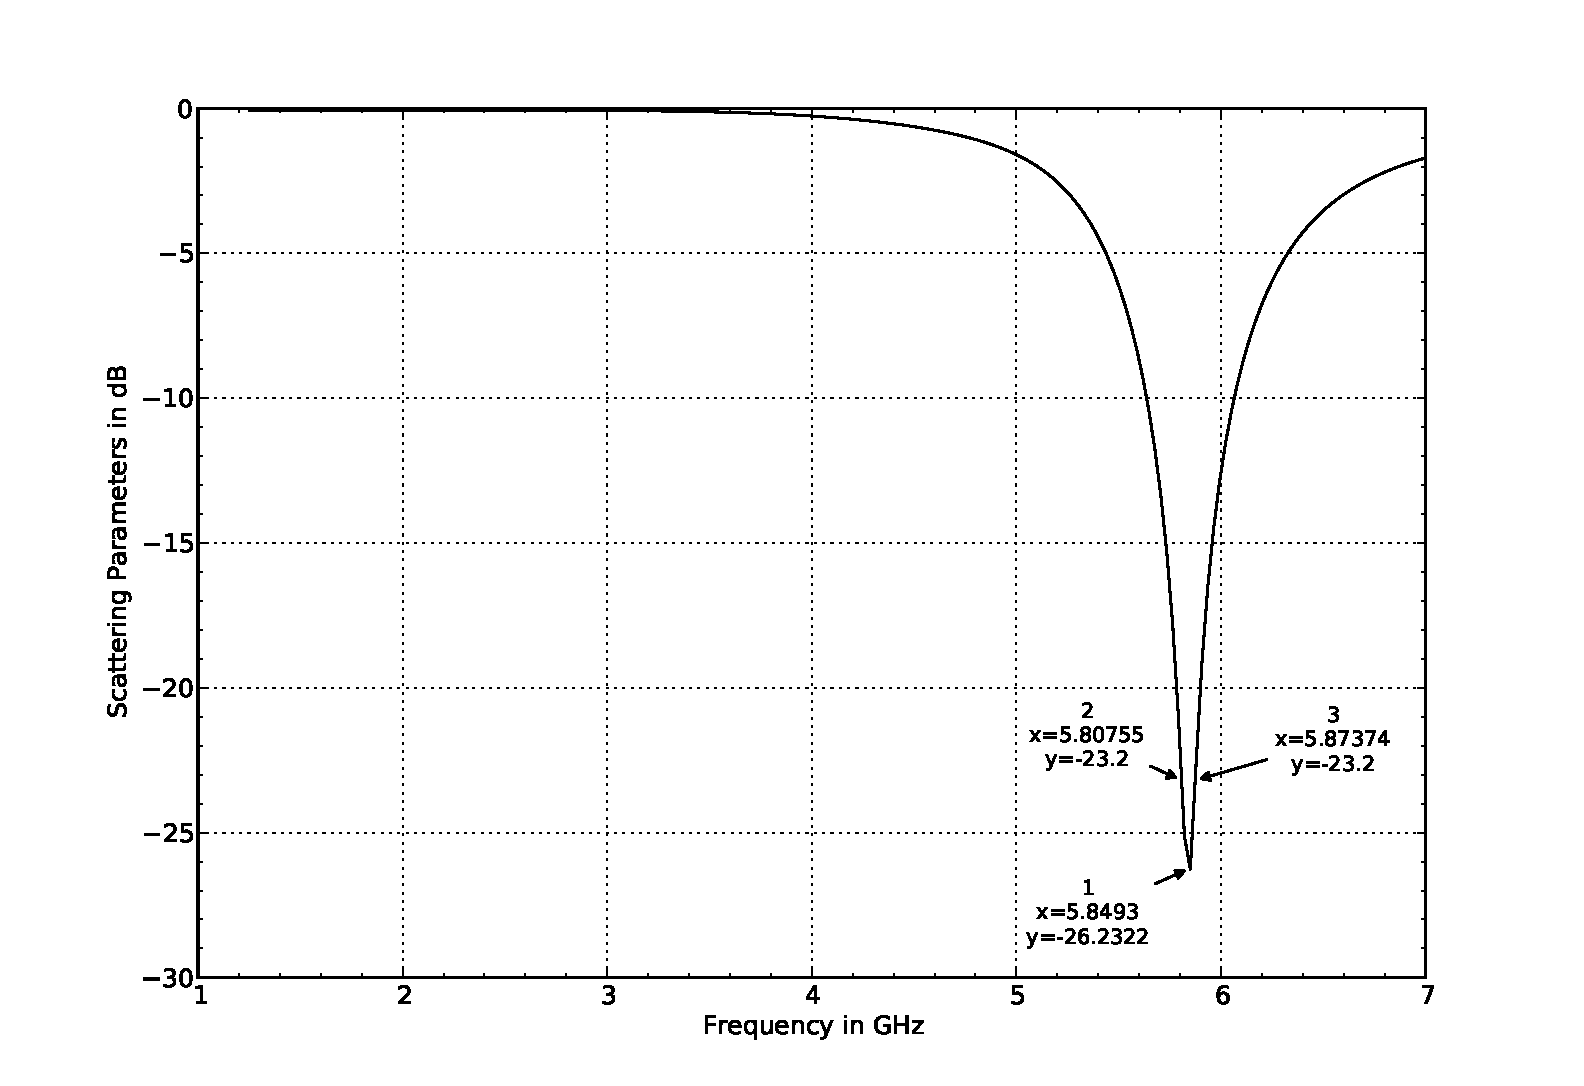
\includegraphics[width=\linewidth]{content/bilder/Evaluation/Loop/L2/ohneABS/S11_Loop_Lambda2_ohneABS.pdf}
%  \caption{\\$S_{11}$ Diagramm \\einer $\lambda/2$ Loop Antenne \\ im Freiraum}\label{fig:S11_Loop_Lambda2_freiraum_1}
%\endminipage%\hfill
%\minipage{0.4\textwidth}
%  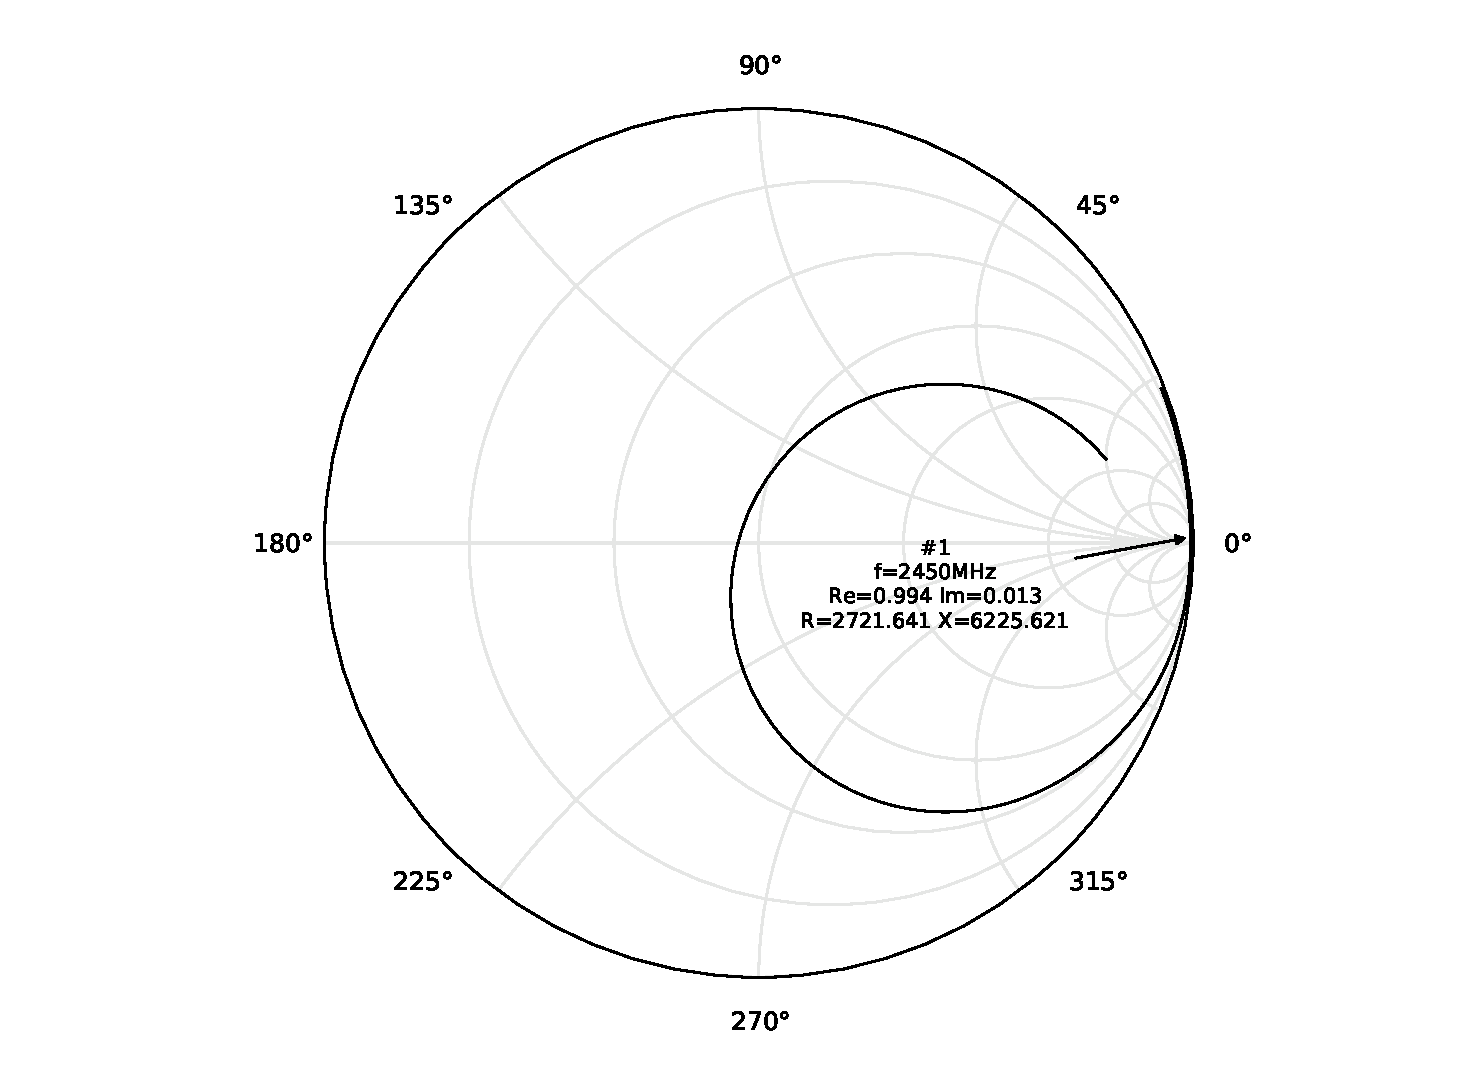
\includegraphics[width=\linewidth]{content/bilder/Evaluation/Loop/L2/ohneABS/Smith_Loop_Lambda2_ohneABS.pdf}
%  \caption{\\Smith Diagramm \\einer $\lambda/2$ Loop Antenne \\ im Freiraum}\label{fig:Smith_Loop_Lambda2_freiraum_2}
%\endminipage
%\end{center}
%\end{figure}
%%%%%%%%%%%%%%%%%%%%%%%
%\newpage
Die sehr tiefe Abstrahleffizienz ist auch aus der Abbildung \ref{fig:sim_Loop_freiraum_3D} zu entnehmen. Es ist kaum eine bevorzugte Abstrahlrichtung zu sehen. Die dunkelrote Farbe entspricht einem Richtfaktor von 1.19dBi, das enspricht beinahe einem isotropen Abstrahlverhalten.
%%%%%%%%%%%%%%%%%
%\begin{figure}[h]
%	\centering
%	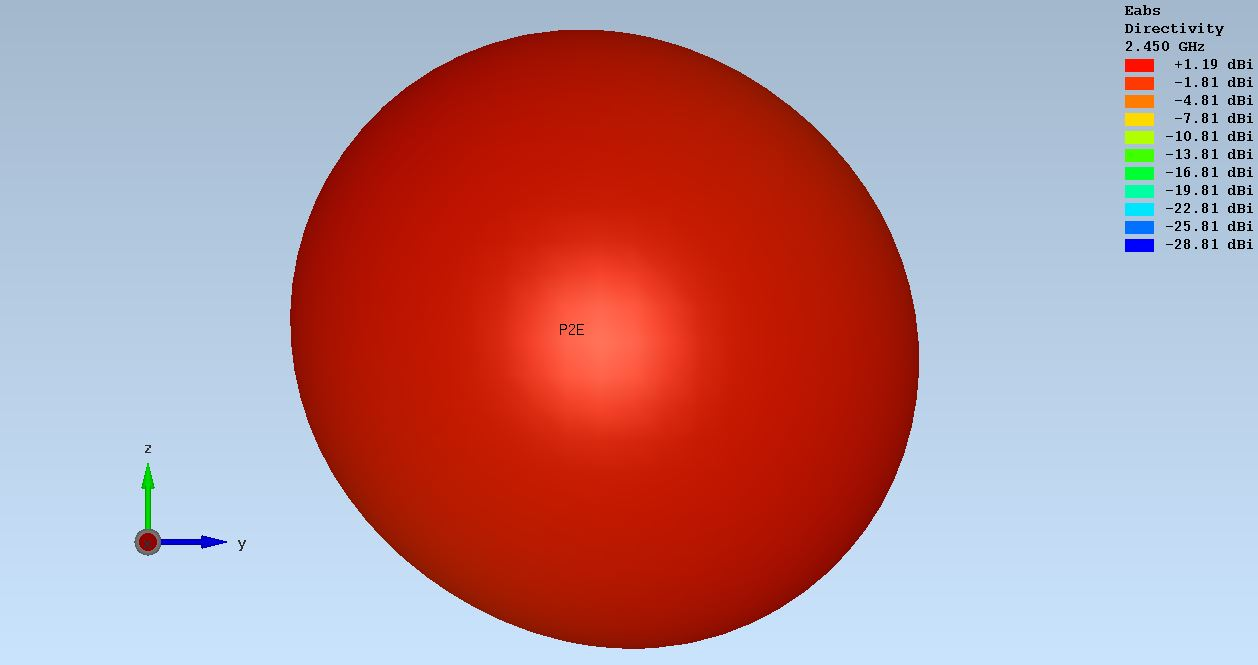
\includegraphics[width=8cm]{content/bilder/Evaluation/Loop/L2/ohneABS/EM_Far_Field_Loop_Lambda2_ohneABS.JPG}%
%	\caption{Simulierte 3D Abstrahlcharakteristik eines $\lambda/2$ Loops}
%	\label{fig:sim_Loop_freiraum_3D}
%\end{figure}
%%%%%%%%%%%%%%%%%%%%%%%
%%%%%%%%%%%%%%%%%%%%%%%%%%%%%%%%%%%%%%%%%%%%%%%%%%%%%%
\newpage
\textbf{$\lambda/2$ Loop Antenne mit ABS Stück im Nahfeld}\\
Die Simulationen der Dipolantennen haben eine erhebliche Wirkung des ABS Kunststoffs auf die Resonanzfrequenz gezeigt. Da die Loopantenne in ihrem Nahfeld ein starkes Magnetfeld zeigt und der elektrisch nicht leitende ABS Kunststoff  nicht magnetisch ist, sollte dieser keine grosse Wirkung auf die Resonanzfrequenz zeigen.\\ Diese Erwartungshaltung kann mit der folgenden Simulation überprüft werden.\\
 
Die Abbildung \ref{fig:S11_Lambda2_Loop_1ABS_3} zeigt das $S_{11}$ Diagramm derselben Loopantenne wie in Abbildung \ref{fig:Smith_Loop_Lambda2_freiraum_2}. Jedoch wird wie bei den Simulationen der Dipolantenne ein ABS Kunststoffstück direkt an die Antenne gelegt. Das ABS Stück hat die Masse 100 x 30 x 2 mm (L x B x H). Die Abmessungen der Antennenstruktur und die Simulationseigenschaften bleiben  dieselben wie bei den Dipolsimulationen und der Freiraum Simulation der Loop Antenne.\\

Die Abbildung \ref{fig:S11_Lambda2_Loop_1ABS_3} und \ref{fig:Smith_Lambda2_Loop_1ABS_4} zeigen jedoch eine Resonanzfrequenz, die um mehr als 1430MHz auf 4.41GHz gefallen ist. Die -10dB Bandbreite ist auf 350kHz gesunken. Weiter ist der $S_{11}$ maximal Wert auf -15.4dB gesunken.\\
Die Abbildung \ref{fig:Smith_Lambda2_Loop_1ABS_4} zeigt das Smith-Diagramm. Daraus ist ebenfalls ersichtlich, dass die Antenne für die Frequenz 2.45GHz nicht mehr einen Unterbruch darstellt. Die Abstrahleffizienz ist immer noch unter $3\%$. Das ist auf die Antennenimpedanz $Z_{ant}$ von (28-j433)Ohm zurückzuführen.
%%%%%%%%%%%%%%%%%%%
%Simulation S11 Loop

%%%%%%%%%%%%%%%%%%

%\begin{figure}[!h]
%\begin{center}
%\minipage{0.4\textwidth}
%  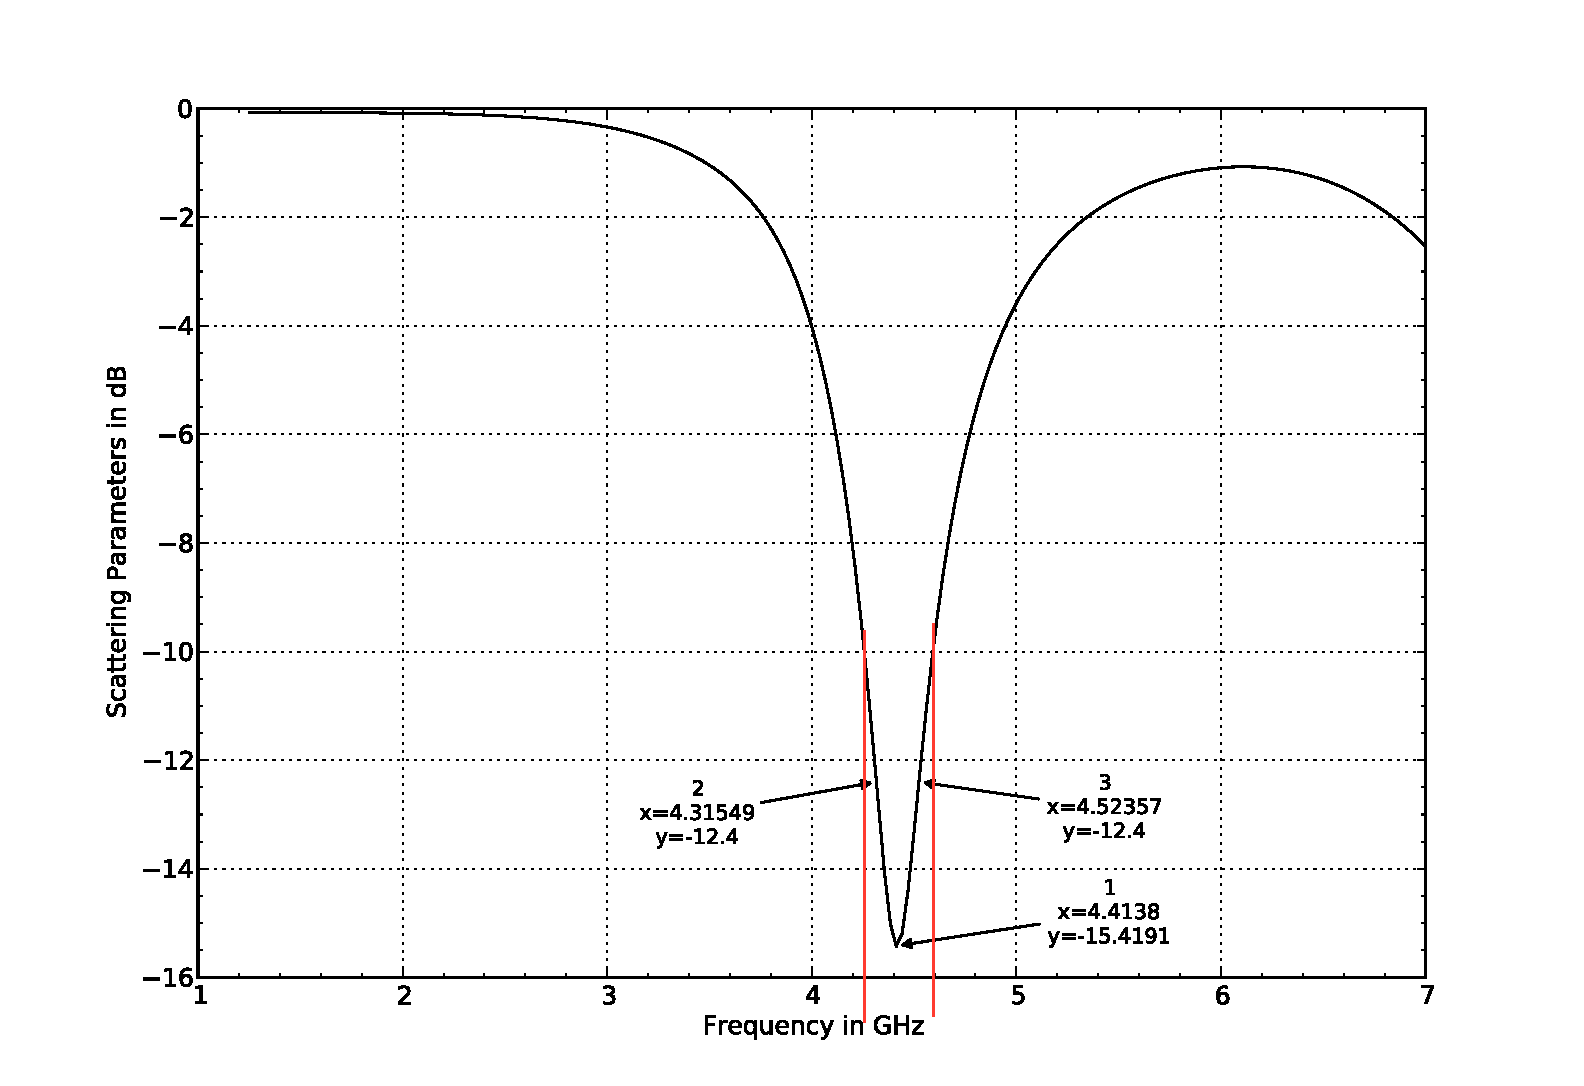
\includegraphics[width=\linewidth]{content/bilder/Evaluation/Loop/L2/1ABS/S11_Loop_Lambda2_mitABS.pdf}
%  \caption{\\$S_{11}$ Diagramm \\einer $\lambda/2$ Loop Antenne \\mit einem ABS Stück im Nahfeld}\label{fig:S11_Lambda2_Loop_1ABS_3}
%\endminipage%\hfill
%\minipage{0.4\textwidth}
%  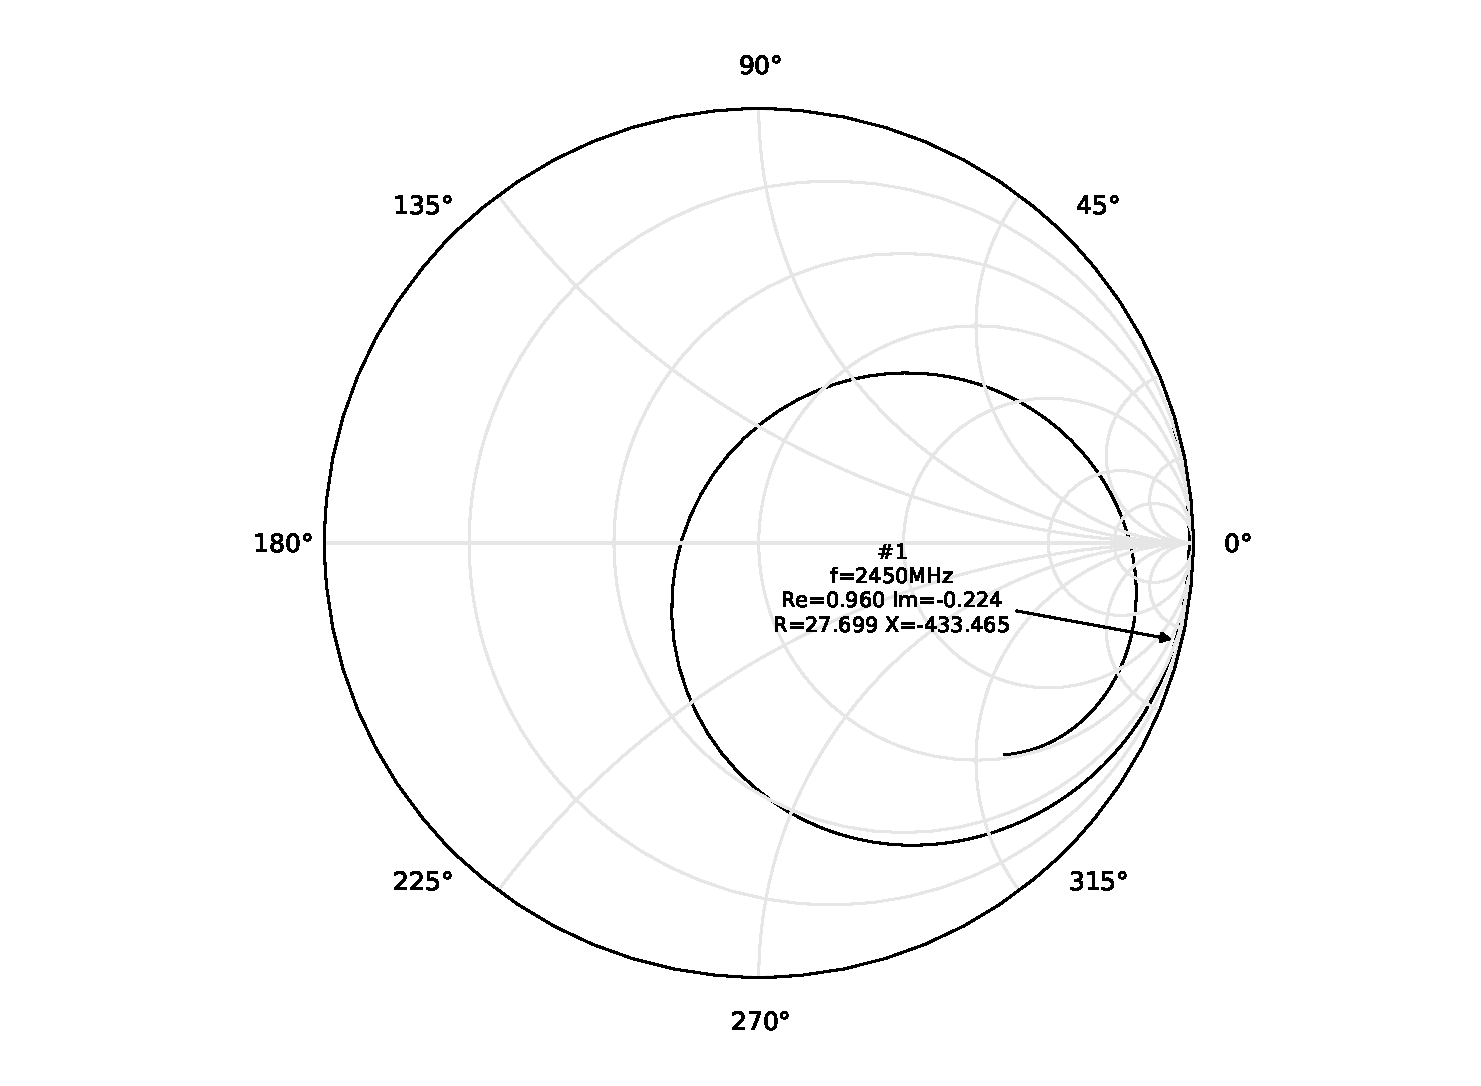
\includegraphics[width=\linewidth]{content/bilder/Evaluation/Loop/L2/1ABS/Smith_Loop_Lambda2_mitABS.pdf}
%  \caption{\\Smith Diagramm \\einer $\lambda/2$ Loop Antenne \\ mit einem ABS Stück im Nahfeld}\label{fig:Smith_Lambda2_Loop_1ABS_4}
%\endminipage
%\end{center}
%\end{figure}
%%%%%%%%%%%%%%%%%%%%%%%%
%\newpage
Das simulierte 3D Richtdiagramm des $\lambda/2$ langen und flachen Dipols zeigt weiterhin keine eindeutig bevorzugte Richtwirkung. Der D Wert liegt bei 1.54dBi, das ist etwa derselebe Wert einer $\lambda/2$ Dipolantenne. 
%%%%%%%%%%%%%%%%%%%%%%%
%\begin{figure}[h]
%	\centering
%	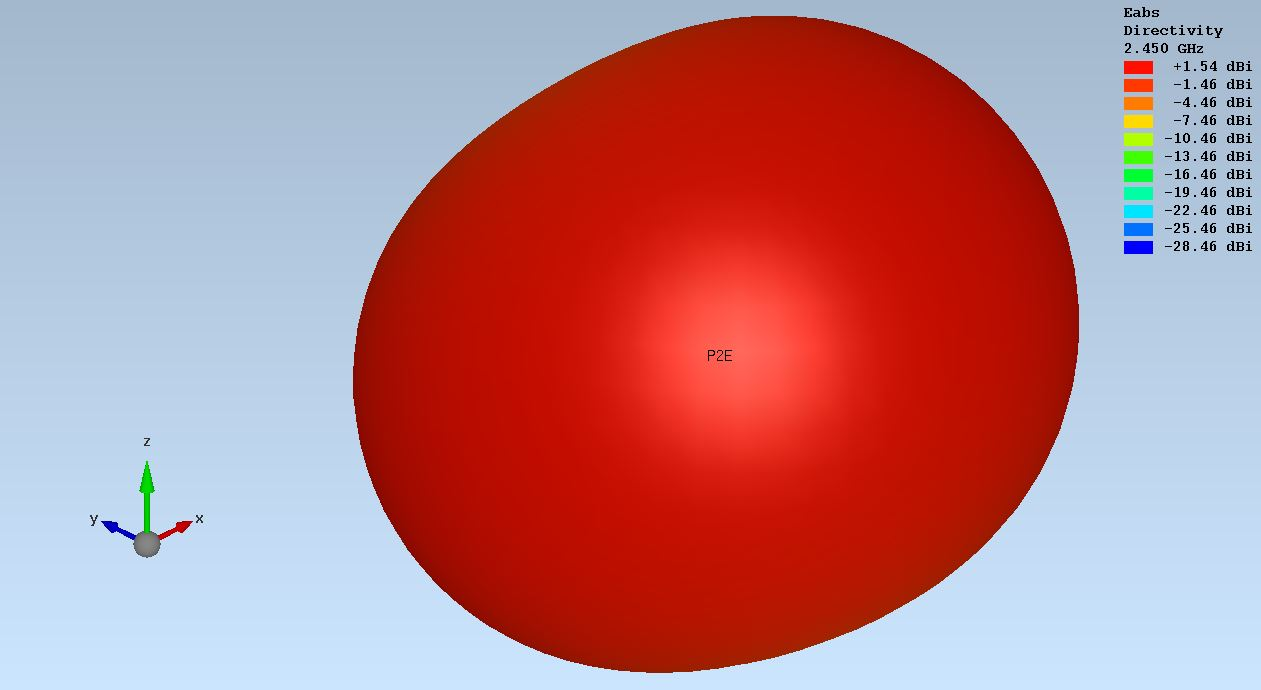
\includegraphics[width=8cm]{content/bilder/Evaluation/Loop/L2/1ABS/EM_Far_Field_Loop_Lambda2_mitABS.JPG}%
%	\caption{Simulierte 3D Abstrahlcharakteristik eines $\lambda/2$ Loops mit einem ABS Stück im Nahfeld}
%	\label{fig:sim_Loop_freiraum_3D_1ABS}
%\end{figure}
%%%%%%%%%%%%%%%%%%%%%%%
%%%%%%%%%%%%%%%%%%%%%%%%%%%%%%%%%%%%%%%%%%%%%%%%%%%%%%

\textbf{$\lambda/2$ Loop Antenne mit zwei ABS Stücken im Nahfeld}\\
Die Simulationen der Loopantenne mit ABS Kunststoff im Nahfeld  zeigt, dass der Kunststoff  Auswirkungen auf die Resonanzfrequenz in ähnlicher Art und Weise wie bei einer Dipolantenne zeigt.\\

Die Loop Antenne wird nun zwischen zwei gleich grossen ABS Kunststoffstücken eingeklemmt. Die Antennenanordnung und Ausrichtung der Antenne bleibt dieselbe. \\
Die Erwartung ist, dass auch bei dieser Simulation ein Detunig stattfindet.\\ 

Die Abbildung \ref{fig:S11_Lambda2_Loop_2ABS_5} zeigt, dass die Resonanzfrequenz weiter sinkt. Sie liegt neu bei 4.3GHz. Die -10dB Bandbreite beträgt 270 MHz. Der $S_{11}$ Wert zeigt bei 4.3GHz -13.2dB.\\
Das Smith Diagramm in Abbildung \ref{fig:Smith_Lambda2_Loop_2ABS_6} zeigt einen Antennenwiderstand von $24\Omega$ und einen kapazitiven Anteil von $-j379\Omega$\\
%\begin{figure}[!ht]
%	\begin{center}
%	\minipage{0.4\textwidth}
% 	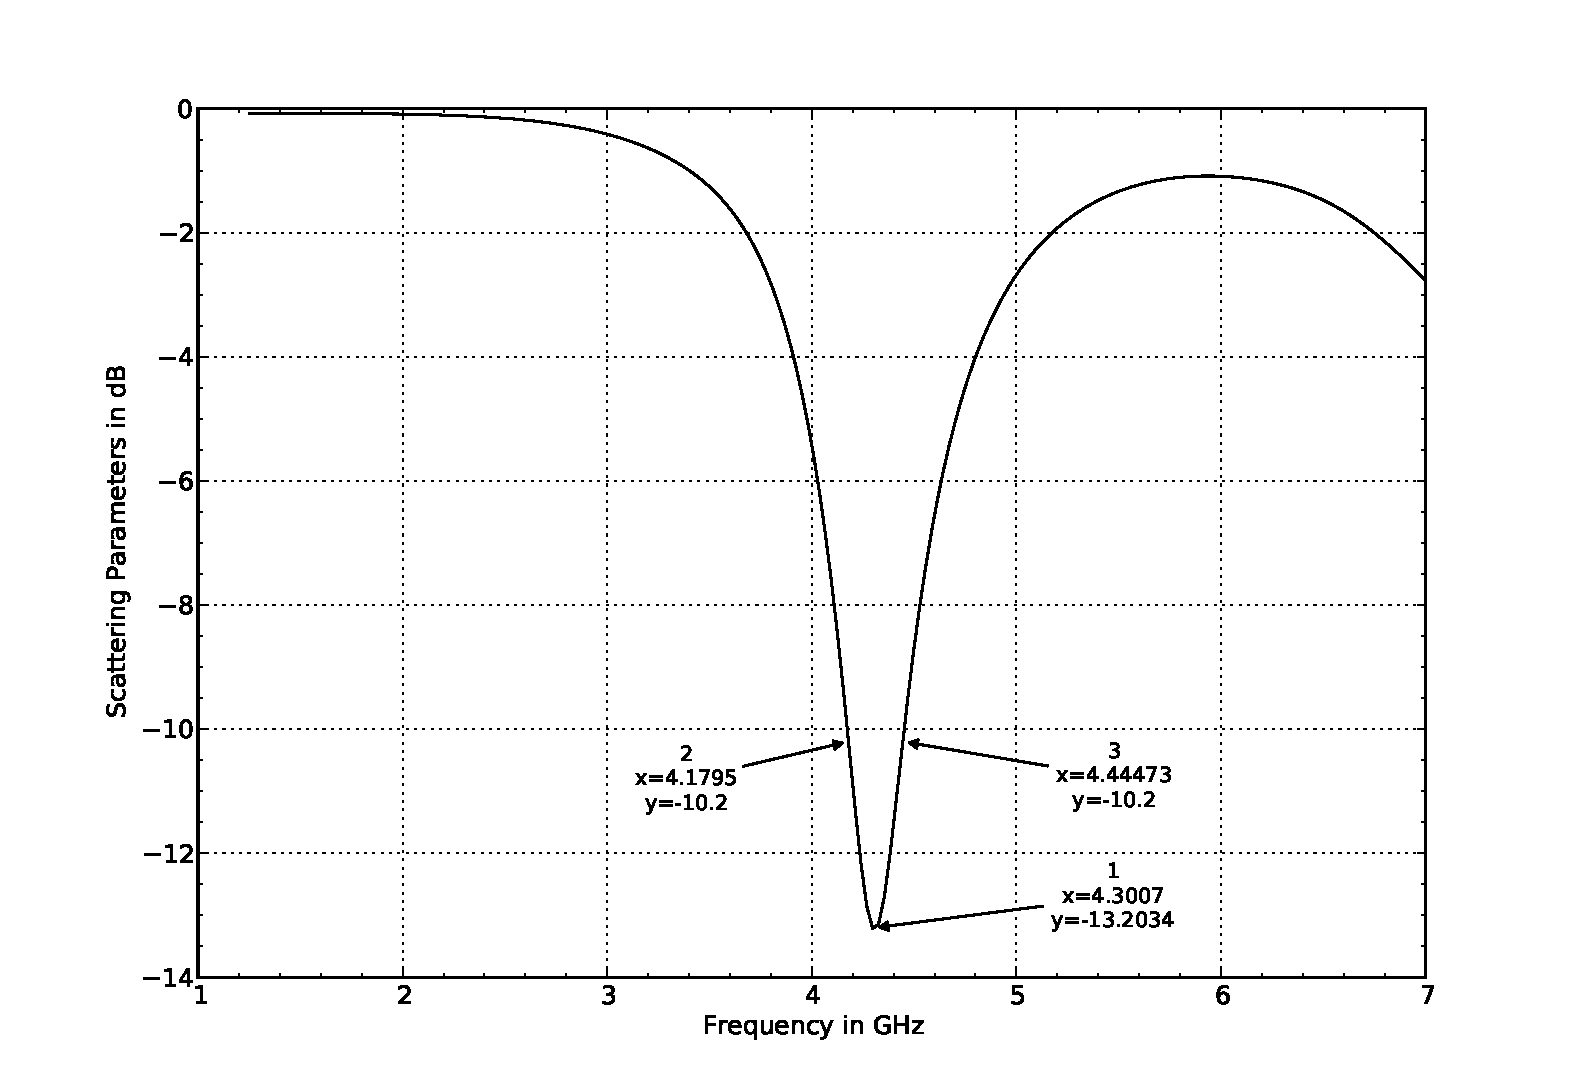
\includegraphics[width=\linewidth]{content/bilder/Evaluation/Loop/L2/2ABS/S11_Loop_Lambda2_mit2ABS.pdf}
%  	\caption{\\$S_{11}$ Diagramm \\einer $\lambda/2$ Loop Antenne \\mit zwei ABS Stücken im Nahfeld}				\label{fig:S11_Lambda2_Loop_2ABS_5}
%\endminipage%\hfill
%	\minipage{0.4\textwidth}
% 	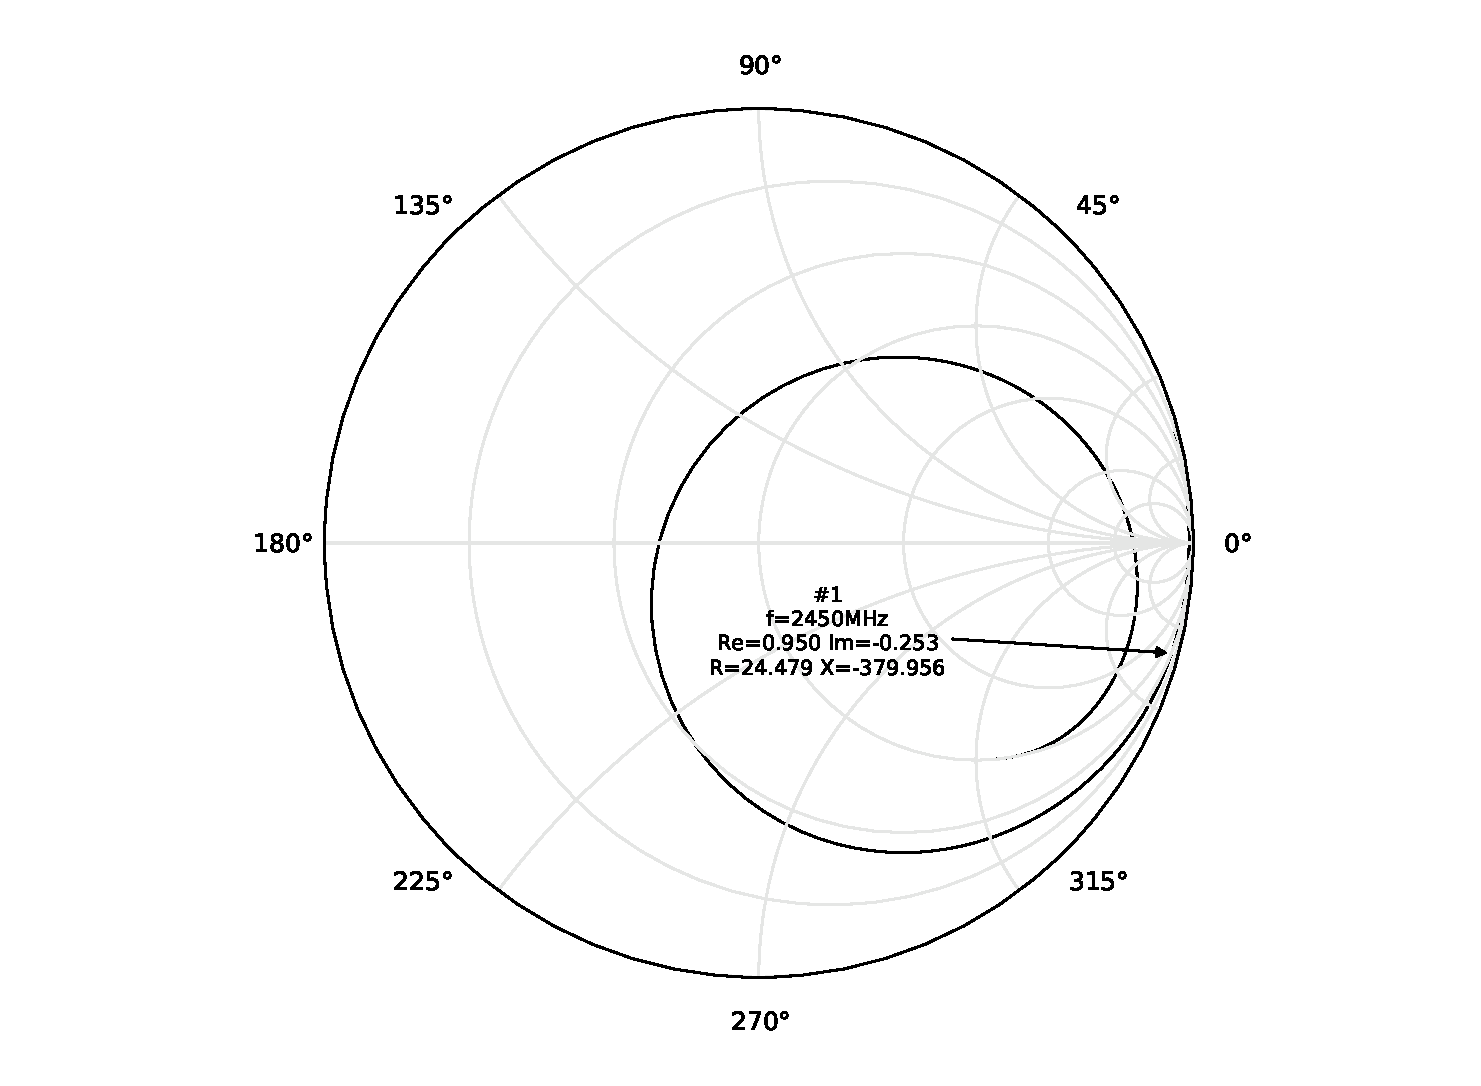
\includegraphics[width=\linewidth]{content/bilder/Evaluation/Loop/L2/2ABS/Smith_Loop_Lambda2_mit2ABS.pdf}
%  	\caption{\\Smith-Diagramm \\einer $\lambda/2$ Loop Antenne \\ mit zwei ABS Stücken im Nahfeld}		\label{fig:Smith_Lambda2_Loop_2ABS_6}
%	\endminipage
%	\end{center}
%\end{figure}
%%%%%%%%%%%%%%%%%%%%%%%
%\newpage
Die Simulationen der Loopantenne mit ABS Kunststoff im Nahfeld  zeigt, dass der Kunststoff  Auswirkungen auf die Resonanzfrequenz in ähnlicher Weise wie bei einer Dipolantenne zeigt.\\
Die Abstrahleffizienz ist knapp über $3\%$. Die erhebliche Fehlanpassung macht sich deutlich bemerkbar. Die Abstrahlrichtung mit der stärksten Ausprägung zeigt nur 1.59dBi. Das ist in der Abbildung \ref{fig:sim_Loop_freiraum_3D_2ABS} gezeigt.
%%%%%%%%%%%%%%%%
%\begin{figure}[h]
%	\centering
%	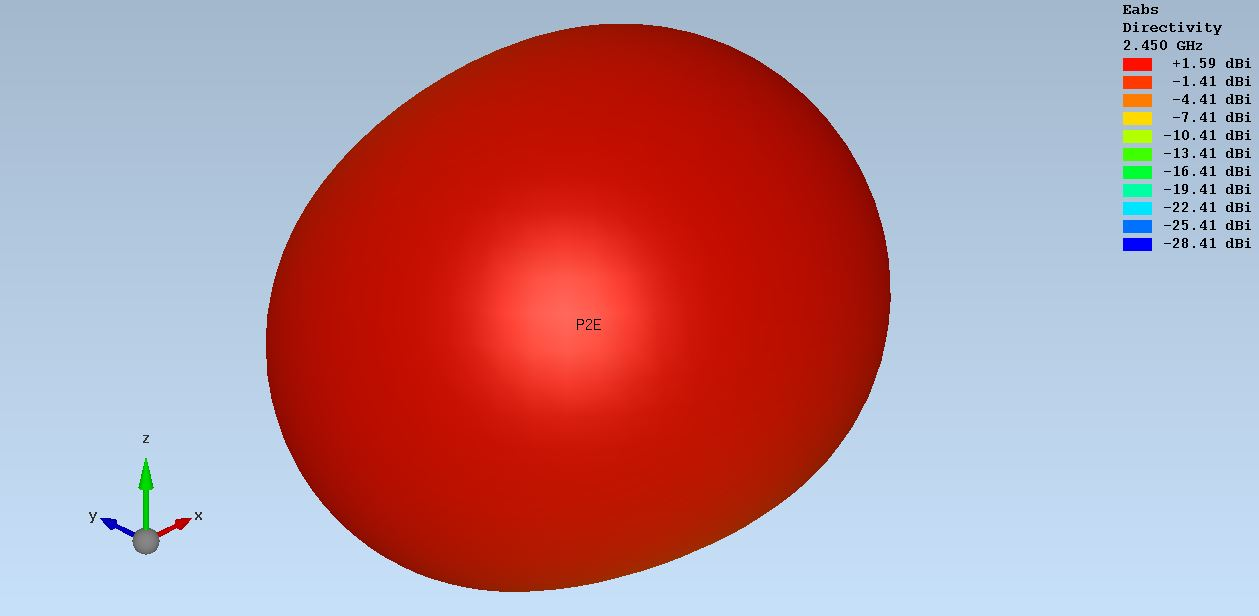
\includegraphics[width=8cm]{content/bilder/Evaluation/Loop/L2/2ABS/EM_Far_Field_Loop_Lambda2_mit2ABS.JPG}%
%	\caption{Simulierte 3D Abstrahlcharakteristik eines $\lambda/2$ Loops mit einem ABS Stück im Nahfeld}
%	\label{fig:sim_Loop_freiraum_3D_2ABS}
%\end{figure}
%%%%%%%%%%%%%%%%%%%%%%%
%%%%%%%%%%%%%%%%%%%%%%%%%%%%%%%%%%%%%%%%%%%%%%%%%%%%%%
%\clearpage
%%%%%%%%%%%%%%%%%%
\begin{figure}[!ht]
	\centering
	\begingroup
	\inputencoding{latin1}
	% This file was created by matlab2tikz.
%
%The latest updates can be retrieved from
%  http://www.mathworks.com/matlabcentral/fileexchange/22022-matlab2tikz-matlab2tikz
%where you can also make suggestions and rate matlab2tikz.
%
\begin{tikzpicture}

\begin{axis}[%
width=6in,
height=4.5in,
at={(0.758in,0.481in)},
scale only axis,
separate axis lines,
every outer x axis line/.append style={black},
every x tick label/.append style={font=\color{black}},
xmin=1,
xmax=7,
xlabel={Frequenz in [GHz]},
xmajorgrids,
every outer y axis line/.append style={black},
every y tick label/.append style={font=\color{black}},
ymin=-30,
ymax=0,
ylabel={Amplitude in [dB]},
ymajorgrids,
axis background/.style={fill=white},
title={$\text{Simulation des  $$S}_{\text{11}}\text{$$ einer Loop Antnne im Freiraum, mit einem und zwei ABS-St�cken}$},
legend style={at={(0.03,0.03)},anchor=south west,legend cell align=left,align=left,draw=black}
]
\addplot [color=red,very thick,solid]
  table[row sep=crcr]{%
1.25	-0.0654653\\
1.27875	-0.065151\\
1.3075	-0.0648209\\
1.33625	-0.0644764\\
1.365	-0.0641187\\
1.39375	-0.063749\\
1.4225	-0.0633686\\
1.45125	-0.0629787\\
1.48	-0.0625805\\
1.50875	-0.0621748\\
1.5375	-0.0617627\\
1.56625	-0.0613451\\
1.595	-0.0609229\\
1.62375	-0.0604971\\
1.6525	-0.0600686\\
1.68125	-0.0596384\\
1.71	-0.0592073\\
1.73875	-0.058776\\
1.7675	-0.0583456\\
1.79625	-0.057917\\
1.825	-0.0574911\\
1.85375	-0.057069\\
1.8825	-0.0566517\\
1.91125	-0.05624\\
1.94	-0.055835\\
1.96875	-0.0554378\\
1.9975	-0.0550496\\
2.02625	-0.0546716\\
2.055	-0.0543049\\
2.08375	-0.0539509\\
2.1125	-0.0536108\\
2.14125	-0.053286\\
2.17	-0.052978\\
2.19875	-0.0526882\\
2.2275	-0.0524183\\
2.25625	-0.0521699\\
2.285	-0.0519448\\
2.31375	-0.051745\\
2.3425	-0.0515722\\
2.37125	-0.0514284\\
2.4	-0.0513159\\
2.42875	-0.0512366\\
2.4575	-0.051193\\
2.48625	-0.0511876\\
2.515	-0.0512229\\
2.54375	-0.0513016\\
2.5725	-0.0514267\\
2.60125	-0.0516011\\
2.63	-0.0518279\\
2.65875	-0.0521105\\
2.6875	-0.0524524\\
2.71625	-0.0528571\\
2.745	-0.0533287\\
2.77375	-0.0538711\\
2.8025	-0.0544888\\
2.83125	-0.0551862\\
2.86	-0.055968\\
2.88875	-0.0568393\\
2.9175	-0.0578054\\
2.94625	-0.0588719\\
2.975	-0.0600447\\
3.00375	-0.06133\\
3.0325	-0.0627342\\
3.06125	-0.0642643\\
3.09	-0.0659274\\
3.11875	-0.0677313\\
3.1475	-0.069684\\
3.17625	-0.0717941\\
3.205	-0.0740707\\
3.23375	-0.0765229\\
3.2625	-0.0791608\\
3.29125	-0.0819948\\
3.32	-0.0850359\\
3.34875	-0.0882959\\
3.3775	-0.0917869\\
3.40625	-0.0955216\\
3.435	-0.0995135\\
3.46375	-0.103777\\
3.4925	-0.108326\\
3.52125	-0.113178\\
3.55	-0.118347\\
3.57875	-0.123852\\
3.6075	-0.129711\\
3.63625	-0.135941\\
3.665	-0.142562\\
3.69375	-0.149595\\
3.7225	-0.157061\\
3.75125	-0.164982\\
3.78	-0.173381\\
3.80875	-0.18228\\
3.8375	-0.191706\\
3.86625	-0.201682\\
3.895	-0.212235\\
3.92375	-0.223392\\
3.9525	-0.235181\\
3.98125	-0.247628\\
4.01	-0.260763\\
4.03875	-0.274617\\
4.0675	-0.289219\\
4.09625	-0.3046\\
4.125	-0.320793\\
4.15375	-0.337829\\
4.1825	-0.355743\\
4.21125	-0.374571\\
4.24	-0.394349\\
4.26875	-0.415117\\
4.2975	-0.436915\\
4.32625	-0.459787\\
4.355	-0.483783\\
4.38375	-0.508955\\
4.4125	-0.535362\\
4.44125	-0.563071\\
4.47	-0.592156\\
4.49875	-0.622701\\
4.5275	-0.654803\\
4.55625	-0.688572\\
4.585	-0.724136\\
4.61375	-0.761639\\
4.6425	-0.80125\\
4.67125	-0.843159\\
4.7	-0.887585\\
4.72875	-0.934776\\
4.7575	-0.985017\\
4.78625	-1.03863\\
4.815	-1.09598\\
4.84375	-1.15748\\
4.8725	-1.2236\\
4.90125	-1.29486\\
4.93	-1.37186\\
4.95875	-1.45525\\
4.9875	-1.5458\\
5.01625	-1.64433\\
5.045	-1.7518\\
5.07375	-1.86926\\
5.1025	-1.99793\\
5.13125	-2.13916\\
5.16	-2.29446\\
5.18875	-2.46556\\
5.2175	-2.65443\\
5.24625	-2.86328\\
5.275	-3.09464\\
5.30375	-3.35139\\
5.3325	-3.63684\\
5.36125	-3.95479\\
5.39	-4.30964\\
5.41875	-4.70652\\
5.4475	-5.15145\\
5.47625	-5.6516\\
5.505	-6.21558\\
5.53375	-6.85395\\
5.5625	-7.57989\\
5.59125	-8.41027\\
5.62	-9.36735\\
5.64875	-10.4815\\
5.6775	-11.796\\
5.70625	-13.3755\\
5.735	-15.3218\\
5.76375	-17.8029\\
5.7925	-21.0803\\
5.82125	-25.1285\\
5.85	-26.2598\\
5.87875	-22.5541\\
5.9075	-19.0602\\
5.93625	-16.4463\\
5.965	-14.4415\\
5.99375	-12.8455\\
6.0225	-11.5373\\
6.05125	-10.4414\\
6.08	-9.50797\\
6.10875	-8.70272\\
6.1375	-8.00095\\
6.16625	-7.38427\\
6.195	-6.83863\\
6.22375	-6.35301\\
6.2525	-5.91861\\
6.28125	-5.52831\\
6.31	-5.17624\\
6.33875	-4.85752\\
6.3675	-4.56805\\
6.39625	-4.30435\\
6.425	-4.06347\\
6.45375	-3.84286\\
6.4825	-3.64031\\
6.51125	-3.45393\\
6.54	-3.28206\\
6.56875	-3.12324\\
6.5975	-2.9762\\
6.62625	-2.83981\\
6.655	-2.71309\\
6.68375	-2.59514\\
6.7125	-2.48519\\
6.74125	-2.38255\\
6.77	-2.28659\\
6.79875	-2.19675\\
6.8275	-2.11254\\
6.85625	-2.03351\\
6.885	-1.95925\\
6.91375	-1.8894\\
6.9425	-1.82363\\
6.97125	-1.76165\\
7	-1.70318\\
};
\addlegendentry{$\text{S}_{\text{11}}\text{ Freiraum}$};

\addplot [color=blue,very thick,solid]
  table[row sep=crcr]{%
1.25	-0.0742623\\
1.27875	-0.0743003\\
1.3075	-0.074338\\
1.33625	-0.074378\\
1.365	-0.0744227\\
1.39375	-0.0744748\\
1.4225	-0.074537\\
1.45125	-0.0746122\\
1.48	-0.0747032\\
1.50875	-0.074813\\
1.5375	-0.074945\\
1.56625	-0.0751024\\
1.595	-0.075289\\
1.62375	-0.0755086\\
1.6525	-0.0757651\\
1.68125	-0.0760628\\
1.71	-0.0764064\\
1.73875	-0.0768005\\
1.7675	-0.0772505\\
1.79625	-0.0777618\\
1.825	-0.0783403\\
1.85375	-0.0789924\\
1.8825	-0.0797245\\
1.91125	-0.0805441\\
1.94	-0.0814588\\
1.96875	-0.0824767\\
1.9975	-0.0836067\\
2.02625	-0.0848582\\
2.055	-0.0862413\\
2.08375	-0.0877667\\
2.1125	-0.0894459\\
2.14125	-0.0912913\\
2.17	-0.0933162\\
2.19875	-0.0955348\\
2.2275	-0.0979622\\
2.25625	-0.100615\\
2.285	-0.10351\\
2.31375	-0.106666\\
2.3425	-0.110103\\
2.37125	-0.113843\\
2.4	-0.117909\\
2.42875	-0.122324\\
2.4575	-0.127116\\
2.48625	-0.132313\\
2.515	-0.137945\\
2.54375	-0.144043\\
2.5725	-0.150643\\
2.60125	-0.157782\\
2.63	-0.165499\\
2.65875	-0.173836\\
2.6875	-0.182838\\
2.71625	-0.192554\\
2.745	-0.203035\\
2.77375	-0.214335\\
2.8025	-0.226512\\
2.83125	-0.23963\\
2.86	-0.253753\\
2.88875	-0.268952\\
2.9175	-0.285302\\
2.94625	-0.302882\\
2.975	-0.321774\\
3.00375	-0.34207\\
3.0325	-0.363862\\
3.06125	-0.38725\\
3.09	-0.412341\\
3.11875	-0.439246\\
3.1475	-0.468087\\
3.17625	-0.498989\\
3.205	-0.53209\\
3.23375	-0.567538\\
3.2625	-0.605492\\
3.29125	-0.646124\\
3.32	-0.689626\\
3.34875	-0.736209\\
3.3775	-0.786109\\
3.40625	-0.839592\\
3.435	-0.89696\\
3.46375	-0.958557\\
3.4925	-1.02478\\
3.52125	-1.09609\\
3.55	-1.17302\\
3.57875	-1.25618\\
3.6075	-1.3463\\
3.63625	-1.44419\\
3.665	-1.55084\\
3.69375	-1.66736\\
3.7225	-1.79503\\
3.75125	-1.93534\\
3.78	-2.09\\
3.80875	-2.26098\\
3.8375	-2.4505\\
3.86625	-2.66115\\
3.895	-2.89583\\
3.92375	-3.15789\\
3.9525	-3.4511\\
3.98125	-3.77978\\
4.01	-4.14883\\
4.03875	-4.5638\\
4.0675	-5.03102\\
4.09625	-5.55762\\
4.125	-6.15167\\
4.15375	-6.82216\\
4.1825	-7.57889\\
4.21125	-8.43199\\
4.24	-9.39049\\
4.26875	-10.4589\\
4.2975	-11.6289\\
4.32625	-12.8615\\
4.355	-14.0534\\
4.38375	-15.0001\\
4.4125	-15.4299\\
4.44125	-15.1923\\
4.47	-14.4132\\
4.49875	-13.361\\
4.5275	-12.248\\
4.55625	-11.1838\\
4.585	-10.2102\\
4.61375	-9.33644\\
4.6425	-8.5582\\
4.67125	-7.86635\\
4.7	-7.25083\\
4.72875	-6.70207\\
4.7575	-6.21151\\
4.78625	-5.77168\\
4.815	-5.37614\\
4.84375	-5.01936\\
4.8725	-4.6966\\
4.90125	-4.40379\\
4.93	-4.13743\\
4.95875	-3.89449\\
4.9875	-3.67238\\
5.01625	-3.46882\\
5.045	-3.28185\\
5.07375	-3.10976\\
5.1025	-2.95105\\
5.13125	-2.8044\\
5.16	-2.66866\\
5.18875	-2.54282\\
5.2175	-2.42598\\
5.24625	-2.31736\\
5.275	-2.21624\\
5.30375	-2.12202\\
5.3325	-2.03414\\
5.36125	-1.95211\\
5.39	-1.87549\\
5.41875	-1.80389\\
5.4475	-1.73697\\
5.47625	-1.67441\\
5.505	-1.61595\\
5.53375	-1.56133\\
5.5625	-1.51034\\
5.59125	-1.46278\\
5.62	-1.41848\\
5.64875	-1.37729\\
5.6775	-1.33907\\
5.70625	-1.30369\\
5.735	-1.27107\\
5.76375	-1.24111\\
5.7925	-1.21372\\
5.82125	-1.18886\\
5.85	-1.16645\\
5.87875	-1.14647\\
5.9075	-1.12887\\
5.93625	-1.11362\\
5.965	-1.10072\\
5.99375	-1.09015\\
6.0225	-1.08191\\
6.05125	-1.076\\
6.08	-1.07244\\
6.10875	-1.07124\\
6.1375	-1.07242\\
6.16625	-1.07602\\
6.195	-1.08206\\
6.22375	-1.09058\\
6.2525	-1.10164\\
6.28125	-1.11527\\
6.31	-1.13153\\
6.33875	-1.15048\\
6.3675	-1.17218\\
6.39625	-1.1967\\
6.425	-1.22411\\
6.45375	-1.2545\\
6.4825	-1.28793\\
6.51125	-1.32451\\
6.54	-1.36432\\
6.56875	-1.40747\\
6.5975	-1.45406\\
6.62625	-1.5042\\
6.655	-1.55801\\
6.68375	-1.6156\\
6.7125	-1.67711\\
6.74125	-1.74265\\
6.77	-1.81236\\
6.79875	-1.88635\\
6.8275	-1.96475\\
6.85625	-2.04769\\
6.885	-2.13525\\
6.91375	-2.22755\\
6.9425	-2.32465\\
6.97125	-2.42662\\
7	-2.53347\\
};
\addlegendentry{$\text{S}_{\text{11}}\text{ mit 1 ABS}$};

\addplot [color=green,very thick,solid]
  table[row sep=crcr]{%
1.25	-0.0745723\\
1.27875	-0.0746474\\
1.3075	-0.0747264\\
1.33625	-0.0748124\\
1.365	-0.0749084\\
1.39375	-0.0750178\\
1.4225	-0.0751437\\
1.45125	-0.0752898\\
1.48	-0.0754597\\
1.50875	-0.0756572\\
1.5375	-0.0758861\\
1.56625	-0.0761508\\
1.595	-0.0764558\\
1.62375	-0.076806\\
1.6525	-0.0772062\\
1.68125	-0.077662\\
1.71	-0.0781791\\
1.73875	-0.0787635\\
1.7675	-0.0794219\\
1.79625	-0.0801612\\
1.825	-0.0809889\\
1.85375	-0.081913\\
1.8825	-0.0829421\\
1.91125	-0.0840853\\
1.94	-0.0853527\\
1.96875	-0.0867545\\
1.9975	-0.0883021\\
2.02625	-0.0900074\\
2.055	-0.0918833\\
2.08375	-0.0939436\\
2.1125	-0.0962029\\
2.14125	-0.0986771\\
2.17	-0.101383\\
2.19875	-0.104339\\
2.2275	-0.107564\\
2.25625	-0.111079\\
2.285	-0.114905\\
2.31375	-0.119066\\
2.3425	-0.123587\\
2.37125	-0.128494\\
2.4	-0.133816\\
2.42875	-0.139584\\
2.4575	-0.145828\\
2.48625	-0.152584\\
2.515	-0.159888\\
2.54375	-0.167777\\
2.5725	-0.176293\\
2.60125	-0.185478\\
2.63	-0.195379\\
2.65875	-0.206043\\
2.6875	-0.217523\\
2.71625	-0.229871\\
2.745	-0.243144\\
2.77375	-0.257403\\
2.8025	-0.27271\\
2.83125	-0.289133\\
2.86	-0.306741\\
2.88875	-0.325609\\
2.9175	-0.345816\\
2.94625	-0.367444\\
2.975	-0.390583\\
3.00375	-0.415327\\
3.0325	-0.441778\\
3.06125	-0.470044\\
3.09	-0.500243\\
3.11875	-0.532505\\
3.1475	-0.566973\\
3.17625	-0.603802\\
3.205	-0.643168\\
3.23375	-0.68527\\
3.2625	-0.730329\\
3.29125	-0.778599\\
3.32	-0.83037\\
3.34875	-0.885975\\
3.3775	-0.945796\\
3.40625	-1.01027\\
3.435	-1.07992\\
3.46375	-1.15532\\
3.4925	-1.23714\\
3.52125	-1.32618\\
3.55	-1.42333\\
3.57875	-1.52962\\
3.6075	-1.64624\\
3.63625	-1.77456\\
3.665	-1.91612\\
3.69375	-2.07271\\
3.7225	-2.24636\\
3.75125	-2.43938\\
3.78	-2.65439\\
3.80875	-2.89437\\
3.8375	-3.1627\\
3.86625	-3.46317\\
3.895	-3.80003\\
3.92375	-4.17804\\
3.9525	-4.60247\\
3.98125	-5.07905\\
4.01	-5.61394\\
4.03875	-6.21347\\
4.0675	-6.88372\\
4.09625	-7.62957\\
4.125	-8.45284\\
4.15375	-9.34872\\
4.1825	-10.2991\\
4.21125	-11.2616\\
4.24	-12.1549\\
4.26875	-12.8525\\
4.2975	-13.2107\\
4.32625	-13.145\\
4.355	-12.6927\\
4.38375	-11.9824\\
4.4125	-11.152\\
4.44125	-10.2992\\
4.47	-9.47877\\
4.49875	-8.71596\\
4.5275	-8.01917\\
4.55625	-7.38841\\
4.585	-6.81978\\
4.61375	-6.30787\\
4.6425	-5.84692\\
4.67125	-5.43138\\
4.7	-5.05616\\
4.72875	-4.71665\\
4.7575	-4.40882\\
4.78625	-4.12907\\
4.815	-3.87431\\
4.84375	-3.64178\\
4.8725	-3.42913\\
4.90125	-3.23425\\
4.93	-3.05535\\
4.95875	-2.89082\\
4.9875	-2.73928\\
5.01625	-2.5995\\
5.045	-2.4704\\
5.07375	-2.35103\\
5.1025	-2.24056\\
5.13125	-2.13824\\
5.16	-2.04341\\
5.18875	-1.95548\\
5.2175	-1.87394\\
5.24625	-1.79832\\
5.275	-1.72819\\
5.30375	-1.66318\\
5.3325	-1.60295\\
5.36125	-1.5472\\
5.39	-1.49565\\
5.41875	-1.44806\\
5.4475	-1.40419\\
5.47625	-1.36385\\
5.505	-1.32685\\
5.53375	-1.29303\\
5.5625	-1.26222\\
5.59125	-1.23429\\
5.62	-1.20911\\
5.64875	-1.18656\\
5.6775	-1.16654\\
5.70625	-1.14894\\
5.735	-1.13367\\
5.76375	-1.12064\\
5.7925	-1.10978\\
5.82125	-1.10101\\
5.85	-1.09428\\
5.87875	-1.08951\\
5.9075	-1.08666\\
5.93625	-1.08568\\
5.965	-1.08655\\
5.99375	-1.08923\\
6.0225	-1.09372\\
6.05125	-1.10001\\
6.08	-1.10811\\
6.10875	-1.11805\\
6.1375	-1.12986\\
6.16625	-1.14359\\
6.195	-1.1593\\
6.22375	-1.17707\\
6.2525	-1.19699\\
6.28125	-1.21916\\
6.31	-1.24369\\
6.33875	-1.27072\\
6.3675	-1.30036\\
6.39625	-1.33276\\
6.425	-1.36807\\
6.45375	-1.40641\\
6.4825	-1.44794\\
6.51125	-1.49278\\
6.54	-1.54105\\
6.56875	-1.59286\\
6.5975	-1.64828\\
6.62625	-1.70736\\
6.655	-1.77012\\
6.68375	-1.83655\\
6.7125	-1.90658\\
6.74125	-1.98013\\
6.77	-2.05707\\
6.79875	-2.13724\\
6.8275	-2.22047\\
6.85625	-2.30657\\
6.885	-2.39536\\
6.91375	-2.48666\\
6.9425	-2.58034\\
6.97125	-2.67628\\
7	-2.77443\\
};
\addlegendentry{$\text{S}_{\text{11}}\text{ mit 2 ABS}$};

\end{axis}
\end{tikzpicture}%
	\endgroup
	\caption{Vergleich des $S_{11}$ Werts einer Loop Antenne}
	\label{S11_Loop_Vergleich_Simulation}
\end{figure}
%%%%%%%%%%%%%%%%%%%%%%%%%%%%%%%%%%%%%%%%%%%%%%%%%%%%%%%
\begin{figure}[!ht]
	\centering
	\begingroup
	\inputencoding{latin1}
	% This file was created by matlab2tikz.
%
%The latest updates can be retrieved from
%  http://www.mathworks.com/matlabcentral/fileexchange/22022-matlab2tikz-matlab2tikz
%where you can also make suggestions and rate matlab2tikz.
%
\definecolor{mycolor1}{rgb}{1.00000,1.00000,0.00000}%
\definecolor{mycolor2}{rgb}{1.00000,0.00000,1.00000}%
%
\begin{tikzpicture}

\begin{axis}[%
width=6in,
height=4.5in,
at={(1.327in,0.793in)},
scale only axis,
separate axis lines,
every outer x axis line/.append style={black},
every x tick label/.append style={font=\color{black}},
xmin=1.94342105263158,
xmax=3.04868421052632,
xlabel={Frequenz in [GHz]},
xmajorgrids,
every outer y axis line/.append style={black},
every y tick label/.append style={font=\color{black}},
ymin=-8.6968085106383,
ymax=17.2074468085106,
ylabel={Impedanz [Ohm]},
ymajorgrids,
axis background/.style={fill=white},
title={Impedanz der Loop Antenne im Freiraum, mit einem und zwei ABS St�cken},
legend style={legend cell align=left,align=left,draw=black}
]
\addplot [color=red,solid]
  table[row sep=crcr]{%
1.25	0.00568428\\
1.27875	0.00607318\\
1.3075	0.00648872\\
1.33625	0.00693341\\
1.365	0.00741008\\
1.39375	0.00792195\\
1.4225	0.00847266\\
1.45125	0.00906638\\
1.48	0.00970787\\
1.50875	0.0104026\\
1.5375	0.0111567\\
1.56625	0.0119776\\
1.595	0.0128735\\
1.62375	0.0138543\\
1.6525	0.0149314\\
1.68125	0.0161184\\
1.71	0.0174311\\
1.73875	0.0188886\\
1.7675	0.0205136\\
1.79625	0.0223335\\
1.825	0.0243817\\
1.85375	0.0266989\\
1.8825	0.0293356\\
1.91125	0.0323543\\
1.94	0.035834\\
1.96875	0.0398749\\
1.9975	0.0446063\\
2.02625	0.0501967\\
2.055	0.0568693\\
2.08375	0.0649243\\
2.1125	0.0747737\\
2.14125	0.0869941\\
2.17	0.102413\\
2.19875	0.122252\\
2.2275	0.148371\\
2.25625	0.183715\\
2.285	0.233169\\
2.31375	0.3053\\
2.3425	0.416225\\
2.37125	0.59911\\
2.4	0.93077\\
2.42875	1.61997\\
2.4575	3.36959\\
2.48625	8.97118\\
2.515	16.7337\\
2.54375	7.15955\\
2.5725	2.86676\\
2.60125	1.46122\\
2.63	0.874964\\
2.65875	0.581222\\
2.6875	0.414484\\
2.71625	0.311128\\
2.745	0.242772\\
2.77375	0.195269\\
2.8025	0.160949\\
2.83125	0.135366\\
2.86	0.1158\\
2.88875	0.100512\\
2.9175	0.0883501\\
2.94625	0.0785256\\
2.975	0.0704843\\
3.00375	0.063827\\
3.0325	0.058261\\
3.06125	0.053567\\
3.09	0.0495787\\
3.11875	0.0461677\\
3.1475	0.043234\\
3.17625	0.0406983\\
3.205	0.0384974\\
3.23375	0.0365803\\
3.2625	0.0349054\\
3.29125	0.0334386\\
3.32	0.0321519\\
3.34875	0.0310217\\
3.3775	0.0300284\\
3.40625	0.0291554\\
3.435	0.0283885\\
3.46375	0.0277159\\
3.4925	0.027127\\
3.52125	0.0266132\\
3.55	0.0261666\\
3.57875	0.0257806\\
3.6075	0.0254493\\
3.63625	0.0251675\\
3.665	0.0249306\\
3.69375	0.0247345\\
3.7225	0.0245757\\
3.75125	0.0244508\\
3.78	0.024357\\
3.80875	0.0242915\\
3.8375	0.0242518\\
3.86625	0.0242359\\
3.895	0.0242415\\
3.92375	0.0242668\\
3.9525	0.0243098\\
3.98125	0.0243689\\
4.01	0.0244424\\
4.03875	0.0245289\\
4.0675	0.0246268\\
4.09625	0.0247346\\
4.125	0.0248511\\
4.15375	0.0249748\\
4.1825	0.0251044\\
4.21125	0.0252387\\
4.24	0.0253766\\
4.26875	0.0255169\\
4.2975	0.0256585\\
4.32625	0.0258004\\
4.355	0.0259417\\
4.38375	0.0260815\\
4.4125	0.0262192\\
4.44125	0.0263542\\
4.47	0.0264859\\
4.49875	0.0266142\\
4.5275	0.0267387\\
4.55625	0.0268595\\
4.585	0.0269769\\
4.61375	0.0270911\\
4.6425	0.0272027\\
4.67125	0.0273125\\
4.7	0.0274212\\
4.72875	0.0275301\\
4.7575	0.0276402\\
4.78625	0.027753\\
4.815	0.0278697\\
4.84375	0.0279921\\
4.8725	0.0281216\\
4.90125	0.0282599\\
4.93	0.0284086\\
4.95875	0.0285694\\
4.9875	0.0287439\\
5.01625	0.0289336\\
5.045	0.0291402\\
5.07375	0.0293649\\
5.1025	0.0296093\\
5.13125	0.0298745\\
5.16	0.0301618\\
5.18875	0.0304724\\
5.2175	0.0308072\\
5.24625	0.0311673\\
5.275	0.0315535\\
5.30375	0.0319668\\
5.3325	0.032408\\
5.36125	0.0328777\\
5.39	0.0333769\\
5.41875	0.0339063\\
5.4475	0.0344665\\
5.47625	0.0350585\\
5.505	0.0356829\\
5.53375	0.0363406\\
5.5625	0.0370325\\
5.59125	0.0377595\\
5.62	0.0385226\\
5.64875	0.039323\\
5.6775	0.0401617\\
5.70625	0.0410401\\
5.735	0.0419594\\
5.76375	0.0429214\\
5.7925	0.0439275\\
5.82125	0.0449796\\
5.85	0.0460796\\
5.87875	0.0472296\\
5.9075	0.048432\\
5.93625	0.0496892\\
5.965	0.0510041\\
5.99375	0.0523795\\
6.0225	0.0538188\\
6.05125	0.0553255\\
6.08	0.0569034\\
6.10875	0.0585567\\
6.1375	0.0602901\\
6.16625	0.0621085\\
6.195	0.0640173\\
6.22375	0.0660225\\
6.2525	0.0681306\\
6.28125	0.0703487\\
6.31	0.0726846\\
6.33875	0.0751468\\
6.3675	0.0777447\\
6.39625	0.0804886\\
6.425	0.0833897\\
6.45375	0.0864605\\
6.4825	0.0897146\\
6.51125	0.0931674\\
6.54	0.0968355\\
6.56875	0.100737\\
6.5975	0.104894\\
6.62625	0.109328\\
6.655	0.114064\\
6.68375	0.119131\\
6.7125	0.124561\\
6.74125	0.130389\\
6.77	0.136655\\
6.79875	0.143401\\
6.8275	0.150679\\
6.85625	0.158544\\
6.885	0.167059\\
6.91375	0.176293\\
6.9425	0.186326\\
6.97125	0.197246\\
7	0.209155\\
};
\addlegendentry{Realteil im Freien};

\addplot [color=blue,solid]
  table[row sep=crcr]{%
1.25	0.269977\\
1.27875	0.280057\\
1.3075	0.290529\\
1.33625	0.301424\\
1.365	0.312775\\
1.39375	0.324618\\
1.4225	0.336993\\
1.45125	0.349945\\
1.48	0.363523\\
1.50875	0.377782\\
1.5375	0.392783\\
1.56625	0.408595\\
1.595	0.425296\\
1.62375	0.442972\\
1.6525	0.461722\\
1.68125	0.481659\\
1.71	0.502911\\
1.73875	0.525625\\
1.7675	0.549971\\
1.79625	0.576146\\
1.825	0.60438\\
1.85375	0.634941\\
1.8825	0.668148\\
1.91125	0.70438\\
1.94	0.74409\\
1.96875	0.787826\\
1.9975	0.83626\\
2.02625	0.890217\\
2.055	0.950728\\
2.08375	1.0191\\
2.1125	1.09699\\
2.14125	1.18659\\
2.17	1.29079\\
2.19875	1.41349\\
2.2275	1.56015\\
2.25625	1.73853\\
2.285	1.96012\\
2.31375	2.24257\\
2.3425	2.61428\\
2.37125	3.12366\\
2.4	3.85822\\
2.42875	4.98358\\
2.4575	6.76872\\
2.48625	8.47035\\
2.515	-1.93334\\
2.54375	-8.36411\\
2.5725	-6.34026\\
2.60125	-4.73909\\
2.63	-3.7277\\
2.65875	-3.05741\\
2.6875	-2.5864\\
2.71625	-2.23908\\
2.745	-1.973\\
2.77375	-1.7629\\
2.8025	-1.59288\\
2.83125	-1.4525\\
2.86	-1.33464\\
2.88875	-1.23426\\
2.9175	-1.14772\\
2.94625	-1.07234\\
2.975	-1.00606\\
3.00375	-0.947309\\
3.0325	-0.89486\\
3.06125	-0.847732\\
3.09	-0.80514\\
3.11875	-0.766445\\
3.1475	-0.731123\\
3.17625	-0.698739\\
3.205	-0.668931\\
3.23375	-0.641393\\
3.2625	-0.615866\\
3.29125	-0.592128\\
3.32	-0.56999\\
3.34875	-0.549287\\
3.3775	-0.529878\\
3.40625	-0.511638\\
3.435	-0.494459\\
3.46375	-0.478245\\
3.4925	-0.462912\\
3.52125	-0.448384\\
3.55	-0.434595\\
3.57875	-0.421485\\
3.6075	-0.409002\\
3.63625	-0.397098\\
3.665	-0.385729\\
3.69375	-0.374856\\
3.7225	-0.364445\\
3.75125	-0.354464\\
3.78	-0.344883\\
3.80875	-0.335677\\
3.8375	-0.32682\\
3.86625	-0.31829\\
3.895	-0.310068\\
3.92375	-0.302135\\
3.9525	-0.294472\\
3.98125	-0.287065\\
4.01	-0.279899\\
4.03875	-0.27296\\
4.0675	-0.266234\\
4.09625	-0.259711\\
4.125	-0.253379\\
4.15375	-0.247227\\
4.1825	-0.241245\\
4.21125	-0.235425\\
4.24	-0.229758\\
4.26875	-0.224234\\
4.2975	-0.218847\\
4.32625	-0.213588\\
4.355	-0.208449\\
4.38375	-0.203425\\
4.4125	-0.198508\\
4.44125	-0.193691\\
4.47	-0.188968\\
4.49875	-0.184333\\
4.5275	-0.17978\\
4.55625	-0.175303\\
4.585	-0.170896\\
4.61375	-0.166555\\
4.6425	-0.162273\\
4.67125	-0.158046\\
4.7	-0.153869\\
4.72875	-0.149738\\
4.7575	-0.145649\\
4.78625	-0.141597\\
4.815	-0.137578\\
4.84375	-0.13359\\
4.8725	-0.129628\\
4.90125	-0.125691\\
4.93	-0.121775\\
4.95875	-0.117878\\
4.9875	-0.113997\\
5.01625	-0.11013\\
5.045	-0.106277\\
5.07375	-0.102434\\
5.1025	-0.0986\\
5.13125	-0.094774\\
5.16	-0.0909542\\
5.18875	-0.0871394\\
5.2175	-0.0833283\\
5.24625	-0.0795195\\
5.275	-0.0757118\\
5.30375	-0.0719039\\
5.3325	-0.0680945\\
5.36125	-0.0642823\\
5.39	-0.0604659\\
5.41875	-0.0566439\\
5.4475	-0.0528148\\
5.47625	-0.048977\\
5.505	-0.0451291\\
5.53375	-0.0412691\\
5.5625	-0.0373955\\
5.59125	-0.0335063\\
5.62	-0.0295996\\
5.64875	-0.0256734\\
5.6775	-0.0217255\\
5.70625	-0.0177538\\
5.735	-0.0137559\\
5.76375	-0.00972949\\
5.7925	-0.00567195\\
5.82125	-0.0015807\\
5.85	0.00254701\\
5.87875	0.00671403\\
5.9075	0.0109233\\
5.93625	0.0151781\\
5.965	0.0194814\\
5.99375	0.0238369\\
6.0225	0.0282479\\
6.05125	0.0327182\\
6.08	0.0372517\\
6.10875	0.0418523\\
6.1375	0.0465244\\
6.16625	0.0512723\\
6.195	0.0561006\\
6.22375	0.0610141\\
6.2525	0.066018\\
6.28125	0.0711174\\
6.31	0.0763179\\
6.33875	0.0816252\\
6.3675	0.0870454\\
6.39625	0.0925846\\
6.425	0.0982495\\
6.45375	0.104047\\
6.4825	0.109983\\
6.51125	0.116067\\
6.54	0.122305\\
6.56875	0.128704\\
6.5975	0.135273\\
6.62625	0.14202\\
6.655	0.148952\\
6.68375	0.156078\\
6.7125	0.163404\\
6.74125	0.170938\\
6.77	0.178687\\
6.79875	0.186655\\
6.8275	0.194847\\
6.85625	0.203265\\
6.885	0.211908\\
6.91375	0.220771\\
6.9425	0.229846\\
6.97125	0.239117\\
7	0.248561\\
};
\addlegendentry{Imagin�rteil im Freien};

\addplot [color=green,solid]
  table[row sep=crcr]{%
1.25	0.0117993\\
1.27875	0.0132769\\
1.3075	0.015002\\
1.33625	0.0170324\\
1.365	0.0194435\\
1.39375	0.0223357\\
1.4225	0.0258439\\
1.45125	0.0301538\\
1.48	0.0355258\\
1.50875	0.0423344\\
1.5375	0.0511327\\
1.56625	0.0627654\\
1.595	0.0785722\\
1.62375	0.100778\\
1.6525	0.133294\\
1.68125	0.183494\\
1.71	0.266614\\
1.73875	0.418174\\
1.7675	0.736159\\
1.79625	1.56469\\
1.825	4.5277\\
1.85375	10.9763\\
1.8825	4.21755\\
1.91125	1.54841\\
1.94	0.767005\\
1.96875	0.455188\\
1.9975	0.302071\\
2.02625	0.216026\\
2.055	0.162961\\
2.08375	0.127949\\
2.1125	0.10364\\
2.14125	0.0860758\\
2.17	0.0729763\\
2.19875	0.0629504\\
2.2275	0.0551109\\
2.25625	0.0488706\\
2.285	0.0438279\\
2.31375	0.0397005\\
2.3425	0.0362855\\
2.37125	0.0334335\\
2.4	0.031033\\
2.42875	0.0289992\\
2.4575	0.0272665\\
2.48625	0.0257836\\
2.515	0.0245102\\
2.54375	0.0234138\\
2.5725	0.0224682\\
2.60125	0.0216521\\
2.63	0.0209479\\
2.65875	0.0203411\\
2.6875	0.0198197\\
2.71625	0.0193732\\
2.745	0.0189933\\
2.77375	0.0186723\\
2.8025	0.0184041\\
2.83125	0.0181832\\
2.86	0.0180048\\
2.88875	0.0178647\\
2.9175	0.0177593\\
2.94625	0.0176853\\
2.975	0.0176399\\
3.00375	0.0176203\\
3.0325	0.0176241\\
3.06125	0.0176493\\
3.09	0.0176937\\
3.11875	0.0177555\\
3.1475	0.0178329\\
3.17625	0.0179243\\
3.205	0.0180281\\
3.23375	0.0181429\\
3.2625	0.0182675\\
3.29125	0.0184004\\
3.32	0.0185407\\
3.34875	0.0186873\\
3.3775	0.0188394\\
3.40625	0.0189962\\
3.435	0.0191574\\
3.46375	0.0193225\\
3.4925	0.0194916\\
3.52125	0.0196647\\
3.55	0.0198424\\
3.57875	0.0200254\\
3.6075	0.0202145\\
3.63625	0.0204112\\
3.665	0.0206167\\
3.69375	0.020833\\
3.7225	0.0210618\\
3.75125	0.0213053\\
3.78	0.0215656\\
3.80875	0.0218451\\
3.8375	0.0221461\\
3.86625	0.022471\\
3.895	0.0228219\\
3.92375	0.0232014\\
3.9525	0.0236115\\
3.98125	0.0240545\\
4.01	0.0245324\\
4.03875	0.0250474\\
4.0675	0.0256015\\
4.09625	0.0261967\\
4.125	0.026835\\
4.15375	0.0275185\\
4.1825	0.0282494\\
4.21125	0.02903\\
4.24	0.0298626\\
4.26875	0.0307499\\
4.2975	0.0316947\\
4.32625	0.0327001\\
4.355	0.0337696\\
4.38375	0.0349069\\
4.4125	0.0361163\\
4.44125	0.0374025\\
4.47	0.0387707\\
4.49875	0.0402269\\
4.5275	0.0417776\\
4.55625	0.0434303\\
4.585	0.0451932\\
4.61375	0.0470757\\
4.6425	0.0490883\\
4.67125	0.0512431\\
4.7	0.0535533\\
4.72875	0.0560344\\
4.7575	0.0587036\\
4.78625	0.0615807\\
4.815	0.0646884\\
4.84375	0.0680524\\
4.8725	0.0717023\\
4.90125	0.0756724\\
4.93	0.0800021\\
4.95875	0.0847368\\
4.9875	0.0899298\\
5.01625	0.0956426\\
5.045	0.101947\\
5.07375	0.108929\\
5.1025	0.116686\\
5.13125	0.125335\\
5.16	0.135015\\
5.18875	0.145887\\
5.2175	0.158143\\
5.24625	0.172008\\
5.275	0.187745\\
5.30375	0.205658\\
5.3325	0.226094\\
5.36125	0.249441\\
5.39	0.276107\\
5.41875	0.306493\\
5.4475	0.34093\\
5.47625	0.379565\\
5.505	0.422194\\
5.53375	0.468006\\
5.5625	0.51528\\
5.59125	0.56112\\
5.62	0.601402\\
5.64875	0.631217\\
5.6775	0.645943\\
5.70625	0.642702\\
5.735	0.621491\\
5.76375	0.585267\\
5.7925	0.538893\\
5.82125	0.487607\\
5.85	0.435822\\
5.87875	0.386596\\
5.9075	0.341658\\
5.93625	0.301725\\
5.965	0.266852\\
5.99375	0.236725\\
6.0225	0.210856\\
6.05125	0.18871\\
6.08	0.169765\\
6.10875	0.153548\\
6.1375	0.139644\\
6.16625	0.127699\\
6.195	0.11741\\
6.22375	0.108526\\
6.2525	0.100834\\
6.28125	0.0941596\\
6.31	0.0883538\\
6.33875	0.0832935\\
6.3675	0.0788754\\
6.39625	0.0750124\\
6.425	0.0716312\\
6.45375	0.0686698\\
6.4825	0.0660759\\
6.51125	0.0638046\\
6.54	0.061818\\
6.56875	0.0600834\\
6.5975	0.058573\\
6.62625	0.0572628\\
6.655	0.0561321\\
6.68375	0.0551632\\
6.7125	0.0543407\\
6.74125	0.0536512\\
6.77	0.0530832\\
6.79875	0.0526265\\
6.8275	0.0522725\\
6.85625	0.0520135\\
6.885	0.0518427\\
6.91375	0.0517543\\
6.9425	0.0517428\\
6.97125	0.0518037\\
7	0.0519326\\
};
\addlegendentry{Realteil mit ABS};

\addplot [color=black,solid]
  table[row sep=crcr]{%
1.25	0.367929\\
1.27875	0.390561\\
1.3075	0.415412\\
1.33625	0.442854\\
1.365	0.473343\\
1.39375	0.50745\\
1.4225	0.545895\\
1.45125	0.589602\\
1.48	0.639776\\
1.50875	0.698017\\
1.5375	0.766494\\
1.56625	0.848225\\
1.595	0.947531\\
1.62375	1.07081\\
1.6525	1.22796\\
1.68125	1.43502\\
1.71	1.7197\\
1.73875	2.13358\\
1.7675	2.78083\\
1.79625	3.87648\\
1.825	5.44969\\
1.85375	-0.463956\\
1.8825	-5.30667\\
1.91125	-3.78134\\
1.94	-2.75463\\
1.96875	-2.14107\\
1.9975	-1.74487\\
2.02625	-1.47041\\
2.055	-1.26975\\
2.08375	-1.11688\\
2.1125	-0.996601\\
2.14125	-0.899493\\
2.17	-0.81943\\
2.19875	-0.752261\\
2.2275	-0.695074\\
2.25625	-0.645773\\
2.285	-0.602804\\
2.31375	-0.565\\
2.3425	-0.53146\\
2.37125	-0.501482\\
2.4	-0.47451\\
2.42875	-0.450097\\
2.4575	-0.427881\\
2.48625	-0.407565\\
2.515	-0.388902\\
2.54375	-0.371687\\
2.5725	-0.355748\\
2.60125	-0.340938\\
2.63	-0.327132\\
2.65875	-0.314223\\
2.6875	-0.302119\\
2.71625	-0.29074\\
2.745	-0.280014\\
2.77375	-0.269882\\
2.8025	-0.260289\\
2.83125	-0.251187\\
2.86	-0.242535\\
2.88875	-0.234294\\
2.9175	-0.226432\\
2.94625	-0.218918\\
2.975	-0.211724\\
3.00375	-0.204827\\
3.0325	-0.198205\\
3.06125	-0.191837\\
3.09	-0.185705\\
3.11875	-0.179792\\
3.1475	-0.174083\\
3.17625	-0.168564\\
3.205	-0.163221\\
3.23375	-0.158042\\
3.2625	-0.153016\\
3.29125	-0.148131\\
3.32	-0.143379\\
3.34875	-0.138748\\
3.3775	-0.134231\\
3.40625	-0.129818\\
3.435	-0.1255\\
3.46375	-0.121271\\
3.4925	-0.117121\\
3.52125	-0.113045\\
3.55	-0.109033\\
3.57875	-0.105081\\
3.6075	-0.10118\\
3.63625	-0.0973257\\
3.665	-0.0935111\\
3.69375	-0.089731\\
3.7225	-0.0859802\\
3.75125	-0.082254\\
3.78	-0.0785477\\
3.80875	-0.0748574\\
3.8375	-0.0711792\\
3.86625	-0.0675097\\
3.895	-0.0638454\\
3.92375	-0.0601835\\
3.9525	-0.056521\\
3.98125	-0.0528551\\
4.01	-0.0491833\\
4.03875	-0.0455028\\
4.0675	-0.041811\\
4.09625	-0.0381052\\
4.125	-0.0343826\\
4.15375	-0.0306403\\
4.1825	-0.0268752\\
4.21125	-0.0230841\\
4.24	-0.0192636\\
4.26875	-0.0154101\\
4.2975	-0.0115196\\
4.32625	-0.00758801\\
4.355	-0.00361098\\
4.38375	0.000416186\\
4.4125	0.0044985\\
4.44125	0.0086413\\
4.47	0.0128503\\
4.49875	0.0171315\\
4.5275	0.0214914\\
4.55625	0.0259369\\
4.585	0.0304754\\
4.61375	0.0351147\\
4.6425	0.0398633\\
4.67125	0.04473\\
4.7	0.0497245\\
4.72875	0.0548569\\
4.7575	0.060138\\
4.78625	0.0655793\\
4.815	0.071193\\
4.84375	0.0769919\\
4.8725	0.0829894\\
4.90125	0.0891994\\
4.93	0.0956364\\
4.95875	0.102315\\
4.9875	0.109249\\
5.01625	0.116452\\
5.045	0.123937\\
5.07375	0.131714\\
5.1025	0.139787\\
5.13125	0.148155\\
5.16	0.15681\\
5.18875	0.165727\\
5.2175	0.174861\\
5.24625	0.18414\\
5.275	0.193449\\
5.30375	0.202616\\
5.3325	0.211384\\
5.36125	0.219386\\
5.39	0.226095\\
5.41875	0.230775\\
5.4475	0.23242\\
5.47625	0.229695\\
5.505	0.220902\\
5.53375	0.204025\\
5.5625	0.176922\\
5.59125	0.137756\\
5.62	0.0856965\\
5.64875	0.0217568\\
5.6775	-0.0506394\\
5.70625	-0.125883\\
5.735	-0.197417\\
5.76375	-0.25951\\
5.7925	-0.308633\\
5.82125	-0.343818\\
5.85	-0.366113\\
5.87875	-0.377672\\
5.9075	-0.380962\\
5.93625	-0.378266\\
5.965	-0.371472\\
5.99375	-0.362027\\
6.0225	-0.350992\\
6.05125	-0.339117\\
6.08	-0.326915\\
6.10875	-0.314729\\
6.1375	-0.302781\\
6.16625	-0.291207\\
6.195	-0.280088\\
6.22375	-0.269463\\
6.2525	-0.259348\\
6.28125	-0.249739\\
6.31	-0.240622\\
6.33875	-0.231979\\
6.3675	-0.223785\\
6.39625	-0.216015\\
6.425	-0.208643\\
6.45375	-0.201644\\
6.4825	-0.194993\\
6.51125	-0.188666\\
6.54	-0.182641\\
6.56875	-0.176899\\
6.5975	-0.171419\\
6.62625	-0.166183\\
6.655	-0.161176\\
6.68375	-0.156382\\
6.7125	-0.151788\\
6.74125	-0.14738\\
6.77	-0.143146\\
6.79875	-0.139078\\
6.8275	-0.135164\\
6.85625	-0.131396\\
6.885	-0.127767\\
6.91375	-0.124268\\
6.9425	-0.120894\\
6.97125	-0.117639\\
7	-0.114499\\
};
\addlegendentry{Imagin�rteil mit ABS};

\addplot [color=mycolor1,solid]
  table[row sep=crcr]{%
1.25	0.0129252\\
1.27875	0.0146658\\
1.3075	0.0167269\\
1.33625	0.019191\\
1.365	0.0221689\\
1.39375	0.0258118\\
1.4225	0.0303302\\
1.45125	0.0360242\\
1.48	0.043333\\
1.50875	0.0529187\\
1.5375	0.0658173\\
1.56625	0.0837203\\
1.595	0.109539\\
1.62375	0.148619\\
1.6525	0.21163\\
1.68125	0.322326\\
1.71	0.542142\\
1.73875	1.0681\\
1.7675	2.75783\\
1.79625	9.19596\\
1.825	6.26424\\
1.85375	2.00021\\
1.8825	0.897774\\
1.91125	0.503782\\
1.94	0.322978\\
1.96875	0.225755\\
1.9975	0.167602\\
2.02625	0.130082\\
2.055	0.104469\\
2.08375	0.0862076\\
2.1125	0.0727318\\
2.14125	0.0625073\\
2.17	0.0545707\\
2.19875	0.0482918\\
2.2275	0.0432446\\
2.25625	0.0391325\\
2.285	0.0357437\\
2.31375	0.0329239\\
2.3425	0.0305579\\
2.37125	0.028559\\
2.4	0.0268604\\
2.42875	0.0254101\\
2.4575	0.0241672\\
2.48625	0.0230988\\
2.515	0.0221786\\
2.54375	0.0213853\\
2.5725	0.0207011\\
2.60125	0.0201115\\
2.63	0.0196042\\
2.65875	0.0191692\\
2.6875	0.0187975\\
2.71625	0.0184819\\
2.745	0.0182159\\
2.77375	0.0179939\\
2.8025	0.0178112\\
2.83125	0.0176634\\
2.86	0.0175468\\
2.88875	0.0174581\\
2.9175	0.0173943\\
2.94625	0.0173527\\
2.975	0.0173308\\
3.00375	0.0173265\\
3.0325	0.0173377\\
3.06125	0.0173627\\
3.09	0.0173999\\
3.11875	0.0174477\\
3.1475	0.0175048\\
3.17625	0.0175702\\
3.205	0.0176429\\
3.23375	0.0177221\\
3.2625	0.0178072\\
3.29125	0.0178977\\
3.32	0.0179935\\
3.34875	0.0180946\\
3.3775	0.0182011\\
3.40625	0.0183134\\
3.435	0.0184322\\
3.46375	0.0185582\\
3.4925	0.0186925\\
3.52125	0.0188362\\
3.55	0.0189906\\
3.57875	0.0191572\\
3.6075	0.0193377\\
3.63625	0.0195336\\
3.665	0.0197468\\
3.69375	0.0199789\\
3.7225	0.020232\\
3.75125	0.0205077\\
3.78	0.0208079\\
3.80875	0.0211345\\
3.8375	0.0214892\\
3.86625	0.0218738\\
3.895	0.0222901\\
3.92375	0.0227398\\
3.9525	0.0232248\\
3.98125	0.0237467\\
4.01	0.0243075\\
4.03875	0.0249091\\
4.0675	0.0255533\\
4.09625	0.0262424\\
4.125	0.0269786\\
4.15375	0.0277643\\
4.1825	0.0286021\\
4.21125	0.0294948\\
4.24	0.0304457\\
4.26875	0.0314582\\
4.2975	0.0325361\\
4.32625	0.0336838\\
4.355	0.0349059\\
4.38375	0.0362078\\
4.4125	0.0375955\\
4.44125	0.0390757\\
4.47	0.0406559\\
4.49875	0.0423448\\
4.5275	0.0441521\\
4.55625	0.0460886\\
4.585	0.0481671\\
4.61375	0.0504018\\
4.6425	0.0528091\\
4.67125	0.055408\\
4.7	0.0582203\\
4.72875	0.0612711\\
4.7575	0.0645895\\
4.78625	0.0682098\\
4.815	0.0721714\\
4.84375	0.076521\\
4.8725	0.0813133\\
4.90125	0.0866129\\
4.93	0.0924962\\
4.95875	0.0990539\\
4.9875	0.106395\\
5.01625	0.114648\\
5.045	0.123968\\
5.07375	0.134543\\
5.1025	0.146597\\
5.13125	0.160399\\
5.16	0.176273\\
5.18875	0.194604\\
5.2175	0.215847\\
5.24625	0.240522\\
5.275	0.269212\\
5.30375	0.302518\\
5.3325	0.340987\\
5.36125	0.384953\\
5.39	0.434281\\
5.41875	0.487961\\
5.4475	0.543611\\
5.47625	0.597045\\
5.505	0.642299\\
5.53375	0.672598\\
5.5625	0.682354\\
5.59125	0.669417\\
5.62	0.636082\\
5.64875	0.588094\\
5.6775	0.532385\\
5.70625	0.475014\\
5.735	0.42019\\
5.76375	0.370251\\
5.7925	0.326122\\
5.82125	0.287844\\
5.85	0.254993\\
5.87875	0.226947\\
5.9075	0.203043\\
5.93625	0.182656\\
5.965	0.165229\\
5.99375	0.150287\\
6.0225	0.137428\\
6.05125	0.126318\\
6.08	0.116683\\
6.10875	0.108293\\
6.1375	0.100962\\
6.16625	0.094535\\
6.195	0.0888828\\
6.22375	0.0838995\\
6.2525	0.0794965\\
6.28125	0.0756\\
6.31	0.0721479\\
6.33875	0.0690878\\
6.3675	0.0663755\\
6.39625	0.0639732\\
6.425	0.0618487\\
6.45375	0.059974\\
6.4825	0.0583251\\
6.51125	0.0568807\\
6.54	0.055622\\
6.56875	0.0545323\\
6.5975	0.0535962\\
6.62625	0.0528\\
6.655	0.0521306\\
6.68375	0.0515759\\
6.7125	0.0511244\\
6.74125	0.0507652\\
6.77	0.0504879\\
6.79875	0.0502823\\
6.8275	0.0501393\\
6.85625	0.0500498\\
6.885	0.0500058\\
6.91375	0.0499997\\
6.9425	0.050025\\
6.97125	0.0500761\\
7	0.0501484\\
};
\addlegendentry{Realteil mit 2ABS};

\addplot [color=mycolor2,solid]
  table[row sep=crcr]{%
1.25	0.384558\\
1.27875	0.409804\\
1.3075	0.43778\\
1.33625	0.468987\\
1.365	0.504054\\
1.39375	0.543784\\
1.4225	0.589217\\
1.45125	0.641724\\
1.48	0.703154\\
1.50875	0.77605\\
1.5375	0.864019\\
1.56625	0.972339\\
1.595	1.10904\\
1.62375	1.28692\\
1.6525	1.52763\\
1.68125	1.87047\\
1.71	2.39313\\
1.73875	3.26126\\
1.7675	4.74904\\
1.79625	3.88301\\
1.825	-5.28596\\
1.85375	-4.14815\\
1.8825	-2.93147\\
1.91125	-2.22438\\
1.94	-1.78327\\
1.96875	-1.48555\\
1.9975	-1.27204\\
2.02625	-1.11173\\
2.055	-0.987009\\
2.08375	-0.887222\\
2.1125	-0.805551\\
2.14125	-0.737446\\
2.17	-0.679758\\
2.19875	-0.630238\\
2.2275	-0.587241\\
2.25625	-0.549532\\
2.285	-0.516171\\
2.31375	-0.486428\\
2.3425	-0.459725\\
2.37125	-0.435604\\
2.4	-0.413692\\
2.42875	-0.393685\\
2.4575	-0.375333\\
2.48625	-0.358427\\
2.515	-0.342793\\
2.54375	-0.328282\\
2.5725	-0.314768\\
2.60125	-0.302145\\
2.63	-0.290318\\
2.65875	-0.279207\\
2.6875	-0.268743\\
2.71625	-0.258864\\
2.745	-0.249516\\
2.77375	-0.240652\\
2.8025	-0.232229\\
2.83125	-0.224211\\
2.86	-0.216563\\
2.88875	-0.209256\\
2.9175	-0.202262\\
2.94625	-0.195558\\
2.975	-0.18912\\
3.00375	-0.182929\\
3.0325	-0.176966\\
3.06125	-0.171214\\
3.09	-0.165658\\
3.11875	-0.160283\\
3.1475	-0.155076\\
3.17625	-0.150024\\
3.205	-0.145116\\
3.23375	-0.140341\\
3.2625	-0.135687\\
3.29125	-0.131147\\
3.32	-0.126709\\
3.34875	-0.122366\\
3.3775	-0.11811\\
3.40625	-0.113932\\
3.435	-0.109826\\
3.46375	-0.105784\\
3.4925	-0.101799\\
3.52125	-0.0978661\\
3.55	-0.0939785\\
3.57875	-0.090131\\
3.6075	-0.0863184\\
3.63625	-0.0825359\\
3.665	-0.078779\\
3.69375	-0.0750435\\
3.7225	-0.0713254\\
3.75125	-0.067621\\
3.78	-0.0639266\\
3.80875	-0.060239\\
3.8375	-0.0565548\\
3.86625	-0.0528709\\
3.895	-0.0491841\\
3.92375	-0.0454914\\
3.9525	-0.0417897\\
3.98125	-0.0380757\\
4.01	-0.0343463\\
4.03875	-0.0305981\\
4.0675	-0.0268277\\
4.09625	-0.0230314\\
4.125	-0.0192056\\
4.15375	-0.0153461\\
4.1825	-0.0114488\\
4.21125	-0.0075091\\
4.24	-0.00352237\\
4.26875	0.000516525\\
4.2975	0.00461299\\
4.32625	0.00877283\\
4.355	0.0130023\\
4.38375	0.0173079\\
4.4125	0.0216971\\
4.44125	0.0261773\\
4.47	0.0307571\\
4.49875	0.0354454\\
4.5275	0.0402519\\
4.55625	0.0451871\\
4.585	0.0502626\\
4.61375	0.0554905\\
4.6425	0.0608842\\
4.67125	0.0664583\\
4.7	0.0722283\\
4.72875	0.0782112\\
4.7575	0.0844251\\
4.78625	0.0908894\\
4.815	0.097625\\
4.84375	0.104654\\
4.8725	0.111999\\
4.90125	0.119683\\
4.93	0.127732\\
4.95875	0.136167\\
4.9875	0.145009\\
5.01625	0.154275\\
5.045	0.163976\\
5.07375	0.174107\\
5.1025	0.184648\\
5.13125	0.19555\\
5.16	0.20672\\
5.18875	0.218\\
5.2175	0.229139\\
5.24625	0.239743\\
5.275	0.249223\\
5.30375	0.256706\\
5.3325	0.260943\\
5.36125	0.260197\\
5.39	0.252177\\
5.41875	0.234083\\
5.4475	0.202909\\
5.47625	0.156185\\
5.505	0.0931719\\
5.53375	0.0161691\\
5.5625	-0.0689301\\
5.59125	-0.15371\\
5.62	-0.229761\\
5.64875	-0.291234\\
5.6775	-0.335937\\
5.70625	-0.364775\\
5.735	-0.380402\\
5.76375	-0.385979\\
5.7925	-0.384417\\
5.82125	-0.378075\\
5.85	-0.368715\\
5.87875	-0.357592\\
5.9075	-0.345567\\
5.93625	-0.33321\\
5.965	-0.320893\\
5.99375	-0.308845\\
6.0225	-0.297203\\
6.05125	-0.286041\\
6.08	-0.275394\\
6.10875	-0.265269\\
6.1375	-0.255655\\
6.16625	-0.246536\\
6.195	-0.237885\\
6.22375	-0.229676\\
6.2525	-0.221881\\
6.28125	-0.214474\\
6.31	-0.207428\\
6.33875	-0.200718\\
6.3675	-0.194322\\
6.39625	-0.18822\\
6.425	-0.182392\\
6.45375	-0.176821\\
6.4825	-0.171493\\
6.51125	-0.166392\\
6.54	-0.161508\\
6.56875	-0.156829\\
6.5975	-0.152345\\
6.62625	-0.148048\\
6.655	-0.14393\\
6.68375	-0.139982\\
6.7125	-0.136199\\
6.74125	-0.132573\\
6.77	-0.129098\\
6.79875	-0.125768\\
6.8275	-0.122575\\
6.85625	-0.119513\\
6.885	-0.116574\\
6.91375	-0.113752\\
6.9425	-0.111037\\
6.97125	-0.108424\\
7	-0.105903\\
};
\addlegendentry{Imagin�rteil mit 2ABS};

\end{axis}
\end{tikzpicture}%
	\endgroup
	\caption{Vergleich der Impedanz einer Loop Antenne}
	\label{Impedanz_Loop_Vergleich_Simulation}
\end{figure}
%%%%%%%%%%%%%%%%%%%%%%%%%%%%%%%%%%%%%%%%%%%%%%%%%%%%%%%
%%%%%%%%%%%%%%%%%%%%%%%

\clearpage
\newpage
\subsubsection{Simulierte 3D Richtdiagramme der Loop Antenne}
{
\centering
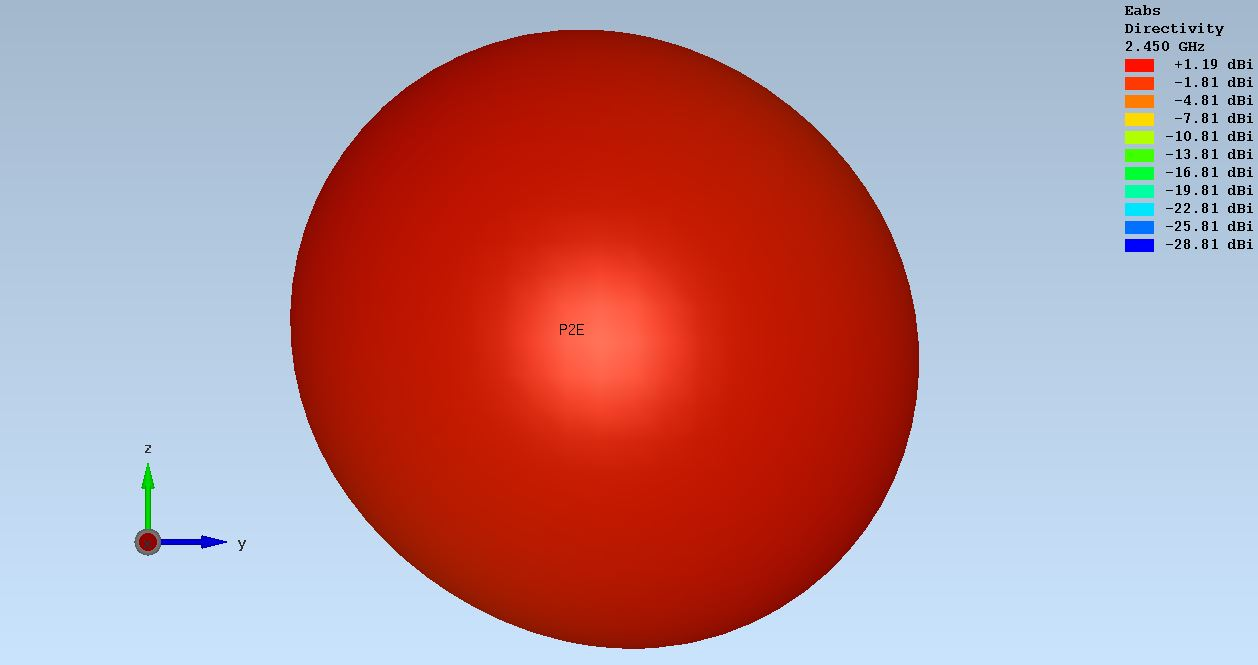
\includegraphics[width=0.9\textwidth]{content/bilder/Evaluation/Loop/L2/ohneABS/EM_Far_Field_Loop_Lambda2_ohneABS.JPG}
\captionof{figure}{Simulierte 3D Abstrahlcharakteristik eines $\lambda/2$ Loops}
\label{fig:sim_Loop_freiraum_3D}
\medskip
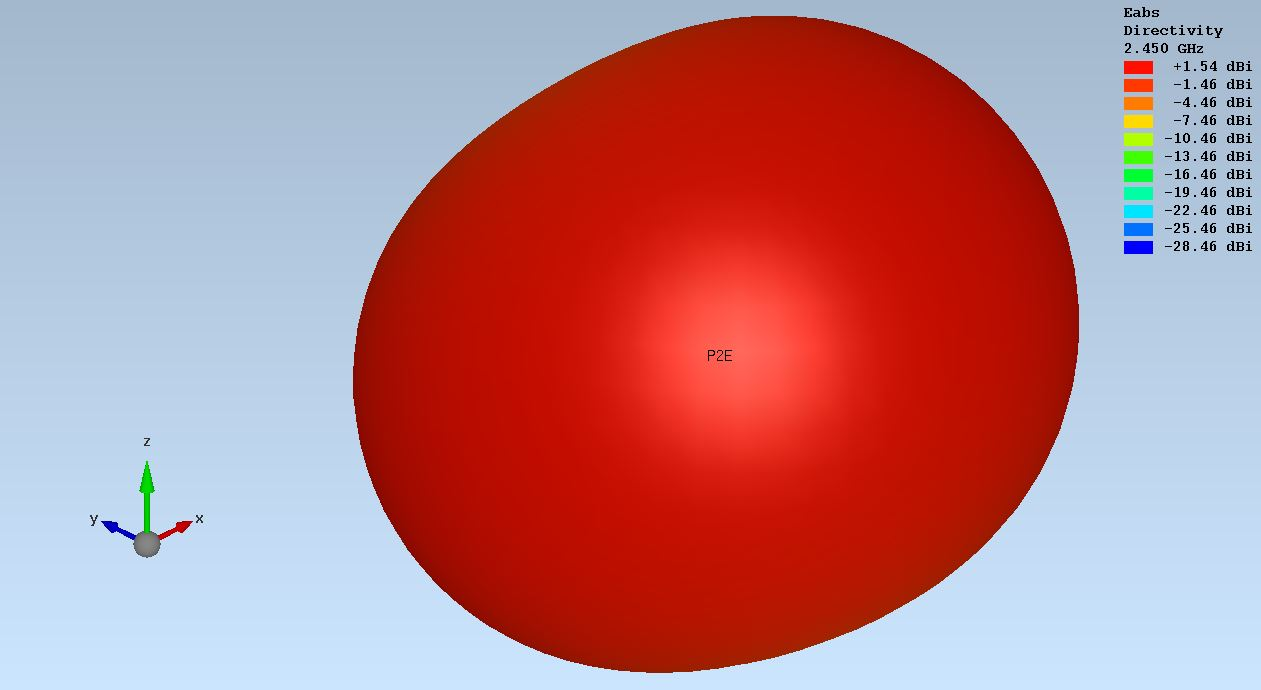
\includegraphics[width=0.9\textwidth]{content/bilder/Evaluation/Loop/L2/1ABS/EM_Far_Field_Loop_Lambda2_mitABS.JPG}
\captionof{figure}{Simulierte 3D Abstrahlcharakteristik eines $\lambda/2$ Loops mit einem ABS Stück im Nahfeld}
\label{fig:sim_Loop_freiraum_3D_1ABS}
\medskip
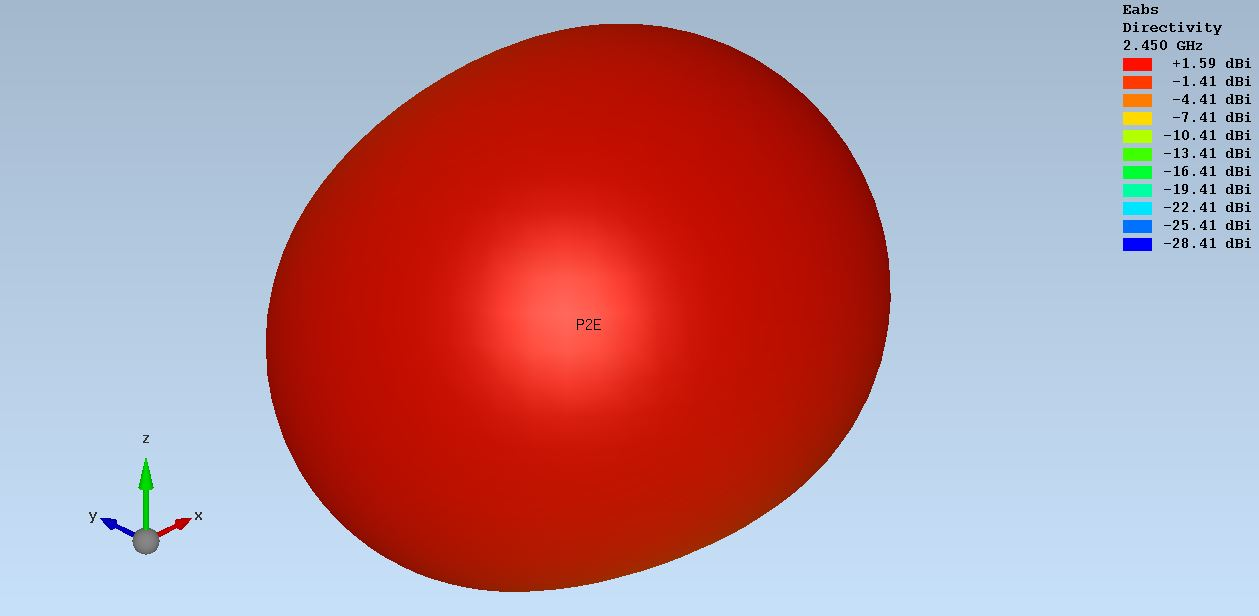
\includegraphics[width=0.9\textwidth]{content/bilder/Evaluation/Loop/L2/2ABS/EM_Far_Field_Loop_Lambda2_mit2ABS.JPG}
\captionof{figure}{Simulierte 3D Abstrahlcharakteristik eines $\lambda/2$ Loops mit einem ABS Stück im Nahfeld}
\label{fig:sim_Loop_freiraum_3D_2ABS}
%\medskip
%\includegraphics[width=0.6\textwidth, height=4cm]{Abb/V104.png}
%\captionof{figure}{Messwerte des Versuches IV}
}
%%%%%%%%%%%%%%%%%%%%%%%%%%%%%%%%%%%%%%%%%%%%%%%%%%%%%%
%%%%%%%%%%%%%%%%%%%%%%%%%%%%

%\newpage
\subsubsection{Simulationen einer Loop Antenne mit mehreren Windungen}
Im vorhergehenden Abschnitt Kapitel \ref{sec:SimL2Loop} sind anhand eines einfachen Modells die Eigenschaften einer Loop Antenne mit umliegendem Kunststoff gezeigt. Der Effekt des Kunststoffes war grösser als erwartet. Es ist ein Detuning wie bei einer Dipolantenne feststellbar. Dass das Detuning auch Chancen bildet, zeigen die drei folgenden Simulationen der Abbildungen von \ref{fig:S11_Loop_freiraum_1} bis \ref{fig:Smith_Loop_2ABS_6}. Es wurde immer dieselbe Antennenstruktur simuliert. Diese ist ähnlich wie eine RFID Spule aufgebaut. Drei lange, flache Windungen sind ineinander gedreht. Die Äusserste ist nicht Höher als 10mm und die Länge beträgt nicht mehr als 55mm. Die Simulation wurde drei mal durchgeführt. Die erste zeigt die Antenne im Freiraum, die zweite zeigt das Resonanzverhalten mit einem ABS Stück im Nahfeld und bei der dritten Simulation ist die Antennenstruktur zwischen zwei ABS Kunststoffstücken ersichtlich.\\

\textbf{Loop Antenne mit drei Windungen im Freiraum}\\
Wie zu erwarten war, sinkt die Resonanzfrequenz mit dem Kunststoff im Nahfeld. Die Abbildung \ref{fig:S11_Loop_freiraum_1} zeigt  die Rückflussdämpfung der Antennenstruktur. Das Bild \ref{fig:S11_Loop_freiraum_1} zeigt einen sehr schmalbandigen $S_{11}$ Verlauf. Die -10 dB Bandbreite beträgt 60MHz. Der maximale $S_{11}$ Wert liegt bei 3.3 GHz und weist -11dB aus. In Abbildung \ref{fig:S11_Loop_freiraum_1} zeigt eine Antennenimpedanz von (37+j375)$\Omega$. Dabei resultiert eine Abstrahleffizienz von ca. $\eta=2.5\%$
%%%%%%%%%%%%%%%%


\textbf{Loop Antenne mit drei Windungen und mit einem ABS Stück im Nahfeld}\\
Die beiden Abbildungen \ref{fig:S11_Loop_1ABS_3} und \ref{fig:Smith_Loop_1ABS_4} zeigen den dreifach Loop mit einem angrenzenden Kunststoff ABS Stück. Es zeigt, dass  die -10dB Bandbreite  60 MHz entspricht. Der maximale $S_{11}$ Wert zeigt sich bei 2.5 GHz mit einer Rückflussdämpfung von -14dB. Die simulierte Antennenimpedanz bei 2.45 GHz entspricht (19.7-j49)Ohm. Dies führt zu einer Abstrahleffizienz von 29$\%$.\\
%%%%%%%%%%%

\textbf{Loop Antenne mit drei Windungen mit zwei ABS Stücken im Nahfeld}\\
Ein Loop mit drei Windungen, der zwischen 2 ABS Kunststoffstücken positioniert ist, wird in der  Simulation xxx gezeigt.
\todo{welche Simulation}\\
Die maximale $S_{11}$ Dämpfung liegt bei 2.45 GHz. Die -10dB Bandbreite beträgt 60MHz. Die Effizienz liegt bei einer Frequenz von 2.45Ghz bei $45\%$. Die Abbildung \ref{fig:Smith_Loop_2ABS_6} zeigt das Smith Diagramm. Bei der Entwurfsfrequenz von 2.45GHz resultiert eine Antennenimpedanz $Z_{ant}$ von (31.6+5.5)Ohm.
Eine Richtwirkung von 4.7dBi zeigt das 3D Richtdigramm aus der Abbildung \ref{fig:sim_Loop_3Fach_2ABS_3D}.
%%%%%%%%%

%S11 Loop 3Winungen Freiraum 1 ABS 2 ABS
\begin{figure}[!ht]
	\centering
	\begingroup
	\inputencoding{latin1}
	% This file was created by matlab2tikz.
%
%The latest updates can be retrieved from
%  http://www.mathworks.com/matlabcentral/fileexchange/22022-matlab2tikz-matlab2tikz
%where you can also make suggestions and rate matlab2tikz.
%
\begin{tikzpicture}

\begin{axis}[%
width=6in,
height=4.5in,
at={(1.152in,0.655in)},
scale only axis,
separate axis lines,
every outer x axis line/.append style={black},
every x tick label/.append style={font=\color{black}},
xmin=1,
xmax=5.5,
xlabel={Frequenz in [GHz]},
xmajorgrids,
every outer y axis line/.append style={black},
every y tick label/.append style={font=\color{black}},
ymin=-25,
ymax=5,
ylabel={Amplitude in [dB]},
ymajorgrids,
axis background/.style={fill=white},
title={$\text{Simulation des  $|$S}_{\text{11}}\text{$|$ einer Loop Antnne mit drei Windungen im Freiraum, mit einem und zwei ABS St�cken}$},
legend style={at={(0.03,0.03)},anchor=south west,legend cell align=left,align=left,draw=black}
]
\addplot [color=red,solid]
  table[row sep=crcr]{%
1.25	-0.373559\\
1.26875	-0.358924\\
1.2875	-0.348329\\
1.30625	-0.343129\\
1.325	-0.335905\\
1.34375	-0.317614\\
1.3625	-0.285612\\
1.38125	-0.246618\\
1.4	-0.212418\\
1.41875	-0.191801\\
1.4375	-0.184682\\
1.45625	-0.182374\\
1.475	-0.173854\\
1.49375	-0.15382\\
1.5125	-0.126598\\
1.53125	-0.102821\\
1.55	-0.0914629\\
1.56875	-0.0931087\\
1.5875	-0.099205\\
1.60625	-0.0980195\\
1.625	-0.0834471\\
1.64375	-0.060162\\
1.6625	-0.0408736\\
1.68125	-0.0375283\\
1.7	-0.052723\\
1.71875	-0.0772242\\
1.7375	-0.0957804\\
1.75625	-0.0983247\\
1.775	-0.0892541\\
1.79375	-0.0877808\\
1.8125	-0.118629\\
1.83125	-0.198731\\
1.85	-0.326532\\
1.86875	-0.477912\\
1.8875	-0.611189\\
1.90625	-0.683424\\
1.925	-0.676789\\
1.94375	-0.622993\\
1.9625	-0.603026\\
1.98125	-0.699076\\
2	-0.88389\\
2.01875	-0.94798\\
2.0375	-0.740718\\
2.05625	-0.419355\\
2.075	-0.226239\\
2.09375	-0.275601\\
2.1125	-0.550567\\
2.13125	-0.936753\\
2.15	-1.2555\\
2.16875	-1.34662\\
2.1875	-1.17969\\
2.20625	-0.865819\\
2.225	-0.554049\\
2.24375	-0.342575\\
2.2625	-0.257672\\
2.28125	-0.268434\\
2.3	-0.31401\\
2.31875	-0.337747\\
2.3375	-0.316378\\
2.35625	-0.265327\\
2.375	-0.217803\\
2.39375	-0.197592\\
2.4125	-0.205075\\
2.43125	-0.221438\\
2.45	-0.22497\\
2.46875	-0.207331\\
2.4875	-0.177942\\
2.50625	-0.154339\\
2.525	-0.147825\\
2.54375	-0.155686\\
2.5625	-0.164617\\
2.58125	-0.161868\\
2.6	-0.145302\\
2.61875	-0.12437\\
2.6375	-0.111753\\
2.65625	-0.113071\\
2.675	-0.122784\\
2.69375	-0.129047\\
2.7125	-0.123535\\
2.73125	-0.108301\\
2.75	-0.0939024\\
2.76875	-0.0905425\\
2.7875	-0.0997079\\
2.80625	-0.112962\\
2.825	-0.118874\\
2.84375	-0.112704\\
2.8625	-0.100741\\
2.88125	-0.0953316\\
2.9	-0.10471\\
2.91875	-0.126039\\
2.9375	-0.147401\\
2.95625	-0.157693\\
2.975	-0.156747\\
2.99375	-0.156742\\
3.0125	-0.173044\\
3.03125	-0.211894\\
3.05	-0.264997\\
3.06875	-0.31614\\
3.0875	-0.356114\\
3.10625	-0.394262\\
3.125	-0.455798\\
3.14375	-0.566191\\
3.1625	-0.735237\\
3.18125	-0.954142\\
3.2	-1.2119\\
3.21875	-1.52491\\
3.2375	-1.96078\\
3.25625	-2.64033\\
3.275	-3.72429\\
3.29375	-5.40002\\
3.3125	-7.83066\\
3.33125	-10.6807\\
3.35	-11.4337\\
3.36875	-9.03765\\
3.3875	-6.47089\\
3.40625	-4.62781\\
3.425	-3.4143\\
3.44375	-2.64261\\
3.4625	-2.14076\\
3.48125	-1.76901\\
3.5	-1.4434\\
3.51875	-1.14683\\
3.5375	-0.90531\\
3.55625	-0.74502\\
3.575	-0.661264\\
3.59375	-0.614909\\
3.6125	-0.556312\\
3.63125	-0.460964\\
3.65	-0.346786\\
3.66875	-0.25626\\
3.6875	-0.220199\\
3.70625	-0.231936\\
3.725	-0.249055\\
3.74375	-0.22429\\
3.7625	-0.145795\\
3.78125	-0.0508175\\
3.8	0.00212449\\
3.81875	-0.0210494\\
3.8375	-0.098715\\
3.85625	-0.157831\\
3.875	-0.123191\\
3.89375	0.0124772\\
3.9125	0.160553\\
3.93125	0.17877\\
3.95	-0.0611085\\
3.96875	-0.623196\\
3.9875	-1.46933\\
4.00625	-2.39899\\
4.025	-2.98852\\
4.04375	-2.79194\\
4.0625	-1.871\\
4.08125	-0.864041\\
4.1	-0.167678\\
4.11875	-3.21041\\
4.1375	-0.551886\\
4.15625	-0.0626058\\
4.175	-0.0936687\\
4.19375	-0.278972\\
4.2125	-0.49339\\
4.23125	-0.685741\\
4.25	-0.842082\\
4.26875	-0.963947\\
4.2875	-1.05442\\
4.30625	-1.11458\\
4.325	-1.14635\\
4.34375	-1.15464\\
4.3625	-1.14573\\
4.38125	-1.12367\\
4.4	-1.08876\\
4.41875	-1.0397\\
4.4375	-0.977649\\
4.45625	-0.908426\\
4.475	-0.840634\\
4.49375	-0.781189\\
4.5125	-0.731672\\
4.53125	-0.688273\\
4.55	-0.645415\\
4.56875	-0.600279\\
4.5875	-0.554748\\
4.60625	-0.513487\\
4.625	-0.48001\\
4.64375	-0.454013\\
4.6625	-0.431992\\
4.68125	-0.410471\\
4.7	-0.389067\\
4.71875	-0.370858\\
4.7375	-0.359923\\
4.75625	-0.358319\\
4.775	-0.36516\\
4.79375	-0.378683\\
4.8125	-0.399591\\
4.83125	-0.432848\\
4.85	-0.486412\\
4.86875	-0.568138\\
4.8875	-0.683856\\
4.90625	-0.838892\\
4.925	-1.04233\\
4.94375	-1.31018\\
4.9625	-1.66269\\
4.98125	-2.1131\\
5	-2.64929\\
};
\addlegendentry{$\text{S}_{\text{11}}\text{ Frei Raum}$};

\addplot [color=blue,solid]
  table[row sep=crcr]{%
1.25	-0.862946\\
1.26875	-0.986593\\
1.2875	-1.15065\\
1.30625	-1.34748\\
1.325	-1.56338\\
1.34375	-1.7894\\
1.3625	-1.98101\\
1.38125	-2.08528\\
1.4	-2.08499\\
1.41875	-1.99653\\
1.4375	-1.84613\\
1.45625	-1.64651\\
1.475	-1.46628\\
1.49375	-1.38908\\
1.5125	-1.35956\\
1.53125	-1.11083\\
1.55	-0.858725\\
1.56875	-1.57492\\
1.5875	-1.57931\\
1.60625	-1.12512\\
1.625	-0.776487\\
1.64375	-0.69724\\
1.6625	-0.642895\\
1.68125	-0.572594\\
1.7	-0.549408\\
1.71875	-0.520092\\
1.7375	-0.48578\\
1.75625	-0.47316\\
1.775	-0.453195\\
1.79375	-0.433652\\
1.8125	-0.42625\\
1.83125	-0.412229\\
1.85	-0.40116\\
1.86875	-0.397083\\
1.8875	-0.387527\\
1.90625	-0.382143\\
1.925	-0.380506\\
1.94375	-0.374676\\
1.9625	-0.373543\\
1.98125	-0.373984\\
2	-0.371604\\
2.01875	-0.374074\\
2.0375	-0.376731\\
2.05625	-0.378059\\
2.075	-0.38428\\
2.09375	-0.39005\\
2.1125	-0.396244\\
2.13125	-0.407577\\
2.15	-0.418723\\
2.16875	-0.4326\\
2.1875	-0.452529\\
2.20625	-0.473887\\
2.225	-0.501512\\
2.24375	-0.537794\\
2.2625	-0.579767\\
2.28125	-0.634715\\
2.3	-0.705519\\
2.31875	-0.79309\\
2.3375	-0.90995\\
2.35625	-1.06445\\
2.375	-1.26921\\
2.39375	-1.55466\\
2.4125	-1.95651\\
2.43125	-2.53625\\
2.45	-3.40923\\
2.46875	-4.7594\\
2.4875	-6.91342\\
2.50625	-10.41\\
2.525	-14.6554\\
2.54375	-12.59\\
2.5625	-8.53295\\
2.58125	-5.93846\\
2.6	-4.333\\
2.61875	-3.29678\\
2.6375	-2.60425\\
2.65625	-2.13498\\
2.675	-1.79991\\
2.69375	-1.55641\\
2.7125	-1.39013\\
2.73125	-1.26349\\
2.75	-1.16986\\
2.76875	-1.12461\\
2.7875	-1.0893\\
2.80625	-1.0699\\
2.825	-1.11641\\
2.84375	-1.16797\\
2.8625	-1.23904\\
2.88125	-1.53932\\
2.9	-2.01287\\
2.91875	-2.19509\\
2.9375	-1.97875\\
2.95625	-1.79999\\
2.975	-1.84507\\
2.99375	-1.98489\\
3.0125	-2.14692\\
3.03125	-2.34831\\
3.05	-2.56676\\
3.06875	-2.76847\\
3.0875	-2.94609\\
3.10625	-3.08183\\
3.125	-3.14942\\
3.14375	-3.14685\\
3.1625	-3.08353\\
3.18125	-2.96462\\
3.2	-2.8077\\
3.21875	-2.63515\\
3.2375	-2.45564\\
3.25625	-2.2786\\
3.275	-2.11543\\
3.29375	-1.966\\
3.3125	-1.83144\\
3.33125	-1.71651\\
3.35	-1.61809\\
3.36875	-1.5358\\
3.3875	-1.47304\\
3.40625	-1.42734\\
3.425	-1.39988\\
3.44375	-1.39524\\
3.4625	-1.41378\\
3.48125	-1.4606\\
3.5	-1.54474\\
3.51875	-1.67341\\
3.5375	-1.86102\\
3.55625	-2.12832\\
3.575	-2.49711\\
3.59375	-2.99564\\
3.6125	-3.64801\\
3.63125	-4.44308\\
3.65	-5.29009\\
3.66875	-5.9709\\
3.6875	-6.20788\\
3.70625	-5.91613\\
3.725	-5.2926\\
3.74375	-4.58585\\
3.7625	-3.93281\\
3.78125	-3.3793\\
3.8	-2.93035\\
3.81875	-2.56796\\
3.8375	-2.27963\\
3.85625	-2.07145\\
3.875	-1.92344\\
3.89375	-1.78457\\
3.9125	-1.63984\\
3.93125	-1.51301\\
3.95	-1.41006\\
3.96875	-1.32203\\
3.9875	-1.24833\\
4.00625	-1.18672\\
4.025	-1.13302\\
4.04375	-1.08779\\
4.0625	-1.04953\\
4.08125	-1.01628\\
4.1	-0.988817\\
4.11875	-0.965986\\
4.1375	-0.946869\\
4.15625	-0.932233\\
4.175	-0.921119\\
4.19375	-0.913226\\
4.2125	-0.909226\\
4.23125	-0.908341\\
4.25	-0.91069\\
4.26875	-0.916849\\
4.2875	-0.926238\\
4.30625	-0.939305\\
4.325	-0.956587\\
4.34375	-0.977753\\
4.3625	-1.00358\\
4.38125	-1.03464\\
4.4	-1.07098\\
4.41875	-1.11379\\
4.4375	-1.16385\\
4.45625	-1.22178\\
4.475	-1.28939\\
4.49375	-1.36804\\
4.5125	-1.4593\\
4.53125	-1.56613\\
4.55	-1.6911\\
4.56875	-1.83765\\
4.5875	-2.01094\\
4.60625	-2.21623\\
4.625	-2.46078\\
4.64375	-2.75452\\
4.6625	-3.10878\\
4.68125	-3.53937\\
4.7	-4.06734\\
4.71875	-4.71905\\
4.7375	-5.53183\\
4.75625	-6.55728\\
4.775	-7.8676\\
4.79375	-9.57416\\
4.8125	-11.8524\\
4.83125	-14.9685\\
4.85	-18.9631\\
4.86875	-20.416\\
4.8875	-16.8744\\
4.90625	-13.4765\\
4.925	-11.0227\\
4.94375	-9.24075\\
4.9625	-7.91472\\
4.98125	-6.90965\\
5	-6.14829\\
};
\addlegendentry{$\text{S}_{\text{11}}\text{ mit ABS}$};

\addplot [color=green,solid]
  table[row sep=crcr]{%
1.5	-1.79009\\
1.5325	-1.11179\\
1.565	-0.603335\\
1.5975	-0.545151\\
1.63	-0.478543\\
1.6625	-0.418912\\
1.695	-0.415815\\
1.7275	-0.357009\\
1.76	-0.374919\\
1.7925	-0.326421\\
1.825	-0.347223\\
1.8575	-0.316737\\
1.89	-0.33214\\
1.9225	-0.324789\\
1.955	-0.334899\\
1.9875	-0.354136\\
2.02	-0.36813\\
2.0525	-0.419845\\
2.085	-0.45975\\
2.1175	-0.564675\\
2.15	-0.683369\\
2.1825	-0.921181\\
2.215	-1.29127\\
2.2475	-2.01956\\
2.28	-3.4867\\
2.3125	-6.82331\\
2.345	-12.2621\\
2.3775	-7.98678\\
2.41	-4.28423\\
2.4425	-2.60881\\
2.475	-1.79087\\
2.5075	-1.35292\\
2.54	-1.09939\\
2.5725	-0.973714\\
2.605	-0.889634\\
2.6375	-0.906402\\
2.67	-0.922162\\
2.7025	-1.09531\\
2.735	-1.3874\\
2.7675	-2.3422\\
2.8	-2.19124\\
2.8325	-1.91325\\
2.865	-2.16685\\
2.8975	-2.49648\\
2.93	-2.86691\\
2.9625	-3.122\\
2.995	-3.21206\\
3.0275	-3.09741\\
3.06	-2.86273\\
3.0925	-2.56851\\
3.125	-2.2902\\
3.1575	-2.0475\\
3.19	-1.85933\\
3.2225	-1.7302\\
3.255	-1.66067\\
3.2875	-1.67169\\
3.32	-1.77255\\
3.3525	-2.02732\\
3.385	-2.50337\\
3.4175	-3.37938\\
3.45	-4.85267\\
3.4825	-6.91882\\
3.515	-8.03498\\
3.5475	-6.75778\\
3.58	-4.96027\\
3.6125	-3.67183\\
3.645	-2.85584\\
3.6775	-2.46181\\
3.71	-2.22184\\
3.7425	-1.84728\\
3.775	-1.57549\\
3.8075	-1.3872\\
3.84	-1.25455\\
3.8725	-1.15722\\
3.905	-1.08396\\
3.9375	-1.03269\\
3.97	-0.996049\\
4.0025	-0.975556\\
4.035	-0.969049\\
4.0675	-0.97624\\
4.1	-1.00104\\
4.1325	-1.04163\\
4.165	-1.10642\\
4.1975	-1.19622\\
4.23	-1.32235\\
4.2625	-1.49422\\
4.295	-1.7288\\
4.3275	-2.05261\\
4.36	-2.50126\\
4.3925	-3.13827\\
4.425	-4.05604\\
4.4575	-5.41992\\
4.49	-7.51597\\
4.5225	-10.9551\\
4.555	-17.4351\\
4.5875	-22.3464\\
4.62	-13.7073\\
4.6525	-9.50124\\
4.685	-7.1299\\
4.7175	-5.67546\\
4.75	-4.76452\\
4.7825	-4.21457\\
4.815	-3.92619\\
4.8475	-3.85404\\
4.88	-3.97325\\
4.9125	-4.2869\\
4.945	-4.77488\\
4.9775	-5.29045\\
5.01	-5.43417\\
};
\addlegendentry{$\text{S}_{\text{11}}\text{ mit 2 ABS}$};

\end{axis}
\end{tikzpicture}%
	\endgroup
	\caption{Vergleich des $S_{11}$ Werts einer Loop Antenne}
	\label{S11_Loop_Vergleich_Simulation}
\end{figure}
%%%%%%%%%%%%
%Impedanz
%real und imag
%Loop Mit 3Windungen
\begin{figure}[!ht]
	\centering
	\begingroup
	\inputencoding{latin1}
	% This file was created by matlab2tikz.
%
%The latest updates can be retrieved from
%  http://www.mathworks.com/matlabcentral/fileexchange/22022-matlab2tikz-matlab2tikz
%where you can also make suggestions and rate matlab2tikz.
%
\definecolor{mycolor1}{rgb}{1.00000,1.00000,0.00000}%
\definecolor{mycolor2}{rgb}{1.00000,0.00000,1.00000}%
%
\begin{tikzpicture}

\begin{axis}[%
width=6in,
height=4.5in,
at={(1.54in,0.88in)},
scale only axis,
separate axis lines,
every outer x axis line/.append style={black},
every x tick label/.append style={font=\color{black}},
xmin=1.95,
xmax=3.15,
xlabel={Frequenz in [GHz]},
xmajorgrids,
every outer y axis line/.append style={black},
every y tick label/.append style={font=\color{black}},
ymin=-3.50638977635782,
ymax=4.96006389776358,
ylabel={Impedanz [Ohm]},
ymajorgrids,
axis background/.style={fill=white},
title={Impedanz der Loop Antenne mit drei Windungen im Freiraum, mit einem und zwei ABS-St�cken},
legend style={legend cell align=left,align=left,draw=black}
]
\addplot [color=red,very thick,solid]
  table[row sep=crcr]{%
1.25	0.00140942\\
1.26875	0.00160261\\
1.2875	0.00189237\\
1.30625	0.00231306\\
1.325	0.00284721\\
1.34375	0.00341966\\
1.3625	0.00394862\\
1.38125	0.0044412\\
1.4	0.00507666\\
1.41875	0.00622096\\
1.4375	0.00834104\\
1.45625	0.0118396\\
1.475	0.0169911\\
1.49375	0.0244527\\
1.5125	0.0376391\\
1.53125	0.0755416\\
1.55	0.352198\\
1.56875	2.87003\\
1.5875	0.157409\\
1.60625	0.0483954\\
1.625	0.0195102\\
1.64375	0.00796397\\
1.6625	0.0033813\\
1.68125	0.00207378\\
1.7	0.00204684\\
1.71875	0.00218836\\
1.7375	0.0020336\\
1.75625	0.00158748\\
1.775	0.0011035\\
1.79375	0.00083509\\
1.8125	0.000875308\\
1.83125	0.0011537\\
1.85	0.00152452\\
1.86875	0.00184926\\
1.8875	0.00203757\\
1.90625	0.00205945\\
1.925	0.0019503\\
1.94375	0.00182518\\
1.9625	0.00190628\\
1.98125	0.00249969\\
2	0.00365117\\
2.01875	0.00450666\\
2.0375	0.00406584\\
2.05625	0.00273157\\
2.075	0.00181001\\
2.09375	0.00276414\\
2.1125	0.00684524\\
2.13125	0.0136993\\
2.15	0.0200725\\
2.16875	0.0225016\\
2.1875	0.0207561\\
2.20625	0.0167109\\
2.225	0.0122931\\
2.24375	0.00905648\\
2.2625	0.00824372\\
2.28125	0.0103092\\
2.3	0.0141233\\
2.31875	0.0173886\\
2.3375	0.0185614\\
2.35625	0.0180094\\
2.375	0.0175061\\
2.39375	0.0191332\\
2.4125	0.0239908\\
2.43125	0.031028\\
2.45	0.037528\\
2.46875	0.0416078\\
2.4875	0.0442499\\
2.50625	0.0494724\\
2.525	0.0632956\\
2.54375	0.0911262\\
2.5625	0.134001\\
2.58125	0.19024\\
2.6	0.270344\\
2.61875	0.439584\\
2.6375	1.05089\\
2.65625	4.84373\\
2.675	4.32308\\
2.69375	1.25569\\
2.7125	0.520483\\
2.73125	0.243256\\
2.75	0.125314\\
2.76875	0.0782228\\
2.7875	0.0603936\\
2.80625	0.0513124\\
2.825	0.0423962\\
2.84375	0.0322569\\
2.8625	0.0232756\\
2.88125	0.0178549\\
2.9	0.0160912\\
2.91875	0.0162044\\
2.9375	0.0161595\\
2.95625	0.0148984\\
2.975	0.0127589\\
2.99375	0.0109287\\
3.0125	0.0103053\\
3.03125	0.0108255\\
3.05	0.0117197\\
3.06875	0.0121861\\
3.0875	0.0119497\\
3.10625	0.0114094\\
3.125	0.0112423\\
3.14375	0.0118137\\
3.1625	0.0129565\\
3.18125	0.0142026\\
3.2	0.0151627\\
3.21875	0.0158076\\
3.2375	0.0164746\\
3.25625	0.017578\\
3.275	0.0193191\\
3.29375	0.0216566\\
3.3125	0.0244518\\
3.33125	0.0276028\\
3.35	0.0311219\\
3.36875	0.0351994\\
3.3875	0.0403095\\
3.40625	0.0474003\\
3.425	0.0581302\\
3.44375	0.0748916\\
3.4625	0.10027\\
3.48125	0.137089\\
3.5	0.193299\\
3.51875	0.298635\\
3.5375	0.55662\\
3.55625	1.11974\\
3.575	0.961198\\
3.59375	0.472777\\
3.6125	0.253973\\
3.63125	0.139016\\
3.65	0.0712985\\
3.66875	0.0366427\\
3.6875	0.0228983\\
3.70625	0.0186838\\
3.725	0.0164996\\
3.74375	0.0126648\\
3.7625	0.00703784\\
3.78125	0.00206217\\
3.8	-7.17e-05\\
3.81875	0.000597805\\
3.8375	0.0024291\\
3.85625	0.00347008\\
3.875	0.00244737\\
3.89375	-0.000219598\\
3.9125	-0.00240982\\
3.93125	-0.00222609\\
3.95	0.000631588\\
3.96875	0.00549627\\
3.9875	0.0116112\\
4.00625	0.0181888\\
4.025	0.0236656\\
4.04375	0.0246075\\
4.0625	0.0177309\\
4.08125	0.00806638\\
4.1	0.000704039\\
4.11875	0.0141972\\
4.1375	0.00270407\\
4.15625	0.000261864\\
4.175	0.000345346\\
4.19375	0.000933381\\
4.2125	0.00153493\\
4.23125	0.00202946\\
4.25	0.00242881\\
4.26875	0.00278321\\
4.2875	0.00313698\\
4.30625	0.00351863\\
4.325	0.00394921\\
4.34375	0.00445136\\
4.3625	0.00504902\\
4.38125	0.00575732\\
4.4	0.00657175\\
4.41875	0.00747165\\
4.4375	0.00844604\\
4.45625	0.00953012\\
4.475	0.0108268\\
4.49375	0.0124949\\
4.5125	0.0147072\\
4.53125	0.0176152\\
4.55	0.021384\\
4.56875	0.0263573\\
4.5875	0.0333872\\
4.60625	0.0444196\\
4.625	0.063805\\
4.64375	0.102352\\
4.6625	0.194274\\
4.68125	0.499773\\
4.7	1.93442\\
4.71875	0.965318\\
4.7375	0.252163\\
4.75625	0.105216\\
4.775	0.0569172\\
4.79375	0.0357011\\
4.8125	0.0246405\\
4.83125	0.0183549\\
4.85	0.0146832\\
4.86875	0.0125264\\
4.8875	0.0112324\\
4.90625	0.0104206\\
4.925	0.00990686\\
4.94375	0.00962936\\
4.9625	0.00957243\\
4.98125	0.00971338\\
5	0.0100081\\
};
\addlegendentry{Realanteil im Freiraum};

\addplot [color=blue,very thick,solid]
  table[row sep=crcr]{%
1.25	0.0278779\\
1.26875	0.0371202\\
1.2875	0.0470929\\
1.30625	0.0579045\\
1.325	0.0696987\\
1.34375	0.0827304\\
1.3625	0.097453\\
1.38125	0.11457\\
1.4	0.135045\\
1.41875	0.160119\\
1.4375	0.191482\\
1.45625	0.231854\\
1.475	0.286551\\
1.49375	0.367417\\
1.5125	0.504325\\
1.53125	0.793704\\
1.55	1.79395\\
1.56875	-4.30526\\
1.5875	-1.16232\\
1.60625	-0.651174\\
1.625	-0.447442\\
1.64375	-0.335288\\
1.6625	-0.263332\\
1.68125	-0.213292\\
1.7	-0.176684\\
1.71875	-0.148693\\
1.7375	-0.126248\\
1.75625	-0.107339\\
1.775	-0.0907637\\
1.79375	-0.075913\\
1.8125	-0.0625186\\
1.83125	-0.050418\\
1.85	-0.0394321\\
1.86875	-0.0293418\\
1.8875	-0.0199075\\
1.90625	-0.01089\\
1.925	-0.00206447\\
1.94375	0.00676287\\
1.9625	0.0157018\\
1.98125	0.0246226\\
2	0.0329699\\
2.01875	0.0403152\\
2.0375	0.0475683\\
2.05625	0.0561668\\
2.075	0.0666887\\
2.09375	0.0787831\\
2.1125	0.0909221\\
2.13125	0.100319\\
2.15	    0.105264\\
2.16875	0.107813\\
2.1875	0.111559\\
2.20625	0.118493\\
2.225	0.129024\\
2.24375	0.142802\\
2.2625	0.158836\\
2.28125	0.175392\\
2.3	    0.190747\\
2.31875	0.20479\\
2.3375	0.219401\\
2.35625	0.236961\\
2.375	0.258885\\
2.39375	0.285054\\
2.4125	0.313935\\
2.43125	0.343905\\
2.45	    0.375522\\
2.46875	0.412447\\
2.4875	0.459966\\
2.50625	0.522975\\
2.525	0.604518\\
2.54375	0.705444\\
2.5625	0.828659\\
2.58125	0.991092\\
2.6	1.24122\\
2.61875	1.69543\\
2.6375	2.65735\\
2.65625	3.70763\\
2.675	-3.44854\\
2.69375	-2.62167\\
2.7125	-1.84022\\
2.73125	-1.37455\\
2.75	-1.06817\\
2.76875	-0.861285\\
2.7875	-0.721099\\
2.80625	-0.624052\\
2.825	-0.552723\\
2.84375	-0.495047\\
2.8625	-0.444578\\
2.88125	-0.399835\\
2.9	-0.361562\\
2.91875	-0.330024\\
2.9375	-0.30409\\
2.95625	-0.281689\\
2.975	-0.260857\\
2.99375	-0.240726\\
3.0125	-0.221648\\
3.03125	-0.20437\\
3.05	-0.189179\\
3.06875	-0.175634\\
3.0875	-0.162849\\
3.10625	-0.150076\\
3.125	-0.137176\\
3.14375	-0.124537\\
3.1625	-0.112584\\
3.18125	-0.101387\\
3.2	-0.0905976\\
3.21875	-0.0796646\\
3.2375	-0.0681913\\
3.25625	-0.0561309\\
3.275	-0.0436487\\
3.29375	-0.0308558\\
3.3125	-0.0176688\\
3.33125	-0.00380146\\
3.35	0.0112115\\
3.36875	0.0280152\\
3.3875	0.0474523\\
3.40625	0.0705409\\
3.425	0.0983006\\
3.44375	0.131385\\
3.4625	0.170146\\
3.48125	0.21667\\
3.5	0.278433\\
3.51875	0.368524\\
3.5375	0.472915\\
3.55625	0.228779\\
3.575	-0.581892\\
3.59375	-0.665521\\
3.6125	-0.574523\\
3.63125	-0.490272\\
3.65	-0.413632\\
3.66875	-0.346977\\
3.6875	-0.295498\\
3.70625	-0.259109\\
3.725	-0.234065\\
3.74375	-0.215398\\
3.7625	-0.198452\\
3.78125	-0.180951\\
3.8	-0.163767\\
3.81875	-0.148888\\
3.8375	-0.137363\\
3.85625	-0.12879\\
3.875	-0.121454\\
3.89375	-0.11308\\
3.9125	-0.102629\\
3.93125	-0.0911726\\
3.95	-0.0804801\\
3.96875	-0.0717178\\
3.9875	-0.065532\\
4.00625	-0.06262\\
4.025	-0.0639333\\
4.04375	-0.0693676\\
4.0625	-0.0744574\\
4.08125	-0.0746358\\
4.1	-0.0338665\\
4.11875	-0.0362337\\
4.1375	-0.0418835\\
4.15625	-0.0336612\\
4.175	-0.0265027\\
4.19375	-0.0201553\\
4.2125	-0.0142381\\
4.23125	-0.00847443\\
4.25	-0.0026857\\
4.26875	0.00322891\\
4.2875	0.00932471\\
4.30625	0.015643\\
4.325	0.022228\\
4.34375	0.0291284\\
4.3625	0.0363922\\
4.38125	0.0440682\\
4.4	0.0522209\\
4.41875	0.0609586\\
4.4375	0.070457\\
4.45625	0.0809603\\
4.475	0.0927608\\
4.49375	0.10618\\
4.5125	0.121591\\
4.53125	0.139522\\
4.55	0.160854\\
4.56875	0.187094\\
4.5875	0.220753\\
4.60625	0.265993\\
4.625	0.330156\\
4.64375	0.427803\\
4.6625	0.592198\\
4.68125	0.897816\\
4.7	0.759597\\
4.71875	-1.15235\\
4.7375	-0.736747\\
4.75625	-0.491554\\
4.775	-0.360176\\
4.79375	-0.279581\\
4.8125	-0.224703\\
4.83125	-0.184461\\
4.85	-0.1534\\
4.86875	-0.128535\\
4.8875	-0.108027\\
4.90625	-0.0906337\\
4.925	-0.0754785\\
4.94375	-0.0619633\\
4.9625	-0.0496984\\
4.98125	-0.0384289\\
5	-0.0279675\\
};
\addlegendentry{Imagin�ranteil im Freiraum};

\addplot [color=green,very thick,solid]
  table[row sep=crcr]{%
1.25	0.014102\\
1.26875	0.0110641\\
1.2875	0.00921524\\
1.30625	0.00800528\\
1.325	0.00716401\\
1.34375	0.00663107\\
1.3625	0.00629721\\
1.38125	0.00608329\\
1.4	0.0059865\\
1.41875	0.00601151\\
1.4375	0.00612468\\
1.45625	0.00623312\\
1.475	0.00649956\\
1.49375	0.00727917\\
1.5125	0.0083666\\
1.53125	0.00822564\\
1.55	0.00782621\\
1.56875	0.0171289\\
1.5875	0.0181604\\
1.60625	0.0144681\\
1.625	0.0121357\\
1.64375	0.0132915\\
1.6625	0.0145918\\
1.68125	0.015654\\
1.7	0.0181509\\
1.71875	0.0206718\\
1.7375	0.0235736\\
1.75625	0.028228\\
1.775	0.0334393\\
1.79375	0.0404328\\
1.8125	0.050951\\
1.83125	0.064477\\
1.85	0.0852157\\
1.86875	0.118516\\
1.8875	0.171578\\
1.90625	0.272864\\
1.925	0.482875\\
1.94375	0.977707\\
1.9625	2.02682\\
1.98125	2.02187\\
2	0.993513\\
2.01875	0.49265\\
2.0375	0.28375\\
2.05625	0.180594\\
2.075	0.125409\\
2.09375	0.0921799\\
2.1125	0.0703421\\
2.13125	0.0560299\\
2.15	0.0456969\\
2.16875	0.0380744\\
2.1875	0.0326078\\
2.20625	0.0282869\\
2.225	0.0249742\\
2.24375	0.0225116\\
2.2625	0.0204977\\
2.28125	0.0189915\\
2.3	0.0179088\\
2.31875	0.0170732\\
2.3375	0.0165735\\
2.35625	0.0163603\\
2.375	0.0163688\\
2.39375	0.0166942\\
2.4125	0.0173371\\
2.43125	0.0183199\\
2.45	    0.0197861\\
2.46875	0.0218606\\
2.4875	0.0247459\\
2.50625	0.0288459\\
2.525	0.0347959\\
2.54375	0.0436875\\
2.5625	0.0576437\\
2.58125	0.0810093\\
2.6	0.122713\\
2.61875	0.20004\\
2.6375	0.322735\\
2.65625	0.374639\\
2.675	0.260447\\
2.69375	0.14794\\
2.7125	0.0876527\\
2.73125	0.0563427\\
2.75	0.0386168\\
2.76875	0.0286164\\
2.7875	0.0221383\\
2.80625	0.01761\\
2.825	0.0151339\\
2.84375	0.0133208\\
2.8625	0.0118428\\
2.88125	0.012382\\
2.9	0.0143452\\
2.91875	0.0145731\\
2.9375	0.012003\\
2.95625	0.00955803\\
2.975	0.00854851\\
2.99375	0.00814769\\
3.0125	0.00790795\\
3.03125	0.00787284\\
3.05	0.00797899\\
3.06875	0.00815305\\
3.0875	0.00842816\\
3.10625	0.00881314\\
3.125	0.0092839\\
3.14375	0.00986744\\
3.1625	0.0105997\\
3.18125	0.0114842\\
3.2	0.0125664\\
3.21875	0.0139272\\
3.2375	0.0156241\\
3.25625	0.0177842\\
3.275	0.0206337\\
3.29375	0.024442\\
3.3125	0.029726\\
3.33125	0.0374485\\
3.35	0.0492558\\
3.36875	0.0687186\\
3.3875	0.104048\\
3.40625	0.175529\\
3.425	0.334422\\
3.44375	0.589985\\
3.4625	0.506587\\
3.48125	0.254577\\
3.5	0.1325\\
3.51875	0.0788812\\
3.5375	0.0525596\\
3.55625	0.0382897\\
3.575	0.0299177\\
3.59375	0.0247439\\
3.6125	0.0214739\\
3.63125	0.0193955\\
3.65	0.018114\\
3.66875	0.0174102\\
3.6875	0.0171442\\
3.70625	0.0172259\\
3.725	0.0176141\\
3.74375	0.0182925\\
3.7625	0.0192447\\
3.78125	0.0204896\\
3.8	0.0220858\\
3.81875	0.0240685\\
3.8375	0.0266097\\
3.85625	0.0300999\\
3.875	0.0345169\\
3.89375	0.0392926\\
3.9125	0.044571\\
3.93125	0.0513388\\
3.95	0.0602378\\
3.96875	0.0718598\\
3.9875	0.0875521\\
4.00625	0.109087\\
4.025	0.139355\\
4.04375	0.183576\\
4.0625	0.249838\\
4.08125	0.351581\\
4.1	0.50634\\
4.11875	0.714529\\
4.1375	0.897226\\
4.15625	0.893648\\
4.175	0.711052\\
4.19375	0.507684\\
4.2125	0.357276\\
4.23125	0.257737\\
4.25	0.192286\\
4.26875	0.148379\\
4.2875	0.117951\\
4.30625	0.0961856\\
4.325	0.0802361\\
4.34375	0.0682253\\
4.3625	0.0589995\\
4.38125	0.0518105\\
4.4	0.0461026\\
4.41875	0.0415298\\
4.4375	0.0378407\\
4.45625	0.0348309\\
4.475	0.0323788\\
4.49375	0.0303831\\
4.5125	0.0287575\\
4.53125	0.0274576\\
4.55	0.0264379\\
4.56875	0.0256619\\
4.5875	0.0251174\\
4.60625	0.0247863\\
4.625	0.024659\\
4.64375	0.0247429\\
4.6625	0.0250399\\
4.68125	0.0255636\\
4.7	0.0263428\\
4.71875	0.0274062\\
4.7375	0.028801\\
4.75625	0.0305958\\
4.775	0.0328718\\
4.79375	0.0357449\\
4.8125	0.0393706\\
4.83125	0.0439393\\
4.85	0.0496906\\
4.86875	0.0568927\\
4.8875	0.0657444\\
4.90625	0.0761854\\
4.925	0.0874948\\
4.94375	0.0976675\\
4.9625	0.103484\\
4.98125	0.101935\\
5	0.092888\\
};
\addlegendentry{Realanteil mit 1 ABS};

\addplot [color=black,very thick,solid]
  table[row sep=crcr]{%
1.25	-0.107434\\
1.26875	-0.0846181\\
1.2875	-0.0664229\\
1.30625	-0.0513562\\
1.325	-0.0383638\\
1.34375	-0.0268366\\
1.3625	-0.0164046\\
1.38125	-0.00673645\\
1.4	0.00240914\\
1.41875	0.0111833\\
1.4375	0.0196817\\
1.45625	0.0280822\\
1.475	0.0366668\\
1.49375	0.0451377\\
1.5125	0.0530924\\
1.53125	0.0624438\\
1.55	0.0733528\\
1.56875	0.0821992\\
1.5875	0.0852519\\
1.60625	0.0923171\\
1.625	0.104709\\
1.64375	0.11797\\
1.6625	0.130528\\
1.68125	0.145036\\
1.7	0.160949\\
1.71875	0.177869\\
1.7375	0.197835\\
1.75625	0.220393\\
1.775	0.246027\\
1.79375	0.277341\\
1.8125	0.314344\\
1.83125	0.359585\\
1.85	0.418184\\
1.86875	0.492827\\
1.8875	0.59404\\
1.90625	0.737325\\
1.925	0.931292\\
1.94375	1.14436\\
1.9625	0.778023\\
1.98125	-0.779926\\
2	-1.15503\\
2.01875	-0.94838\\
2.0375	-0.756048\\
2.05625	-0.616491\\
2.075	-0.515188\\
2.09375	-0.440923\\
2.1125	-0.383213\\
2.13125	-0.337422\\
2.15	-0.300463\\
2.16875	-0.269371\\
2.1875	-0.243066\\
2.20625	-0.220451\\
2.225	-0.200445\\
2.24375	-0.182751\\
2.2625	-0.166837\\
2.28125	-0.152233\\
2.3	-0.138837\\
2.31875	-0.126329\\
2.3375	-0.11447\\
2.35625	-0.103194\\
2.375	-0.0922699\\
2.39375	-0.0815336\\
2.4125	-0.0708938\\
2.43125	-0.0601305\\
2.45	-0.0490488\\
2.46875	-0.037459\\
2.4875	-0.025041\\
2.50625	-0.0114014\\
2.525	0.00394013\\
2.54375	0.0216674\\
2.5625	0.0426761\\
2.58125	0.0676565\\
2.6	0.0951206\\
2.61875	0.112671\\
2.6375	0.064727\\
2.65625	-0.112339\\
2.675	-0.239052\\
2.69375	-0.243016\\
2.7125	-0.212254\\
2.73125	-0.182569\\
2.75	-0.157651\\
2.76875	-0.1375\\
2.7875	-0.12147\\
2.80625	-0.107511\\
2.825	-0.0954472\\
2.84375	-0.0853728\\
2.8625	-0.0756173\\
2.88125	-0.066381\\
2.9	-0.059957\\
2.91875	-0.0563594\\
2.9375	-0.052111\\
2.95625	-0.0456808\\
2.975	-0.0388792\\
2.99375	-0.0325713\\
3.0125	-0.0264899\\
3.03125	-0.020509\\
3.05	-0.0146478\\
3.06875	-0.00880512\\
3.0875	-0.00289619\\
3.10625	0.00309938\\
3.125	0.00924573\\
3.14375	0.0156322\\
3.1625	0.0223123\\
3.18125	0.0293679\\
3.2	0.0369336\\
3.21875	0.0451292\\
3.2375	0.0541182\\
3.25625	0.0641697\\
3.275	0.0755857\\
3.29375	0.0887973\\
3.3125	0.104511\\
3.33125	0.123666\\
3.35	0.147714\\
3.36875	0.179015\\
3.3875	0.220486\\
3.40625	0.272883\\
3.425	0.308149\\
3.44375	0.140918\\
3.4625	-0.234196\\
3.48125	-0.292416\\
3.5	-0.235012\\
3.51875	-0.180905\\
3.5375	-0.140152\\
3.55625	-0.109416\\
3.575	-0.0854199\\
3.59375	-0.0659127\\
3.6125	-0.0494868\\
3.63125	-0.0352219\\
3.65	-0.0224723\\
3.66875	-0.010792\\
3.6875	0.000138698\\
3.70625	0.0105756\\
3.725	0.0207283\\
3.74375	0.0307602\\
3.7625	0.0408232\\
3.78125	0.0510857\\
3.8	0.0616863\\
3.81875	0.0727838\\
3.8375	0.0846319\\
3.85625	0.0972301\\
3.875	0.110226\\
3.89375	0.123891\\
3.9125	0.139289\\
3.93125	0.156954\\
3.95	0.176927\\
3.96875	0.199782\\
3.9875	0.226213\\
4.00625	0.256787\\
4.025	0.292434\\
4.04375	0.33339\\
4.0625	0.377956\\
4.08125	0.419224\\
4.1	0.433376\\
4.11875	0.363429\\
4.1375	0.137091\\
4.15625	-0.186349\\
4.175	-0.406102\\
4.19375	-0.473713\\
4.2125	-0.460877\\
4.23125	-0.422406\\
4.25	-0.380255\\
4.26875	-0.34143\\
4.2875	-0.307597\\
4.30625	-0.278458\\
4.325	-0.2534\\
4.34375	-0.231752\\
4.3625	-0.212861\\
4.38125	-0.196256\\
4.4	-0.181532\\
4.41875	-0.168344\\
4.4375	-0.156453\\
4.45625	-0.145643\\
4.475	-0.135733\\
4.49375	-0.126597\\
4.5125	-0.118112\\
4.53125	-0.110177\\
4.55	-0.10272\\
4.56875	-0.0956627\\
4.5875	-0.0889453\\
4.60625	-0.0825218\\
4.625	-0.0763383\\
4.64375	-0.0703551\\
4.6625	-0.0645394\\
4.68125	-0.0588511\\
4.7	-0.0532627\\
4.71875	-0.0477505\\
4.7375	-0.0422876\\
4.75625	-0.0368625\\
4.775	-0.0314746\\
4.79375	-0.0261362\\
4.8125	-0.0209022\\
4.83125	-0.0158869\\
4.85	-0.0113008\\
4.86875	-0.00753854\\
4.8875	-0.00527517\\
4.90625	-0.00555052\\
4.925	-0.00977446\\
4.94375	-0.0192064\\
4.9625	-0.0336104\\
4.98125	-0.0501855\\
5	-0.0641577\\
};
\addlegendentry{Imagin�ranteil mit 1 ABS};

\addplot [color=mycolor1,very thick,solid]
  table[row sep=crcr]{%
1.5	0.0206613\\
1.5325	0.0142763\\
1.565	0.011791\\
1.5975	0.014609\\
1.63	0.0189621\\
1.6625	0.023654\\
1.695	0.036662\\
1.7275	0.0504147\\
1.76	0.0967096\\
1.7925	0.18652\\
1.825	0.615365\\
1.8575	2.73143\\
1.89	0.744634\\
1.9225	0.209053\\
1.955	0.10054\\
1.9875	0.0577724\\
2.02	0.0378995\\
2.0525	0.0285045\\
2.085	0.0217641\\
2.1175	0.0189591\\
2.15	0.0164682\\
2.1825	0.0159227\\
2.215	0.0157057\\
2.2475	0.0168371\\
2.28	0.0189635\\
2.3125	0.0232309\\
2.345	0.0310161\\
2.3775	0.0472129\\
2.41	0.0860688\\
2.4425	0.209702\\
2.475	0.483999\\
2.5075	0.225335\\
2.54	0.0816519\\
2.5725	0.0395395\\
2.605	0.0232244\\
2.6375	0.0163529\\
2.67	0.0121387\\
2.7025	0.0108249\\
2.735	0.0103826\\
2.7675	0.014375\\
2.8	0.0121504\\
2.8325	0.00850242\\
2.865	0.00794121\\
2.8975	0.00788259\\
2.93	0.00830059\\
2.9625	0.00895465\\
2.995	0.00997614\\
3.0275	0.0113898\\
3.06	0.0134406\\
3.0925	0.0164387\\
3.125	0.021109\\
3.1575	0.0289928\\
3.19	0.0437885\\
3.2225	0.0773176\\
3.255	0.172753\\
3.2875	0.454765\\
3.32	0.340071\\
3.3525	0.123119\\
3.385	0.0594681\\
3.4175	0.0370599\\
3.45	0.0274906\\
3.4825	0.0232509\\
3.515	0.0216106\\
3.5475	0.0216514\\
3.58	0.0229604\\
3.6125	0.025698\\
3.645	0.0304146\\
3.6775	0.0395588\\
3.71	0.0502925\\
3.7425	0.0609001\\
3.775	0.0803166\\
3.8075	0.114869\\
3.84	0.179935\\
3.8725	0.313438\\
3.905	0.582758\\
3.9375	0.842078\\
3.97	0.613553\\
4.0025	0.32947\\
4.035	0.186256\\
4.0675	0.117205\\
4.1	0.0807131\\
4.1325	0.0596116\\
4.165	0.0467369\\
4.1975	0.0383748\\
4.23	0.032918\\
4.2625	0.0292883\\
4.295	0.0269895\\
4.3275	0.0256984\\
4.36	0.0252395\\
4.3925	0.0255816\\
4.425	0.0267377\\
4.4575	0.0288841\\
4.49	0.0322972\\
4.5225	0.0375332\\
4.555	0.0454853\\
4.5875	0.0576501\\
4.62	0.0758904\\
4.6525	0.1002\\
4.685	0.120258\\
4.7175	0.114605\\
4.75	0.0860764\\
4.7825	0.0584384\\
4.815	0.0402533\\
4.8475	0.0295105\\
4.88	0.0233237\\
4.9125	0.0199223\\
4.945	0.0182721\\
4.9775	0.0174976\\
5.01	0.016241\\
};
\addlegendentry{Realanteil mit 2 ABS};

\addplot [color=mycolor2,very thick,solid]
  table[row sep=crcr]{%
1.5	0.085088\\
1.5325	0.0922518\\
1.565	0.119846\\
1.5975	0.143505\\
1.63	0.177744\\
1.6625	0.214531\\
1.695	0.269809\\
1.7275	0.343051\\
1.76	0.4608\\
1.7925	0.67769\\
1.825	1.07657\\
1.8575	0.174708\\
1.89	-1.17953\\
1.9225	-0.716332\\
1.955	-0.498276\\
1.9875	-0.368699\\
2.02	-0.292472\\
2.0525	-0.236018\\
2.085	-0.195404\\
2.1175	-0.162311\\
2.15	-0.134921\\
2.1825	-0.110979\\
2.215	-0.0888576\\
2.2475	-0.0677346\\
2.28	-0.0459951\\
2.3125	-0.0224104\\
2.345	0.00559919\\
2.3775	0.0421555\\
2.41	0.0945224\\
2.4425	0.159472\\
2.475	-0.0361406\\
2.5075	-0.304235\\
2.54	-0.235982\\
2.5725	-0.177073\\
2.605	-0.14041\\
2.6375	-0.113843\\
2.67	-0.0939633\\
2.7025	-0.0775402\\
2.735	-0.0628292\\
2.7675	-0.0524674\\
2.8	-0.047649\\
2.8325	-0.0367411\\
2.865	-0.026191\\
2.8975	-0.0159851\\
2.93	-0.00605016\\
2.9625	0.00418461\\
2.995	0.0148339\\
3.0275	0.0264294\\
3.06	0.0392937\\
3.0925	0.0543132\\
3.125	0.0724221\\
3.1575	0.095842\\
3.19	0.127867\\
3.2225	0.175638\\
3.255	0.243126\\
3.2875	0.172884\\
3.32	-0.225391\\
3.3525	-0.189856\\
3.385	-0.123147\\
3.4175	-0.0782801\\
3.45	-0.0465453\\
3.4825	-0.0217034\\
3.515	-0.000567769\\
3.5475	0.0188198\\
3.58	0.0376994\\
3.6125	0.0572404\\
3.645	0.0784625\\
3.6775	0.101312\\
3.71	0.122713\\
3.7425	0.151185\\
3.775	0.189244\\
3.8075	0.238412\\
3.84	0.300942\\
3.8725	0.368658\\
3.905	0.356769\\
3.9375	-0.00249057\\
3.97	-0.398039\\
4.0025	-0.4284\\
4.035	-0.361176\\
4.0675	-0.297459\\
4.1	-0.247647\\
4.1325	-0.209507\\
4.165	-0.179456\\
4.1975	-0.155138\\
4.23	-0.134927\\
4.2625	-0.117623\\
4.295	-0.10252\\
4.3275	-0.0889714\\
4.36	-0.0766066\\
4.3925	-0.0650486\\
4.425	-0.0540478\\
4.4575	-0.0433634\\
4.49	-0.0328252\\
4.5225	-0.0223523\\
4.555	-0.0121178\\
4.5875	-0.00300691\\
4.62	0.00219556\\
4.6525	-0.00344137\\
4.685	-0.02898\\
4.7175	-0.0658258\\
4.75	-0.0855924\\
4.7825	-0.0840197\\
4.815	-0.0733709\\
4.8475	-0.0609163\\
4.88	-0.0490465\\
4.9125	-0.0382389\\
4.945	-0.028605\\
4.9775	-0.0203313\\
5.01	-0.0127411\\
};
\addlegendentry{Imagin�ranteil mit 2 ABS};

\end{axis}
\end{tikzpicture}%
	\endgroup
	\caption{Vergleich der Impedanz einer Loop Antenne}
	\label{Impedanz_Loop_Vergleich_Simulation}
\end{figure}
%%%%%%%%%%%%%%
%%%%%%%%%%%%%%%%%%

%%%%%%%%%%%%%%%%%%%%%%%%%%%%%%%%%%%%%%%%%%%%%%%%%%%%%%%

%%%%%%%%%%%%%%%%%%%%%%%%%%%%%%%%%%%%%%%%%%%%%%%%%%%%%%%
%\begin{figure}[!h]
%\begin{center}
%\minipage{0.4\textwidth}
%  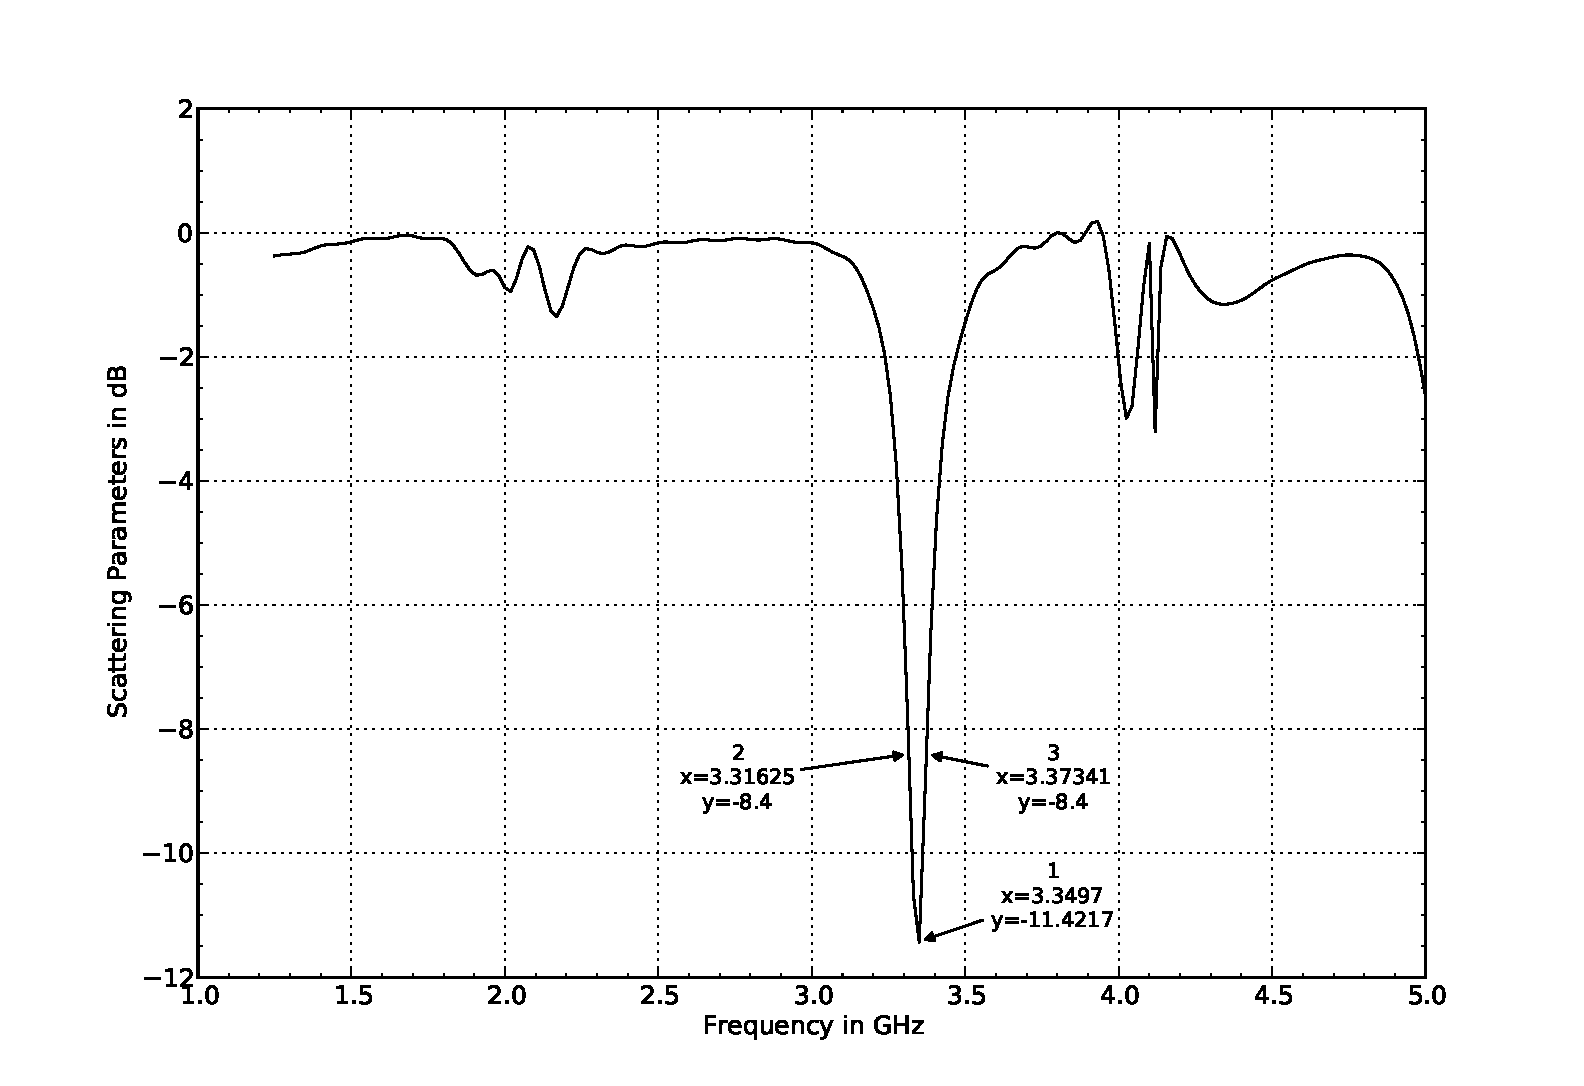
\includegraphics[width=\linewidth]{content/bilder/Evaluation/Loop/ohneABS/S11_Loop_Coil_ohneABS.pdf}
%  \caption{\\$S_{11}$ Diagramm \\einer Loop Antenne \\ im Freiraum}\label{fig:S11_Loop_freiraum_1}
%\endminipage%\hfill
%\minipage{0.4\textwidth}
%  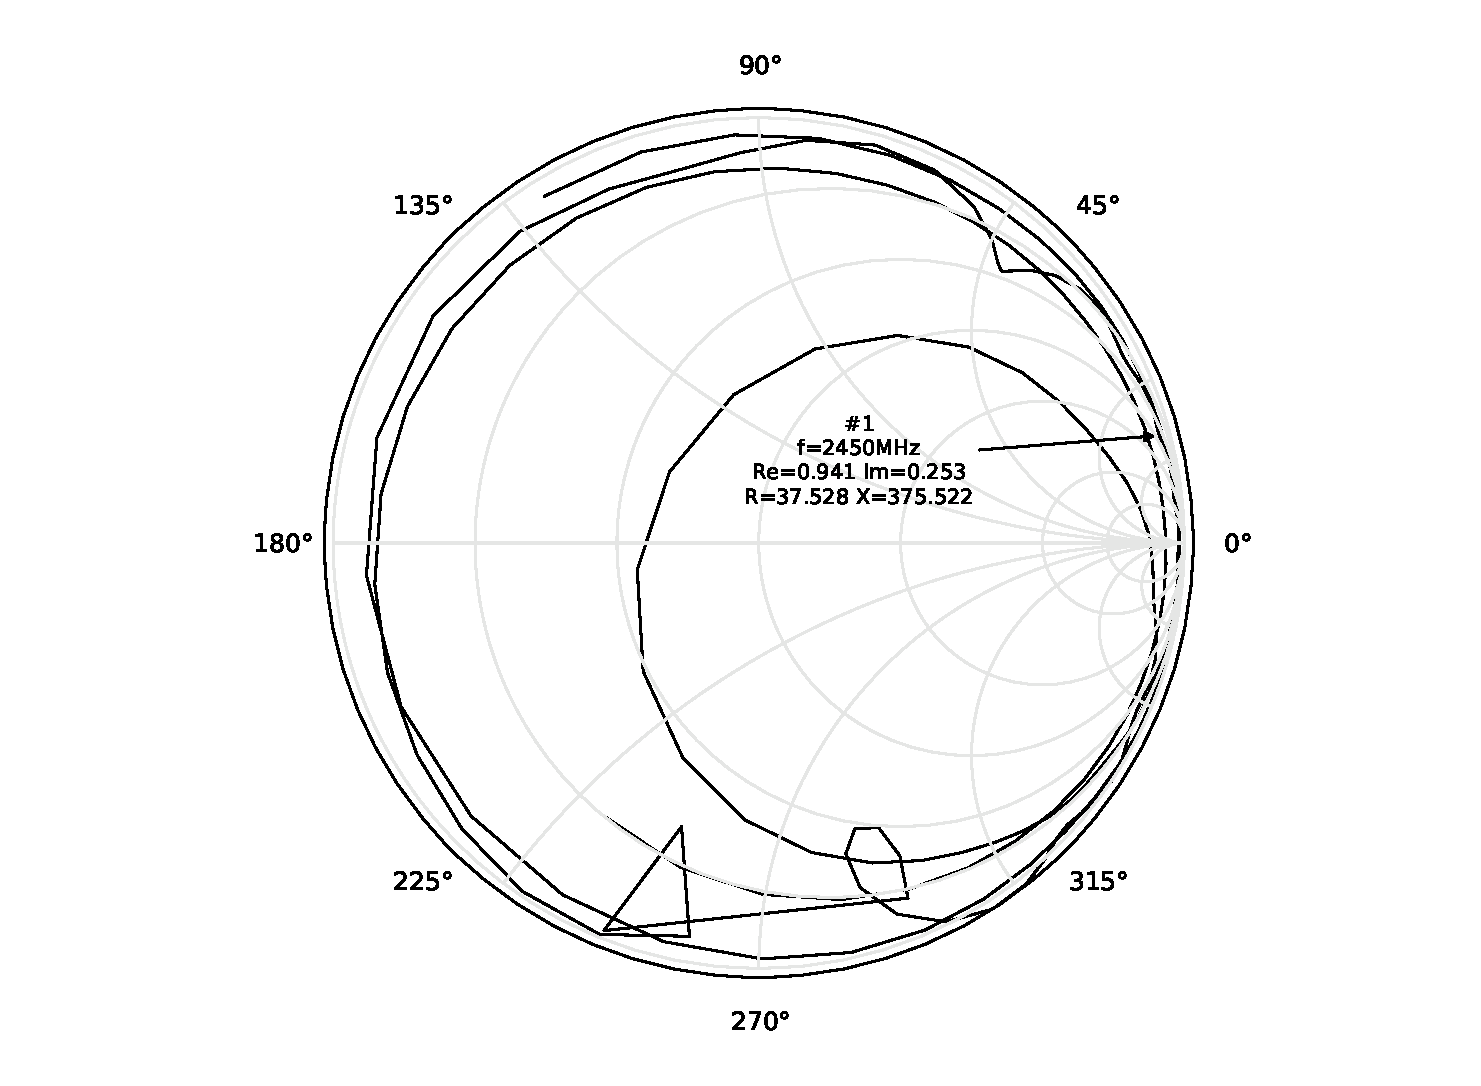
\includegraphics[width=\linewidth]{content/bilder/Evaluation/Loop/ohneABS/Smith_Loop_Coil_ohneABS.pdf}
%  \caption{\\Smith-Diagramm \\einer Loop Antenne \\ im Freiraum}\label{fig:Smith_Loop_freiraum_2}
%\endminipage
%\end{center}
%\end{figure}
%%%%%%%%%%%%%%%%%%%%%%%
Die Abbildung \ref{fig:sim_Loop_3Fach_freiraum_3D} zeigt das 3D Richtdiagramm. Es zeigt sich ein Richtwirkung von 3.4dBi.
%%%%%%%%%%%%%%%%%%%%%
%\begin{figure}[h]
%	\centering
%	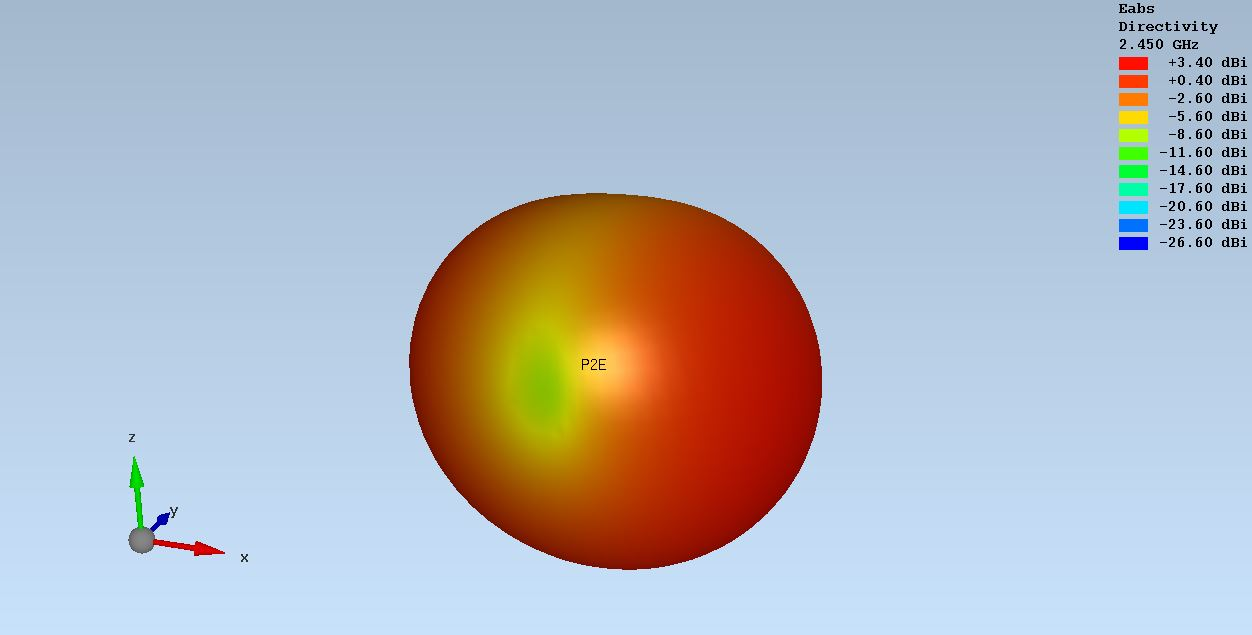
\includegraphics[width=11cm]{content/bilder/Evaluation/Loop/ohneABS/EM_Far_Field_Loop_Coil_ohneABS.JPG}%
%	\caption{Simulierte 3D Abstrahlcharakteristik einer Loop Antenne mit  drei Windungenim Freiraum}
%	\label{fig:sim_Loop_3Fach_freiraum_3D}
%\end{figure}
%%%%%%%%%%%%%%%%%%%%%%%
\newpage
\clearpage
\subsubsection{Simulierte 3D Richtdiagramme einer Loop Antenne mit drei Windungen}
Das Richtdiagramm der dreifachen windungen mit einem angrenzendem Kunststoffstück ist in Abbildung \ref{fig:sim_Loop_3Fach_1ABS_3D} gezeigt. Die maximale Richtcharakteristik weisst einen Wert von 4.55dBi auf.
%%%%%%%%
\begin{figure}[h]
	\begin{center}
		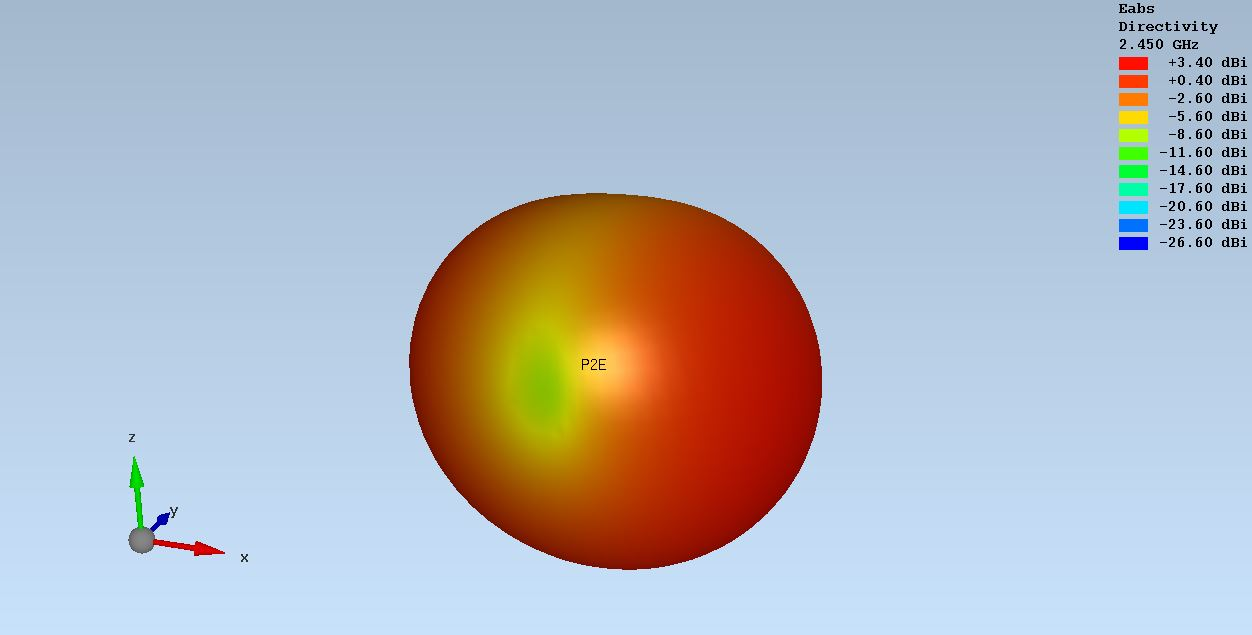
\includegraphics[width=0.9\textwidth]{content/bilder/Evaluation/Loop/ohneABS/EM_Far_Field_Loop_Coil_ohneABS.JPG}
		\captionof{figure}{Simulierte 3D Abstrahlcharakteristik einer Loop Antenne mit  drei Windungen im Freiraum}
		\label{fig:sim_Loop_3Fach_freiraum_3D}
	\end{center}
\end{figure}
\begin{figure}
	\begin{center}
		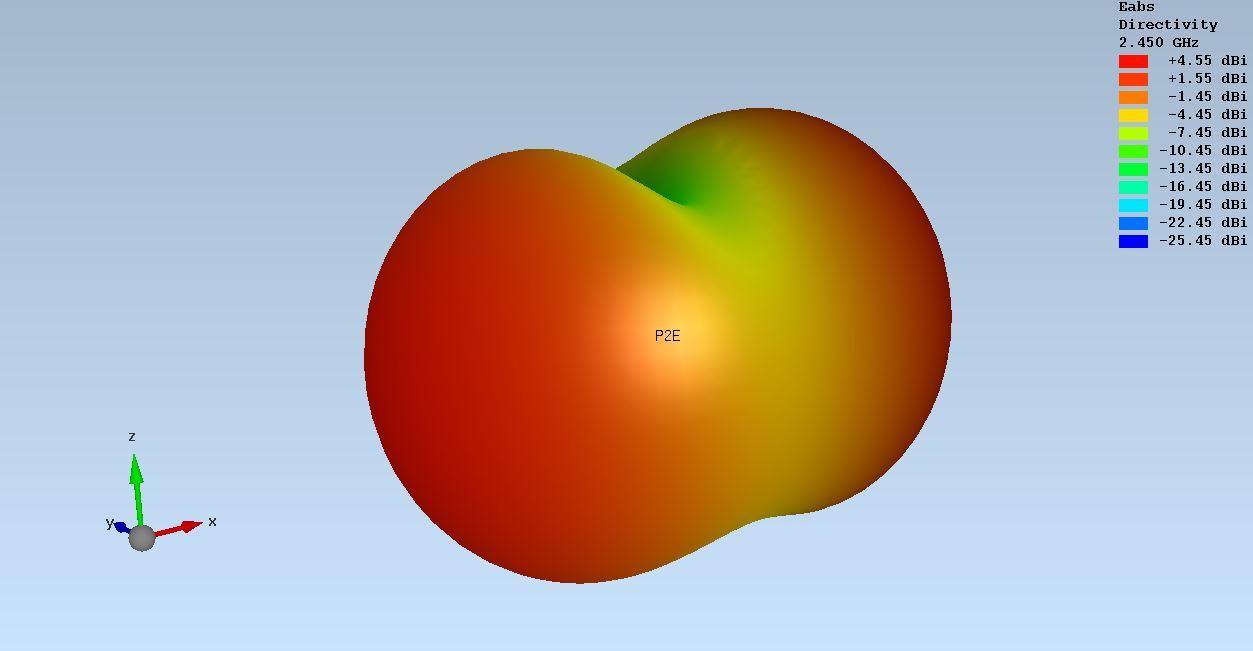
\includegraphics[width=0.9\textwidth]{content/bilder/Evaluation/Loop/Mit1ABS/EM_Far_Filed_Loop_Coil_1ABS.JPG}
		\captionof{figure}{Simulierte 3D Abstrahlcharakteristik einer Loop Antenne mit  drei Windungen  und einem ABS Stück im Nahfeld}
		\label{fig:sim_Loop_3Fach_1ABS_3D}
	\end{center}
\end{figure}
\begin{figure}
	\begin{center}
		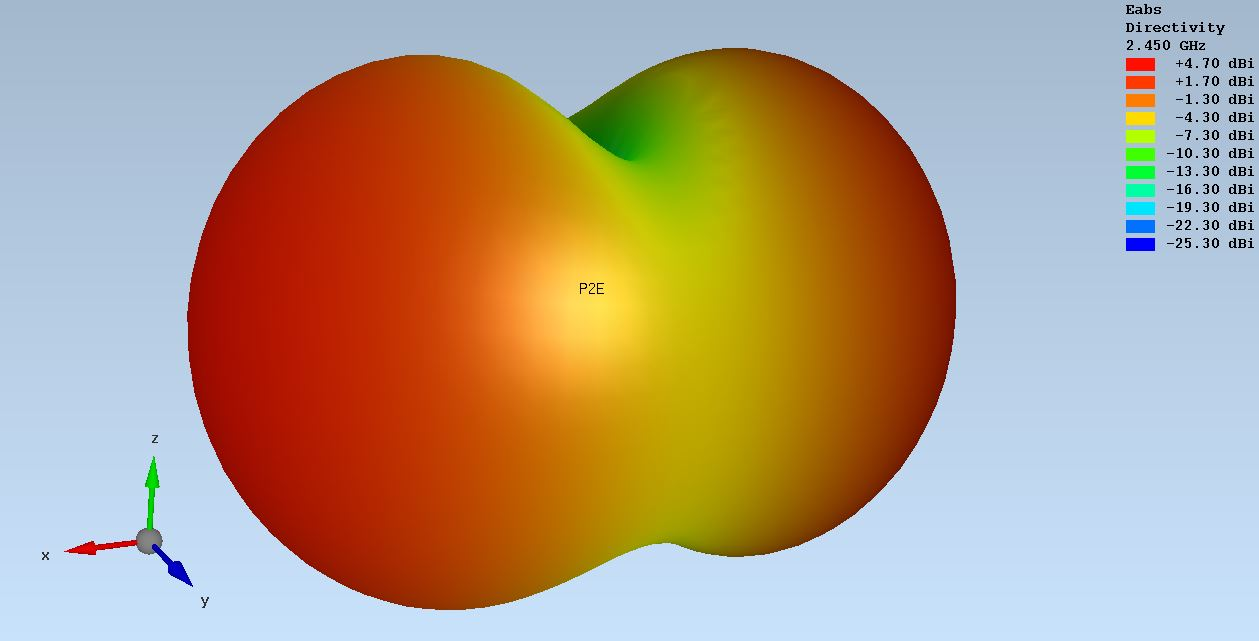
\includegraphics[width=0.9\textwidth]{content/bilder/Evaluation/Loop/Kurz3/EMFraField_Loop_2ABS_kurz3.JPG}
		\captionof{figure}{Simulierte 3D Abstrahlcharakteristik einer Loop Antenne mit  drei Windungen  und zwei ABS Stücken im Nahfeld}
		\label{fig:sim_Loop_3Fach_2ABS_3D}
	\end{center}
\end{figure}
\clearpage
%%%%%%%

%\begin{figure}[!h]
%\begin{center}
%\minipage{0.4\textwidth}
%  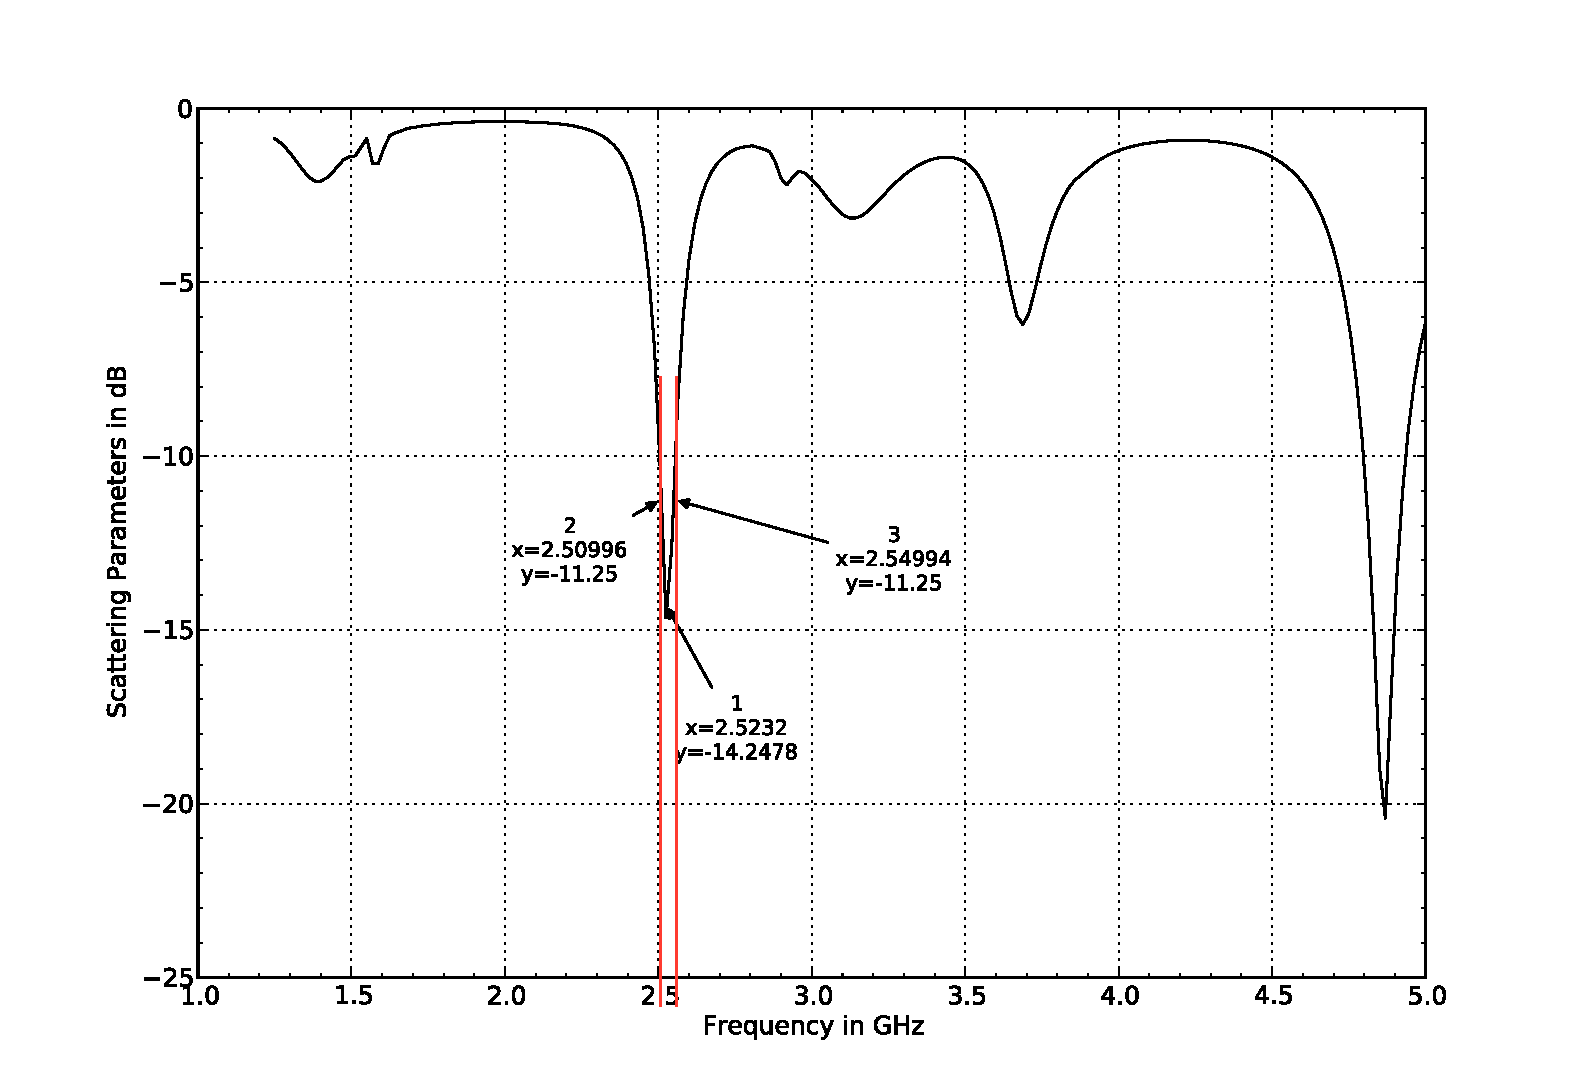
\includegraphics[width=\linewidth]{content/bilder/Evaluation/Loop/mit1ABS/S11_Loop_Coil_1ABS.pdf}
%  \caption{\\$S_{11}$ Diagramm \\einer Loop Antenne \\mit einem ABS Stück im Nahfeld}\label{fig:S11_Loop_1ABS_3}
%\endminipage%\hfill
%\minipage{0.4\textwidth}
%  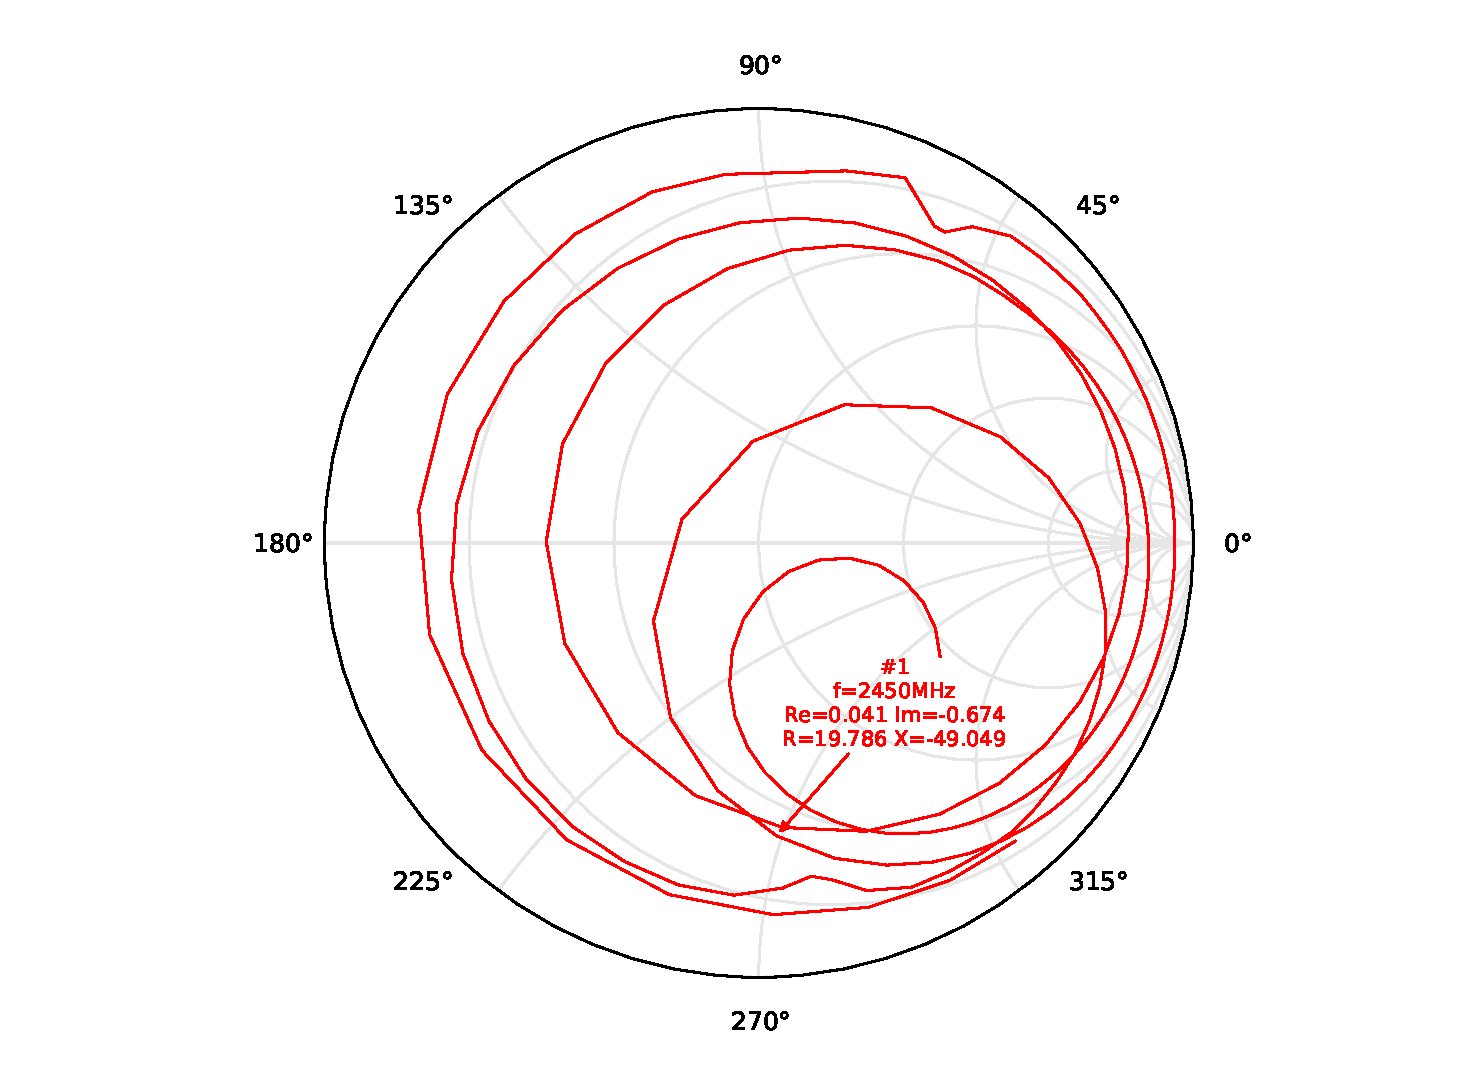
\includegraphics[width=\linewidth]{content/bilder/Evaluation/Loop/mit1ABS/Smith_Loop_Coil_1ABS.pdf}
%  \caption{\\Smith-Diagramm \\einer Loop Antenne \\ mit einem ABS Stück im Nahfeld}\label{fig:Smith_Loop_1ABS_4}
%\endminipage
%\end{center}
%\end{figure}
%%%%%%%%%%%%%%%%%%%%%%%


%%%%%%%%%%%%%%%%%%%%%
%\begin{figure}[h]
%	\centering
%	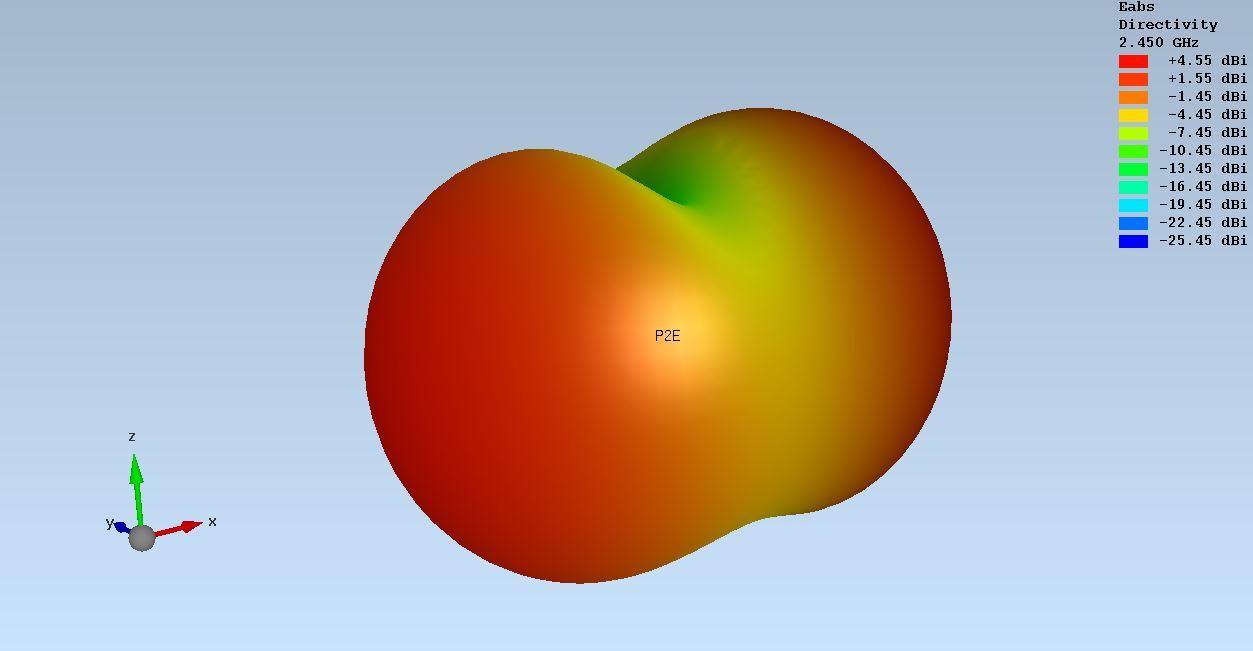
\includegraphics[width=11cm]{content/bilder/Evaluation/Loop/Mit1ABS/EM_Far_Filed_Loop_Coil_1ABS.JPG}%
%	\caption{Simulierte 3D Abstrahlcharakteristik einer Loop Antenne mit  drei Windungenim und einem ABS Stück im Nahfeld}
%	\label{fig:sim_Loop_3Fach_1ABS_3D}
%\end{figure}
%%%%%%%%%%%%%%%%%%%%%%%


%\begin{figure}[!ht]
%\begin{center} 
%\minipage{0.4\textwidth}
%  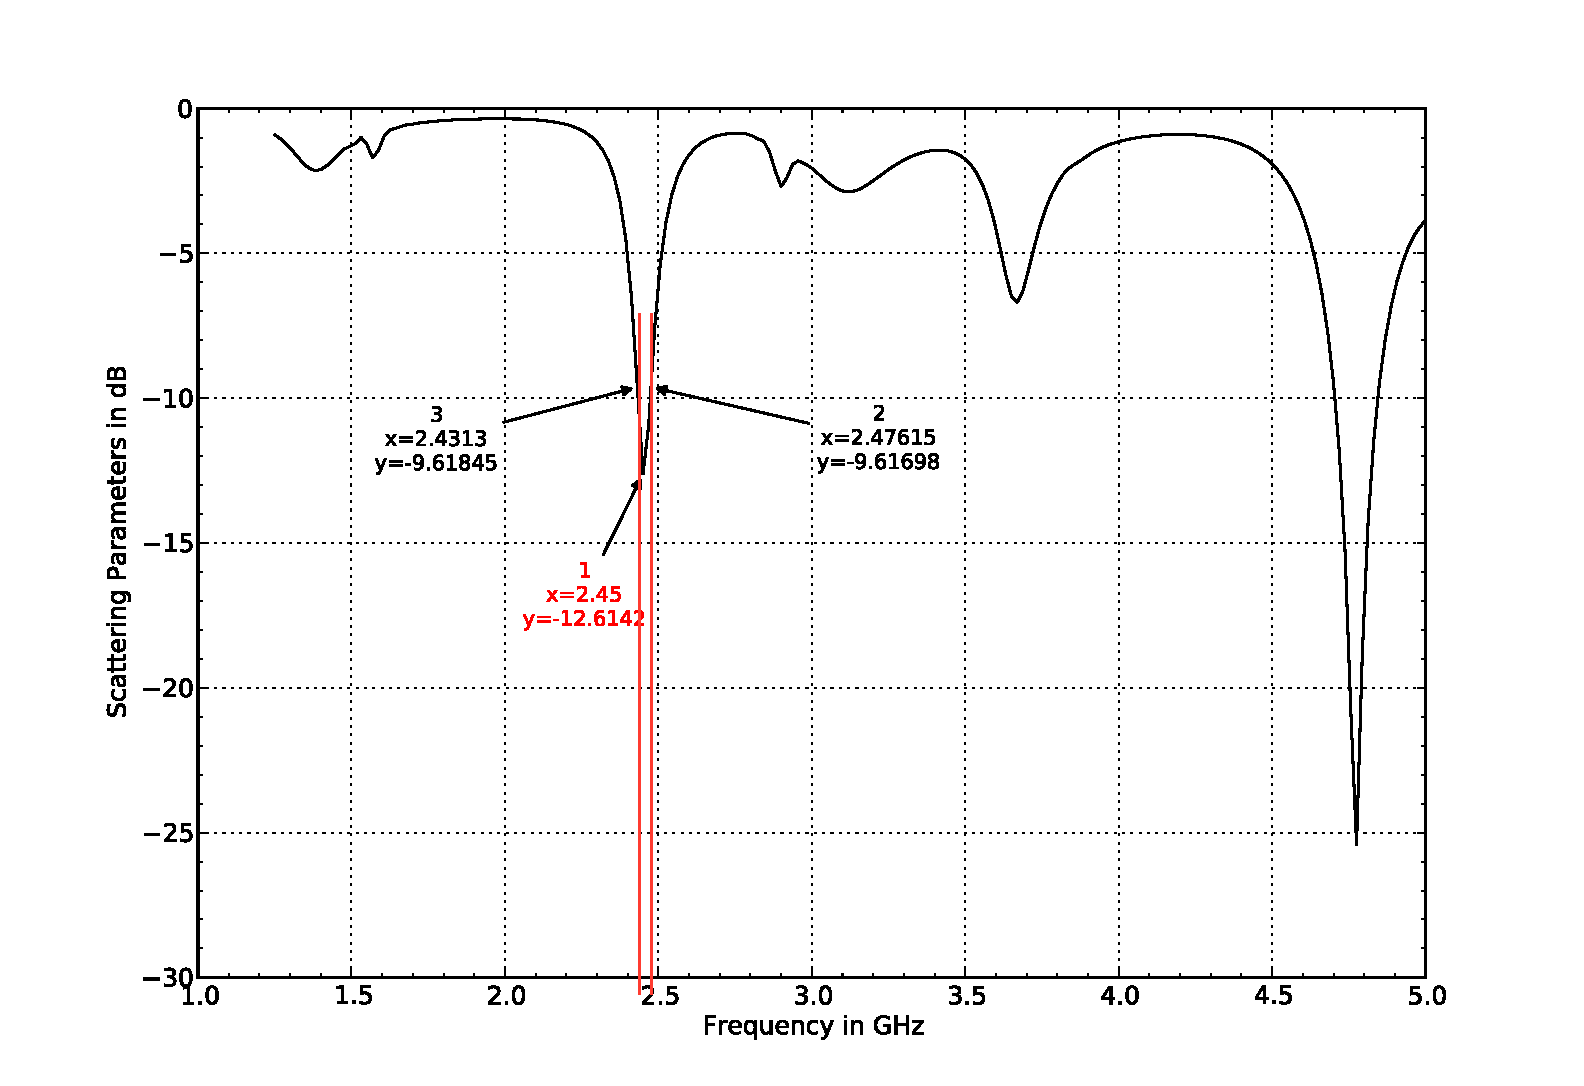
\includegraphics[width=\linewidth]{content/bilder/Evaluation/Loop/Kurz3/S11Loop2ABS.pdf}
%  \caption{\\$S_{11}$ Diagramm \\einer Loop Antenne \\mit zwei ABS Stücken im Nahfeld}\label{fig:S11_Loop_2ABS_5}
%\endminipage%\hfill
%\minipage{0.4\textwidth}
%  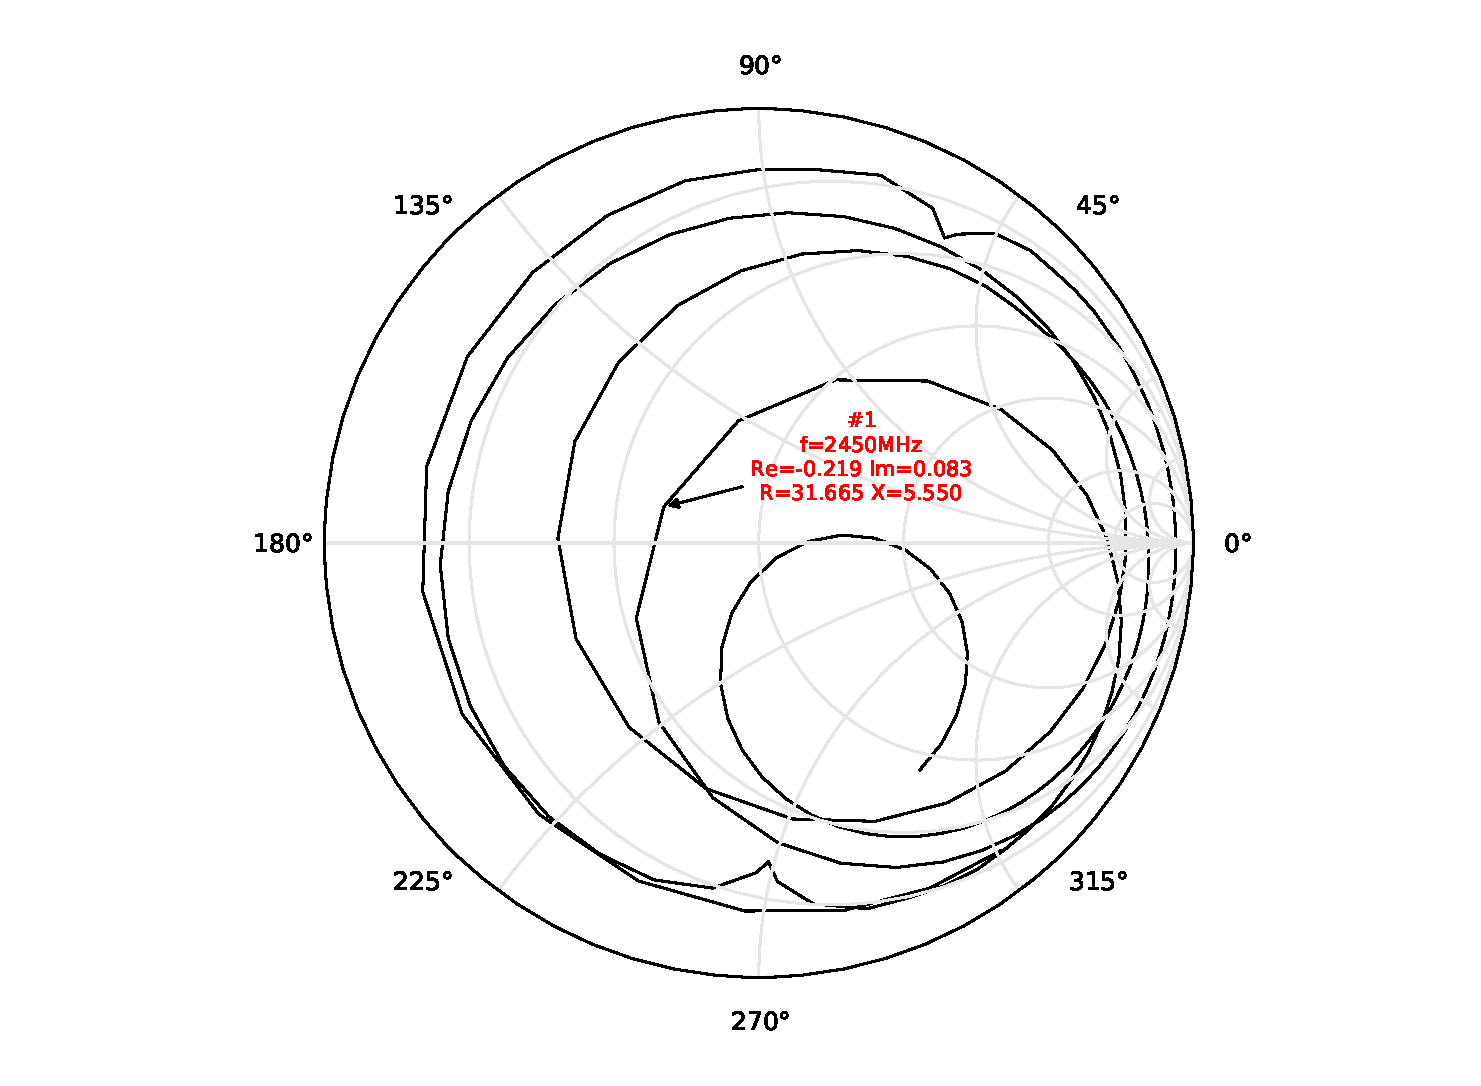
\includegraphics[width=\linewidth]{content/bilder/Evaluation/Loop/Kurz3/SmithLoop2ABS.pdf}
%  \caption{\\Smith Diagramm \\einer Loop Antenne \\mit zwei ABS Stücken im Nahfeld}\label{fig:Smith_Loop_2ABS_6}
%\endminipage
%\end{center}
%\end{figure}
%%%%%%%%%%%%%%%%%%%%%%%


%%%%%%%%%%%%%%%%%%%%%%%
%\begin{figure}[h]
%	\centering
%	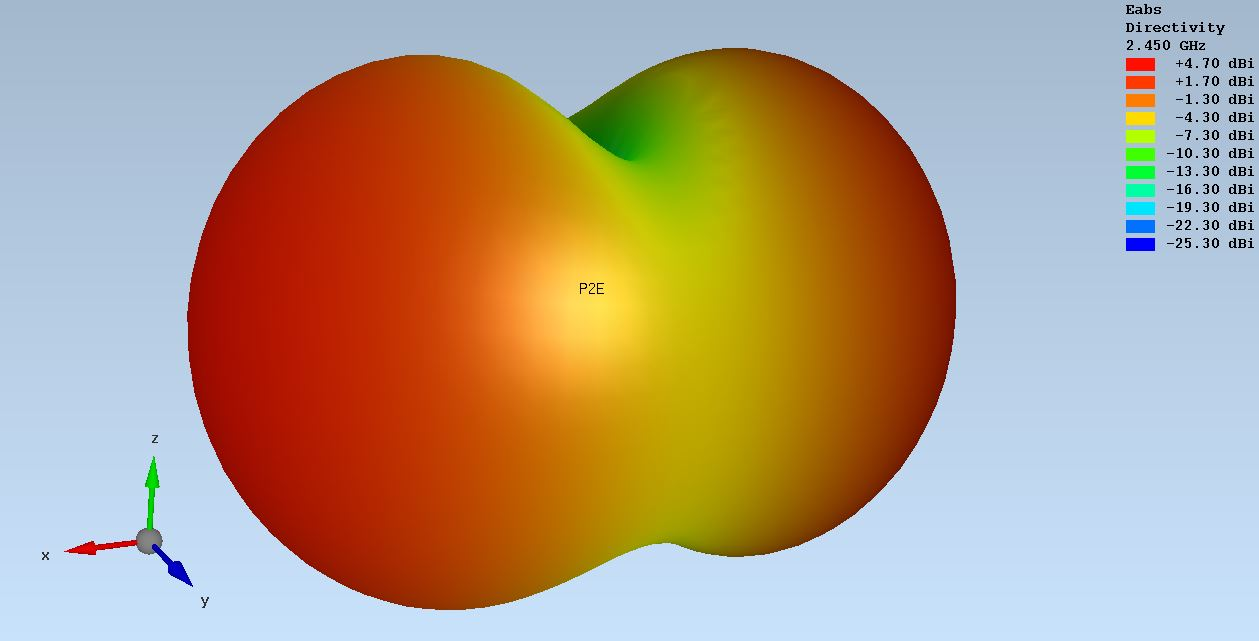
\includegraphics[width=11cm]{content/bilder/Evaluation/Loop/Kurz3/EMFraField_Loop_2ABS_kurz3.JPG}%
%	\caption{Simulierte 3D Abstrahlcharakteristik einer Loop Antenne mit  drei Windungenim und zwei ABS Stücken im Nahfeld}
%	\label{fig:sim_Loop_3Fach_2ABS_3D}
%\end{figure}
%%%%%%%%%%%%%%%%%%%%%%%
\newpage
\subsection{Vergleich aus den Simulationen der Loop Antennen}
Die folgende Tabelle \ref{tab:Evaluation_Vergeich_Dipolantennen} zeigt die wesentlichen Parameter aus den drei Simulationen der $\lambda/2$ Dipolantenne, der $\lambda/2$ Loop Antenne und der Loop Antenne mit drei Windungen. Für jede der Antennen wurden die Werte für die drei Fälle aufgenommen.\\
Fall 1 die Antenne befindet sich im Freiraum.\\
Fall 2 an die Antenne ist ein Kunststoffstück angebracht.\\
Fall 3 die Antenne wird von beiden Seiten von Kunststoffstücken umschlossen.\\
Die Bandbreite beschreibt die -10dB Bandbreite in MHz. Die relative Bandbreite ist ohne Einheit und die Angabe erfolgt in $\%$. Die relative Bandbreite wird durch die Division der -10dB Bandbreite und der Resonanzfrequenz gebildet. Als Resonanzfrequenz wird bei jeder Simulation die Frequenz mit der grössten |$S_{11}$| Dämpfung bestimmt.\\

%Die Tabelle \ref{tab:Evaluation_Vergeich_Dipolantennen} beinhaltet einige Vergleichswerte der $\lambda/2$ Dipolantenne.
%%%%%%%%%%%%%%%%%%%%%%%%%%%%%%%%
%\begin{table}[!h]
%  \centering
%  \begin{tabular}{p{4cm} p{2cm} l  c c c c r} 
%  \toprule 
%  Antenne und Umfeld             & max $S_{11}$[dB]		& $Z_{ant}$[$\Omega$] 	& $\eta$ [$\%$] & Bandbreite & relative Bandbreite[$\%$]\\ 
%  \midrule
%$\lambda/2$ Dipol im Freiraum    			&	-16.16 @ 2.42		&  	68.6-j4			&   	97	&	300[MHz] & 12\\         		
%$\lambda/2$ Dipol mit einem \\ABS Stück 	&   -20.79 @ 2.02  		&	141.5+j39.6		&	71	&	320[MHz]	 & 15\\
%$\lambda/2$ Dipol mit zwei \\ABS Stücken 	&   -28.2 @ 1.81    	&	206.2-j28		&	59	&	320[MHz]	 & 17\\
% \bottomrule
%  \end{tabular}
%  \caption{Simulation einer $\lambda/2$ Dipolantennen im Freiraum und im ABS Stücken}
%  \label{tab:Evaluation_Vergeich_Dipolantennen}
%\end{table}
%%%%%%%%%%%%%%%%%%%%%%%%%%%%%%%%%%%

Die Tabelle \ref{tab:Evaluation_Vergeich_Loop_Antennen_Lmabda05} beinhaltet einige Vergleichswerte der $\lambda/2$ Loop Antenne.
%%%%%%%%%%%%%%%%%%%%%%%%%%%%%%%
\begin{table}[!h]
  \centering
  \begin{tabular}{p{4cm} p{2cm} l  c c c c r} 
  \toprule 
  Antenne und Umfeld             	& max $S_{11}$[dB]		& $Z_{ant}$[$\Omega$] 	& $\eta$ [$\%$] & Bandbreite & relative Bandbreite\\ 
  \midrule
 $\lambda/2$ Loop im Freiraum    		&	-26.2 @ 5.84	&  	2721+j6225			&   1	&	400 & 6.8\\          					   		
$\lambda/2$ Loop mit \\einem ABS Stück &    -15.41 @ 4.41 	&	27.7-j433		&	2.7	&	350 & 7.9 \\
$\lambda/2$ Loop mit zwei \\ABS Stücken &    -13.2 @ 4.30    &	24.5-j379		&	3.1	&	270 & 6.2\\
 \bottomrule
  \end{tabular}
  \caption{Simulation einer $\lambda/2$ Loop Antenne }
  \label{tab:Evaluation_Vergeich_Loop_Antennen_Lmabda05}
\end{table}
%%%%%%%%%%%%%%%%%%%%%%%%%%%%%%%%%%%

Die Tabelle \ref{tab:Evaluation_Vergeich_Loop_Antennen_Coil} beinhaltet die Vergleichswerte der Loop Antenne mit drei Windungen.
%%%%%%%%%%%%%%%%%%%%%%%%%%%%%%%
\begin{table}[!h]
  \centering
  \begin{tabular}{p{4cm} p{2cm} l  c c c c r} 
  \toprule 
  Antenne und Umfeld             & max $S_{11}$[dB]		& $Z_{ant}$[$\Omega$] 	& $\eta$ [$\%$] & Bandbreite & relative Bandbreite\\ 
  \midrule
Loop mit drei Windungen  im Freiraum    		&	-11.4 @ 3.35		&  	37.5+j375			&   	2.2	& 60		& 1.8\\          					   		
Loop mit drei Windungen mit einem ABS Stück 	&    -14.2 @ 2.52  		&	19.8-j49			&	29.5	& 60	 	& 2.3\\
Loop mit drei Windungen mit zwei ABS Stücken &    -12.6 @ 2.45    	&	31.6+j5.5		&	45	& 60 	& 2.4\\
 \bottomrule
  \end{tabular}
  \caption{Simulation einer Loop Antenne mit drei Windungen }
  \label{tab:Evaluation_Vergeich_Loop_Antennen_Coil}
\end{table}
%%%%%%%%%%%%%%%%%%%%%%%%%%%%%%%%%%%
\todo{EinFazit aus den Tabellenwerten ziehen }
\subsection{Interpretation der simulierten Antennen}

Die Nutzwertanalyse zeigt die Vor- und Nachteile der verschiedenen Simulationen auf.
sjadfp

sadjnfp

asüoifj

aspijfdnp


waüeoifhj
sadjnfp

asüoifj

aspijfdnp


waüeoifhj

\newpage
\subsubsection{Nutzwertanalyse der Antenneneigenschaften }
\todo{Text beschreiben}
\begin{table}[!ht]
  \centering
  \begin{tabular}{l r l l l l l l l l} \toprule 
  && \multicolumn{2}{c}{Dipol $\lambda/2$}   && \multicolumn{2}{c}{Loop $\lambda/2$}   && \multicolumn{2}{c}{Loop} \\ \cmidrule{3-4} \cmidrule{6-7} \cmidrule{9-10}
  	Kriterium               	& $g$ \%  		& $N$ & $N\cdot g$     	&& $N$ & $N\cdot g$             		&& $N$ 	& $N\cdot g$ \\ \midrule
  	Antennengüte Q          	&  15          	& 2   & 0.5             	&& 5   & 1.25                        && 5   	& 1.25 \\
  	Impedanz               	&  25           	& 3   & 0.45            	&& 4   & 0.6                         && 5   	& 0.75 \\
	Bandbreite 				&	15			& 4   	& 0.8           	&& 5   & 1 							&&		&	\\
	Relative Bandbreite 		&	10			& 4   	& 0.8           	&& 5   & 1 							&&		&	\\
  	Richtcharakteristik     &  15            & 1   & 0.2            	&& 6   & 1.2                         && 6   	& 1.2 \\
  	Produktionsaufwand    	&   5           & 6   & 0.3             	&& 4   & 0.2                         && 6   	& 0.3 \\
  	Kosten                  &  5           	& 4   & 0.4             	&& 6   & 1.2                         && 6   	& 1 \\
  \hline
  Gesamt                    & 100          	&     & 2.2             	&&     & 5.55                        &&     	& 5.75 \\ \bottomrule
  \end{tabular}
  \caption{Nutzwertanalyse }
  \label{nutzwertEvaluation}
\end{table}


\subsubsection{Antennenkriterien}
\textbf{Antennengüte Q}\\
Bei Antennen wird der Gütefaktor auch Q Wert genannt. Dieser wird aus dem Verhältnis der Mittenfrequenz $F_{c}$ zur Antennenbandbreite B berechnet, wobei die Mittenfrequenz aus dem Mittelwert der oberen und unteren Grenzfrequenz errechnet werden kann. $Q = f_c/(f_0-f_u)$, mit $f_c$ als Mittenfrequenz, $f_u$ als untere Grenzfrequenz und $f_o$ als obere Grenzfrequenz. Je grösser der Gütefaktor, desto schmalbandiger und je niedriger der Gütefaktor,  desto breitbandiger sind Antennen \cite{Guetefaktor_Q}.\\
\textbf{Bandbreite B}\\
In der Nachrichten-, Audio- und Hochfrequenztechnik wird die Bandbreite für einen Frequenzbereich angegeben. Die Bandbreite entspricht dem Frequenzbereich, in dem elektrische Signale mit einem Amplitudenabfall  bis zu einer definierten Grenze. Es handelt sich um eine Frequenzdifferenz zwischen der oberen $f_o$ und der unteren Frequenz $f_u$. Oft ist die Amplitudendgrenze bei -3dB angesetzt. Bei -3dB ist die Signalstärke auf 0.707 des Maxialwerts abgesunken. Das bedeutet, das Signal hat bei -3dB um die Hälfte der maximalen Leistung abgenommen\cite{Bandbreite_B}.
In den Tabellen \ref{tab:Evaluation_Vergeich_Dipolantennen} ,\ref{tab:Evaluation_Vergeich_Loop_Antennen_Lmabda05}, \ref{tab:Evaluation_Vergeich_Loop_Antennen_Coil} und \ref{nutzwertEvaluation} bezieht man sich auf die -10dB Bandbreite.\\
\textbf{Mittenfrequenz $f_{c}$}\\
Die Mittenfrequenz $f_c$ ist definiert über die obere und untere Grenzfrequenz. Sie wird gebildet als $f_c=f_u+(f_o-f_u)/2$. Die Mittenfrequenz muss nicht der Resonanzfrequenz $f_{res}$ entsprechen.\\
%%%%%%
\textbf{Relative  Bandbreite d}\\
Die relative Bandbreite ist der Kehrwert der Antennegüte Q.
Sie wird gebildet, in dem die Bandbreite B durch die Resonanzfrequenz $f_{res}$ geteilt wird. $d=\dfrac{Bandbreite}{f_{Resonanz}}$\\
%%%%%%
\textbf{Richtcharakteristik D}\\
Die Richtcharakteristik ist das Verhältnis der maximalen Leistungsdichte der Antenne gegenüber einem isotropen Strahler in dBi.\\
\textbf{Abstrahleffizienz $\eta$}\\
Man unterscheidet zwischen $\eta_{rad}$ und $\eta_{Total}$. Die Abstrahleffizienz des Strahlungswiderstands ist definiert als $\eta_{rad}=\dfrac{R_{rad}}{R_{rad}+R_v}$. Die totale Abstrahleffizienz ist immer an die Impedanz und Leistung der Zuleitung gebunden. Sie berechnet sich als $\eta_{Total}=\dfrac{P_{rad}}{P_{Leitung}+P_{rad}}$. In diesem Kapitel ist immer die totale Abstrahleffizienz erwähnt.\\
\textbf{Antennenimpedanz $Z_{ant}$}\\
Die Antennenimpedanz ist eine komplexe Grösse. Sie fasst alle Real- und Imginärteile der Antenne in einem Wert zusammen.\\
\textbf{Produktionsaufwand}\\
Eine Schätzung, wie aufwenig ein Produkt herzustellen ist. Die Anzahl der Arbeitsschritte oder die Menge und die Verfühgbarkeit der Materialen werden berücksichtigt.\\
\textbf{Kosten}\\
Eine Abschätzung wie Kostenintensiv ein Produkt ist.
\newpage 
\thispagestyle{empty}

